\part{SYSTEMS AND SYSTEMS THINKING}\label{part:1}

Systems engineering and analysis is promulgated most effectively when supported by insight about important system domains having high-level association.  That is the purpose of four chapters comprising \Cref{part:1} of this textbook.  The relevant domains are the world in which we live, systems thinking and knowledge, organization and enterprise systems, and economics and enterprise economy. Together these provide a prerequisite foundation for the synthesis, analysis, and evaluation of engineered systems; engineered systems being the central focus of this book.
	
The first chapter introduces the world in which we live as the overarching system of primary interest. When partitioned into interconnected natural, human-made, and human-modified sectors, it is found that human activities may be traced and evaluated at high levels with purpose and confidence.
	
\Cref{chap:02} has a science and systems science orientation.  It covers general system definitions and ends with contemporary definitions of systems engineering.  Between these important definitional categories is a conceptual discussion of system elements, a high-level classification of systems, a summary of science and systems science, and a view of technology as the progenitor for engineered systems.
	
Cooperation through organization is essential for human progress. It addressed in \Cref{chap:03} as humankind’s most important innovation. The role of purposeful human action, known as praxeology, is emphasized as being most relevant to systems thinking and enterprise systems.
	
Praxeology also underpins \Cref{chap:04}, focused on economics and enterprise economy.  Here the human action form of economic thinking is featured as the basis for economic progress. Taken together, these last two chapters address organization as humankind’s most important innovation within the pervasive economic setting for enterprises and the economy.

\Cref{part:1} of this textbook has the potential to stand alone as a learning module.  It provides a high-level introduction to systems, science, engineering, and systems engineering that will be suitable for discussion with engineering and technical people.  Subsequent chapters should be considered only after obtaining an understanding of the fundamentals in Part I, but study beyond these fundamentals is optional for those who need only an overview of systems engineering and its foundation in systems analysis.

%%----------------------------------------------------------------------------------------
%	PART CONTENT
%%----------------------------------------------------------------------------------------

\chapterimage{purpleLeaf.jpg} % Chapter heading image
\chapter{THE WORLD IN WHICH WE LIVE} \label{chap:01}

The world in which we live is known more to us than is the universe or, perhaps, universes in which it exists.  This world is known to be part of a solar system which is known to be part of a universe made up of similar solar systems and galaxies.  We know more about the world in which we live than we do about the universe in which it resides.  In fact, the purposes of this textbook are realized independent of knowing any more of a universal nature extant above and beyond our world.

The primary purpose of this textbook may be addressed directly by recognizing the ultimate system of interest in STEA to be \textit{the world in which we live}.  We observe the \textit{natural}, the \textit{human-made}, and the \textit{human-modified} worlds to be interconnected sectors as illustrated in \Cref{fig:humanModifiedVennDiagram}.  Of these, it is the human-modified world that should be adopted as the highest-level system of our concern, because that is where we actually live.

\begin{figure}[h]
\centering
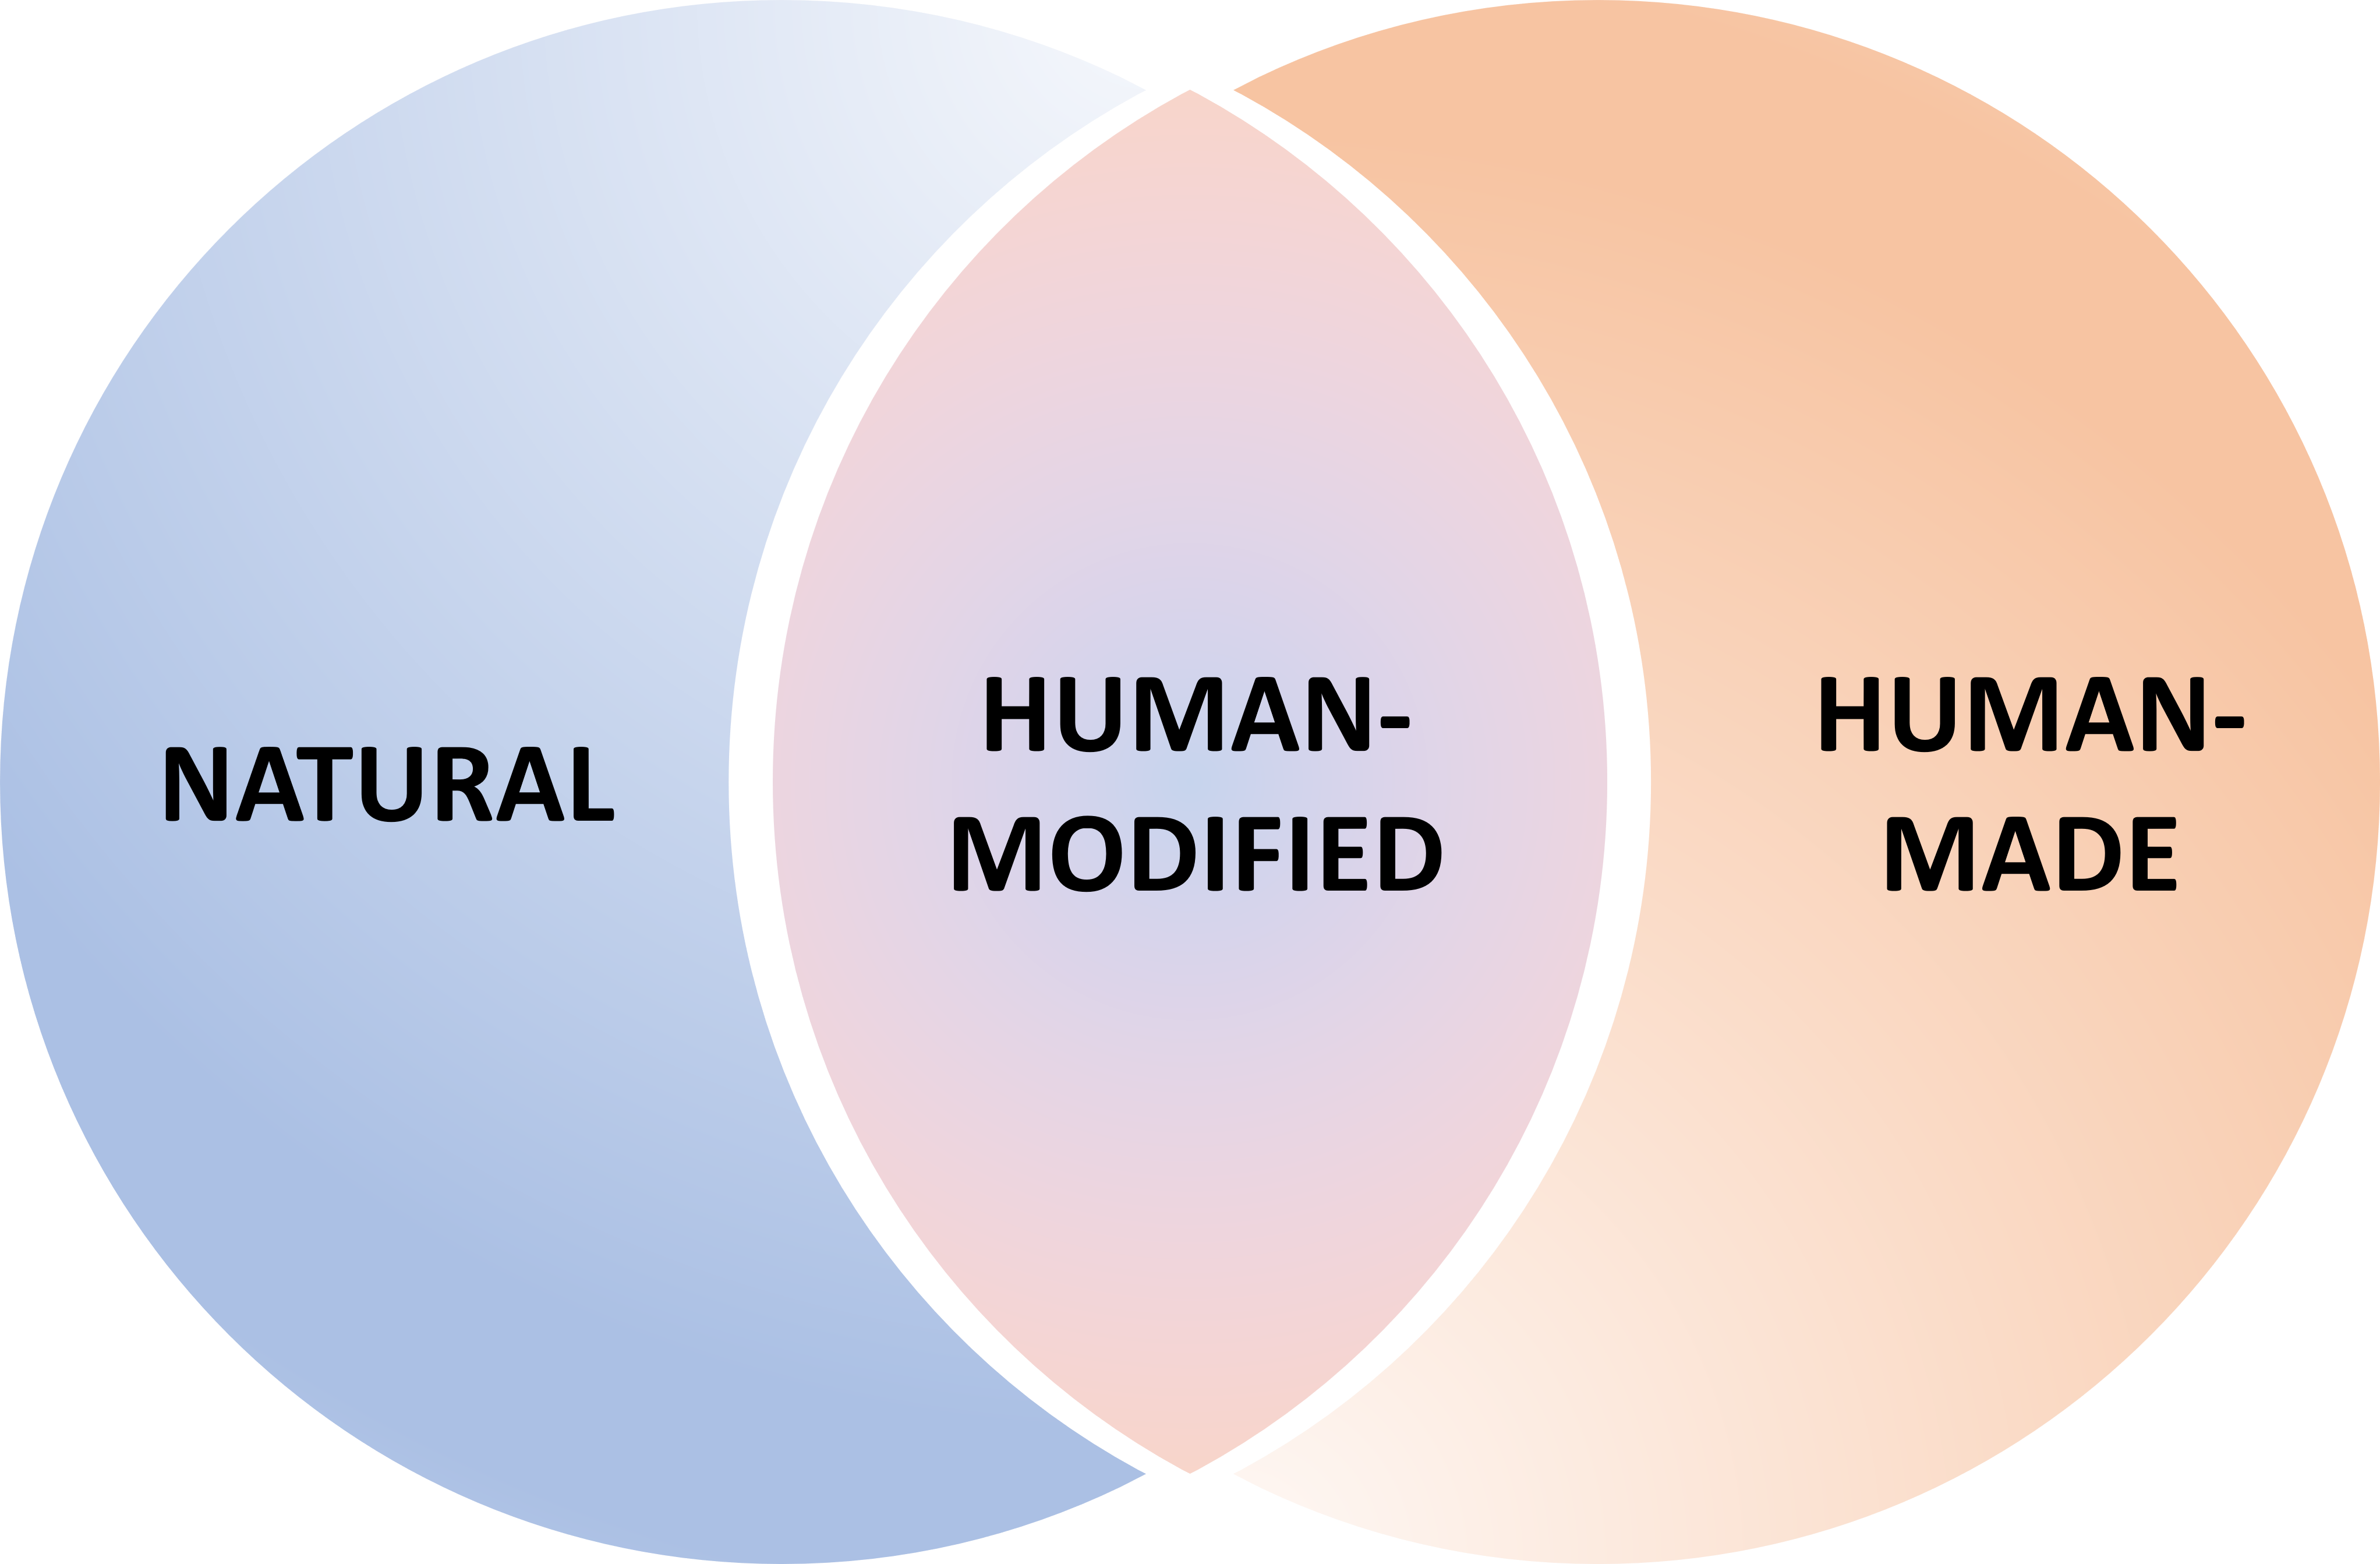
\includegraphics[width=0.9\textwidth]{humanModifiedVennDiagram.png}
\caption{Our world viewed as interconnected sectors.}
\label{fig:humanModifiedVennDiagram}
\end{figure}
    
The natural world came into being by natural processes.  The human-made world is made up of systems and products that resulted from the intervention of humans through components, attributes, and relationships.  The \textit{human-modified world} is the natural world into which the human-made has been introduced as systems, subsystems, entities, and artifacts; a world becoming increasingly complex.  This book strives to justify the human-modified world as the ultimate system level at which the viability of all that is human made should be judged.

%%----------------------------------------------------------------------------------------
%	CHAPTER CONTENT
%%----------------------------------------------------------------------------------------

\section{Sectors Comprising Our World}\index{Sectors Comprising Our World}\label{sec:sectorsComprisingWorld}

The world in which we live may be divided into the natural world and the human-made world.  Included in the former are all elements of the world that came into being by natural processes. The human-made world is made up of all human-originated systems, their product subsystems (including structures and services), and their other subsystems (such as those for production and support).  But it is the advent of the human-made that has resulted in a human-modified world as the actual world in which we live.

Systems are as pervasive as the universe in which they exist.  They are as grand as the universe itself or as infinitesimal as the atom.  This is, however, beyond the scope of STEA and requires reduction into sectors comprising our world.  Systems appeared first in natural forms, but with the advent of human beings a variety of human-made systems have come into existence.

The origin of systems gives the most important classification opportunity.  \textit{Natural systems} are those that came into being by natural processes.  \textit{Human-made systems} are those in which human beings have intervened through component, attributes, and relationships.  The \textit{human-modified system} is a natural system into which a human-made system has been integrated.

\subsection{The Natural World}\index{The Natural World}\label{sec:NaturalWorld}

The natural world is made up of all systems, including humans, that came into being by natural processes without human involvement. \textit{Natural systems} are those that came into being by natural processes. \textit{Human-made systems} are those in which human beings have intervened through components, attributes, and relationships. 

All human-made systems, when brought into being, are embedded into the natural world. Important interfaces often exist between human-made systems and natural systems. Each affects the other in some way. The effect of human-made systems on the natural world has only recently become a keen subject for study by concerned people, especially in those instances where the effect is undesirable. In some cases, this study is facilitated by analyzing the natural system as a human-modified system.

When designing a human-made system, undesirable effects can be minimized—and the natural system can sometimes be improved—by engineering the larger human-modified system instead of engineering only the human-made system. If analysis, evaluation, and validation of the human-modified system are appropriate, then the boundary of the environmental system—drawn to include the human-made system—should be considered the boundary of the human-modified system.

Natural systems exhibit a high degree of order and equilibrium. This is evidenced in the seasons, the food chain, the water cycle, and so on. Organisms and plant life adapt themselves to maintain equilibrium with the environment. Every event in nature is accompanied by an appropriate adaptation, one of the most important being that material flows are cyclic. In the natural environment there are no dead ends, no wastes, only continual re-circulation and regeneration.

Only recently have significant human-made systems appeared. These systems make up the human-made world, their chief engineer being human. The rapid evolution of human beings is not adequately understood, but their arrival has significantly affected the natural world, often in undesirable ways. Primitive beings had little impact on the natural world, for they had not yet developed potent and pervasive technologies.

An example of the impact of human-made systems on natural systems is the set of problems that arose from building the Aswan Dam on the Nile River. Construction of this massive dam ensures that the Nile will never flood again, solving an age-old problem. However, several new problems arose. The food chain was broken in the eastern Mediterranean, thereby reducing the fishing industry. Rapid erosion of the Nile Delta took place, introducing soil salinity into Upper Egypt. No longer limited by periodic dryness, the population of bilharzia (a waterborne snail parasite) has produced an epidemic of disease along the Nile. These side effects were not adequately anticipated by those responsible for the project. A system view encompassing both natural and human-made elements, as a human-modified system, might have led to a better solution to the problem of flooding. (Look for a better / more general example).


An example of the impact of human-made systems on natural systems is the set of problems that arose from building the Aswan Dam on the Nile River\footnote{\href{http://www.edc.uri.edu/temp/ci/ciip/FallClass/Docs_2006/UrbanWaterfronts/Abu-Zeid\%20and\%20El-Shibini.pdf}{Aswan Dam on the Nile}}. Construction of this massive dam ensures that the Nile will never flood again, solving an age-old problem. However, several new problems arose. The food chain was broken in the eastern Mediterranean, thereby reducing the fishing industry. Rapid erosion of the Nile Delta took place, introducing soil salinity into Upper Egypt. No longer limited by periodic dryness, the population of bilharzia (a waterborne snail parasite) has produced an epidemic of disease along the Nile. These side effects were not adequately anticipated by those responsible for the project. A system view encompassing both natural and human-made elements, as a human-modified system, might have led to a better solution to the problem of flooding.

\subsection{The Human-Made World}\index{The Human-Made World}\label{subsec:humanMadeWorld}

The human-made world is made up of all systems wherein humans have intervened through components, attributes, and relationships.

All human-made systems, when brought into being, are embedded into the natural world. Important interfaces often exist between human-made systems and natural systems. Each affects the other in some way. The effect of human-made systems on the natural world has only recently become a keen subject for study by concerned people, especially in those instances where the effect is undesirable. In some cases, this study is facilitated by analyzing the natural system as a human-modified system.

When designing a human-made system, undesirable effects can be minimized - and the natural system can sometimes be improved - by engineering the larger human-modified system instead of engineering only the human-made system. If analysis, evaluation, and validation of the human-modified system are appropriate, then the boundary of the environmental system - drawn to include the human-made system - should be considered a boundary of the human-modified system.
	
Natural systems exhibit a high degree of order and equilibrium. This is evidenced in the seasons, the food chain, the water cycle, and so on. Organisms and plant life adapt themselves to maintain equilibrium with the environment. Every event in nature is accompanied by and appropriate adaptation, one of the most important being that material flows are cyclic. In the natural environment there are no dead ends, no wastes, only continual recirculation and regeneration.

Only recently have significant human-made systems appeared. These systems make up the human-made world, their chief engineer being human. The rapid evolution of human beings is not adequately understood, but their arrival has significantly affected the natural world, often in undesirable ways. Primitive beings had little impact on the natural world, for they had not yet developed potent and pervasive technologies.

	Interesting. From a biologist’s point of view the following...
    
Anything a beaver, or even army ants, or colonial termites make is natural because it is made by a natural entity. Presumably evolution has very strongly selected for that which is made by them by eliminating many other alternatives as they arose. This ensures that at least for the near term, such innovations are fit within the environment. Until the environment changes which it usually does in the very long term.

But then why make a distinction for humans?  We have evolved also. We are natural entities. Why wouldn’t anything we make be burdened with the term “artificial” than any other thing made by a tool-using social organism?  Persons focusing only on these aspects would see the natural vs artificial controversy as empty and unnecessary.

Now, I did not make up that distinction but do use it often. All human systems including our socio-economic and socio-political institutions I consider immature artefacts. In fact, it was Nobel Laureate Herbert Simon, in whose honor NECSI grants an annual award, and whose famous book was titled, “Sciences of the Artificial” who first popularized use of the term.

Perhaps it is because scientists realize that anything man makes can be engineered so quickly that it is not subject to natural selection and evolution at first and then not even for a very long time afterward if at all. So, products that reflect more greed than adaptation to context, more arrogance than fit within natural parameters, surround our civilization. This might give some meaning to artificial. Further, the distinction might lead to a regime in which prescription and values become an important part of the process, recycling and fit in environment and cost-to-benefit an important part of the process in addition to making a buck. Len.

\subsection{Natural Versus Human-Made World}\index{Natural Versus Human-Made World}\label{subsec:naturalVsHumanWorld}

How do we classify a beaver dam?  Is it artificial or natural?  Clearly it is not designed and made by humans. This should keep the ontology folks busy.
	
To what extent is human activity not considered a part of nature? Or, do we define as synthetic anything done by the hand of man?

The universe is composed of stateful objects that undergo transformations via processes – patterns of object transformations that we as humans conceptualize in order to be able to think about cause-and-effect along the timeline.

We distinguish between natural and man-made systems (and I think they should be called by different names) because value and free will apply only to humans.

The definition of system then depends on whether it is natural or artificial.

An artificial system is an object that fulfills a function – a value-adding process from some beneficiary’s perspective.

A natural system is a collection of natural objects that are structured and behave following laws of nature.

In the discussion of “natural” vs. “man-made”, it is clear that we must decide whether to consider “man” to be a part of “nature” in the context of the discussion.

Men build dams, but we do not consider the Hoover Dam to be natural. Beavers make dams, but we deem them to be natural. Therefore, one might conclude the “we” do not consider man to be “natural” (neither man, nor his actions) in the context of the discussion. This could get downright philosophical and theological, but that is not the point.

So, are “natural” and “man-made” the words we want to use to define the concepts of “everything man DOES NOT DO” from “everything man DOES DO?”  Then, we must determine how to classify that which arises from an interaction between the two.
    
\subsection{The Human-Modified World}\index{The Human-Modified World}\label{subsec:humanModifiedWorld}

The Human-Modified World is composed of natural systems from which resources are extracted and human-made systems are embedded. We don’t live in the natural world. We don’t live in the human-made world. We live in a hybrid world at the intersection of the two already identified as the Human-Modified World. There is nothing that we do as humans that does not have one foot in the natural world and the other in the human-made world.

Since the very beginning of their existence, humans have struggled to cope with the world into which they…appeared. Knowledge, organization, and economics are the primary enablers. Human conceived existence enablers . . . 

A human-modified system is a natural system into which a human-made system has been integrated as a subsystem.

Twentieth Century man, more than his ancestors, must attempt to understand the varied peoples with whom he shares an increasingly small planet. To reach this understanding he needs to know the cultures which molded other peoples’ outlook, the history that carried them to this point.

How to select the civilizations that must be examined in a limited series of books on the history of the world’s cultures?  That is the subject of Jaques Barzun’s introduction to the Time-Life series entitled The Great ages of Man. Mr. Barzun, Dean of Faculties and Provost of Columbia University, is one of the pre-eminent cultural historians of this generation. He describes how the “revolution … in our conception of humanity” wrought by the emergence of “dozens of new peoples, new states, and new pasts” has made essential the realization that “nothing human is alien.”

In explaining the criteria for the selection of historic cultures examined in this series, he also suggests the path that present-day cultures may follow in the future.

THE EDITORS OF TIME-LIFE BOOKS (1965 Time Inc.) This book strives to justify the human-modified world as the ultimate system level at which the viability of all that is human-made should be judged. Systems thinking reveals the shortcomings of this obvious but limiting bifurcation. Consider stepping back from “The inherently presumptuous notion of human-made in favor of a continuum that starts with acceptance of the natural world as the original, or default state. Emanating from the ‘created’ state comes recognition of the advent of increasingly potent modifications by humans. The complex embedded systems that now serve humanity constitute a progressively advancing continuum between the beginning and now.”

As an example, the impact of human-made systems on natural systems is the set of problems that arose from building the Aswan Dam on the Nile River. Construction of this massive dam ensures that the Nile will never flood again, solving an age-old problem. However, several new problems arose. The food chain was broken in the eastern Mediterranean, thereby reducing the fishing industry. Rapid erosion of the Nile Delta took place, introducing soil salinity into Upper Egypt. No longer limited by periodic dryness, the population bilharzia (a waterborne snail parasite) has produced an epidemic of disease along the Nile. These side effects were not adequately anticipated by those responsible for the project. A systems view encompassing both natural and human-made elements, as a human-modified system, might have led to a better solution to the problem of flooding.

When brought into being, all that is human-made are embedded into the natural world. Important interfaces exist between human-made systems and natural systems. Each affects the other in many ways. The effect of human-made systems on the natural world has only recently become a keen subject for consideration by concerned people, especially when the effect is deemed undesirable.

Only recently have significant and complex human-made systems appeared. These systems make up the human-made world, their chief engineer being human. The rapid appearance of human beings is not adequately understood, but human presence has significantly affected the natural world, too often in undesirable ways. Primitive beings had little impact on the natural world, for they had not yet developed pervasive and potent enabling technologies.
\section{General Understanding of Systems}\index{General Understanding of Systems}\label{sec:generalUnderstandingSystems}

A system is a set of interconnected elements which form a whole and show properties which are properties of the whole rather than of the individual elements. This definition is valid for a cell, an organism, a society, or a galaxy. Joanna Macy says that a system is less a thing than a pattern – a pattern of organization. It consists of a dynamic flow of interactions which is non-summative, irreducible, and integrated at a new level of organization permitted by the interdependence of its part. The word “system” derives from the Greek “synhistanai” which means “to place together.”

From a cognitive perspective, systems thinking integrates analysis and synthesis. Natural science has been primarily reductionistic, studying the components of systems and using quantitative empirical verification. Human science, as a response to the use of a positivistic methods for studying human phenomena, has embraced more holistic approaches, studying social phenomena through qualitative means to create meaning. Systems thinking bridges these two approaches by using both analysis and synthesis to create knowledge and understanding and integrating an ethical perspective.

Analysis answers the ‘what’ and ‘how’ questions while synthesis answers the ‘why’ and ‘what for’ questions. By combining analysis and synthesis, systems thinking creates a rich inquiring platform for approaches such a social systems design, developed by Bela H. Banathy, and evolutionary systems design, as Alexander Laszlo and myself have developed to include a deeper understanding of a system in its larger context as well as a vision of the future for co-creating ethical innovations for sustainability. Just like the first image of Earth from outer space had a huge impact on our ability to see the unity of our planet, systems thinking is a way of seeing ourselves as part of larger interconnected systems.

Systems thinking is a gateway to seeing interconnections. Once we see a new reality, we cannot go back and ignore it. More importantly, that “seen” has an emotional connection, beautifully captured in the statement by Rusty Schweickart after his experience of seeing his home planet from space. – Oliver W. Holmes

What are the emotions evoked by perceiving for the first time the unity, interconnectedness, and relatedness of a system?  What are the feelings evoked by perceiving and experiencing disconnection and isolation?  Humberto Maturana says that “emotions are fundamental to what happens in all our doings” and yet, bringing up emotions in a scientific or business conversation is in many cases considered irrelevant, inappropriate or simply uncomfortable. Following Maturana’s views, I would say that the simplified answer to my two questions on the emotions evoked by unity and disconnection are love and fear, correspondingly. Love is the only emotion that expands intelligence, creativity and vision; it is the emotion that enables autonomy and responsibility. Maturana defines love as “relational behaviors through which another (a person, being, or thing) arises as a legitimate other in coexistence with oneself.”  Only in a context of safety, respect and freedom to be and create (that is, a context of love) can people be relaxed and find the conditions conductive to engage in higher intelligent behaviors that uses their brain neocortex. Learning, collaboration and creativity happen when we are able to function from a consciousness capable of including a world centric awareness of “all of us”, as Ken Wilber puts it. On the contrary, in a situation of stress, insecurity, or any other manifestation of ear, we are conditions to react more instinctually and to operate from our reptilian brain to fulfil more rudimentary needs linked to survival.

The first image of our whole Earth from space created a sense of awe and beauty. From space, we can see (and feel) its wholeness: there are no political lines dividing our national territories, there is only one whole system. However, from our terrestrial and regionally bounded experiences, we can feel that the neighbor tribe is sufficiently different and threatening to be considered an enemy.

Systems being involves embodying a new consciousness, an expanded sense of self, a recognition that we cannot survive alone, that a future that works for humanity needs also to work for other species and the planet. It involves empathy and love for the greater human family and for all our relationships – plants and animals, earth and sky, ancestors and descendants, and the many peoples and beings that inhabit our Earth. This is the wisdom of many indigenous cultures around the world, this is part of the heritage that we have forgotten, and we are in the process of recovering.

Systems being and systems living brings it all together: linking head, heart, and hands. The expression of systems being is an integration of our full human capacities. It involves rationality with reverence to the mystery of life, listening beyond words, sensing with our whole being, and expressing our authentic self in every moment of our life. The journey from systems thinking to systems being is a transformative learning process of expansion of consciousness – from awareness to embodiment.

Kathia Laszlo, Ph.D., directs Saybrook University’s program in Leadership of Sustainable Systems. This post is an excerpt from the plenary presentation “Beyond Systems Thinking: The role of beauty and love in the transformation of our world” by Dr. Kathia Laszlo at the 55th Meeting of the International Society for the Systems Sciences at the University of Hull, U.K., on July 21, 2011.

The several ways to think of and define a system include:
\begin{enumerate}
\item A system is composed of parts.
\item All the parts of a system must be related (directly or indirectly), else there are really two more distinct systems.
\item A system is encapsulated; it has a boundary.
\end{enumerate}

A system is an assemblage or combination of functionally related elements or parts forming a unitary whole, such as a river system or a transportation system. Not every set of items, facts, methods, or procedures is a system. A random group of items in a room would constitute a set with definite relationships between the items, but it would not qualify as a system because of the absence of functional relationships. This book deal primarily with systems that include physical elements and have useful purposes, including systems associated with all kinds of products, structures, and services, as well as those that consist of a coordinated body of methods or a complex scheme or plan of procedure.

\subsection{System Scope From a Boundary}\index{System Scope From a Boundary}\label{subsec:systemScopeFromBoundary}

We have said that a system has a boundary that encloses the parts of the system. Once we have set the system boundary, all of the above properties and characteristics are ``objective'', independent of human values or intentionality. But how do we reconcile this claimed objectivity with the apparent need for a human choice - presumably a subjective choice - of the system boundary?  There are two possible answers:

\begin{enumerate}
\item Some systems have a very clear physical boundary and are loosely coupled from the rest of the universe. For example, the solar system, the Earth, an airplane, and animal
\item Sometimes we are interested in a particular ``property of interest'' - the earth’s energy balance, the profitability of a business, the viability of a community, the operational effectiveness of a military system. In such cases it is usually convenient to define the boundary of the ``system of interest'' as the physical boundary of the ``system''
\end{enumerate}

Once we have established the ``property of interest'', the ``system of interest'', and corresponding system boundary can be determined by finding the set of parts and relationships that are necessary and sufficient to account for the property or properties of interest. (This I believed to be a key and novel insight – but Ashby said something similar in 1956!)

Often the system of interest and corresponding boundary will be different depending on the property of interest: for example, whether the question is ``what are we contracted to deliver'', “what is needed to achieve our purpose or goal”?  This is the difference between a ``product systems engineering'', a ``service systems engineering'', and a ``capability systems engineering'' viewpoint.

There are usually at least two boundaries we need to consider: the ``responsibility boundary'' that encloses the new or modified system (or part of a system) that we are responsible for and have control over; and the ``analysis boundary'' which includes everything else we need to consider to understand what the system of interest will actually do when deployed into the real environment.

So the key role of systems thinking as it is defined in this paper is to establish the purpose and value of the system of interest. Once the purpose and value are decided – or perhaps it is better to use the word “chosen”, because this is a human choice – the appropriate system boundary can be determined. If the wrong boundary is chosen for a system engineering effort, the wrong design choices will be made, purpose will not be achieved, and value will not be delivered. So, the skill and process for relating and aligning purpose, value and system boundary is the key to the success of a systems approach. This brings us to systems thinking.

18 century concept from the ``Encyclopedie de D. DIDEROT'':
\begin{enumerate}
\item SYSTEM (metaphysical) is nothing else than the provision of the various parts of an art or a science in a state where they support themselves all mutually, and where the last ones are explained by the first ones. Those which return reason of the others are called principles; and the system is more perfect if the principles are small in number: it is even wishing to reduce them only one. Because just as in a clock, there is a principal spring on which all the others depend, in all the systems there is also a first principle to which the various parts are subordinate to the other which make it up
\item SYSTEM (philosophy) generally means assembly or sequence of principles and conclusions; or everything and the whole of a theory of which the various parts are dependent between them, follow and depend the ones on the others
\item SYSTEM (astronomy) is the assumption of a certain arrangement of the various part which make the universe; according to this assumption the astronomers explain all the phenomena or appearances of the celestial bodies
\end{enumerate}
    
\subsection{System Descriptions and Elements}\index{System Descriptions and Elements}\label{subsec:systemDescriptionsElements}

Thus far, the search for nan acceptable system description has not ended. A valiant effort within the professional society almost ended with agreement.1 The effort was destined to be quite generic, but . . . 

Systems Function. When designing as system, the objective(s) or purpose(s) of the system must be explicitly defined and understood so that system components may be engineered to provide the desired function(s), such as a desired output for each given set of inputs. Once defined, the objective(s) or purpose(s) make possible the derivation of measures of effectiveness indicating how well the system performs. Achieving the intended purpose(s) of a human-made system and defining its measures of effectiveness are usually challenging tasks.

The purposeful action performed by a system is its function. A common system function is that of altering material, energy, or information. This alteration embraces input, process, and output. Some examples are the materials processing in a manufacturing system or a digestive system, the conversion of coal to electricity in a power plant system, and the information processing in a computer system or a customer service system.

Systems that alter material, energy, or information are composed of structural components, operating components, and flow components. Structural components are the static parts; operating components are the parts that perform the processing; and flow components are the material, energy, or information being altered. A motive force must be present to provide the alteration within the restrictions set by structural and operating components.

System components have attributes that determine the component’s contribution to the system’s function. Examples of component attributes include the color of an automobile (a characteristic), the strength of a steel beam (a quality), the number and arrangement of bridge piers (a configuration), the capacitance of an electrical circuit (a power), the maximum speed permitted by the governor of a turbine (a constraint), and whether or not a person is talking on the telephone (a state). An example of a system-level attribute is the length of runway required by an aircraft for takeoff and landing. The runway length requirement is determined by the attributes and relationships of the aircraft as a component and by the configuration attributes of the air transportation system.

A single relationship exists between two and only two components based on their attributes. The two components are directly connected in some way, though they are not necessarily physically adjacent. In a system with more than two components, at least one of the components in the relationship also has at least one relationship with some other component. Each component in a relationship provides something that the other component needs so that it can contribute to the system’s function. In order to form a relationship of maximum effectiveness, the attributes of each component must be engineered so that the collaborative functioning of the two components is optimized.

Relationships that are functionally necessary to both components may be characterized as first order. An example is symbiosis, the association of two unlike organisms for the benefit of each other. Second-order relationships, called synergistic, are those that are complementary and add to system performance. Redundancy in a system exists when duplicate components are present for the purpose of assuring continuation of the system function in case of component failure.

System Elements. Systems are composed of components, attributes, and relationships. These are described as follows:
\begin{enumerate}
\item Components are the parts of a system
\item Attributes are the properties (characteristics, configuration, qualities, powers, constraints, and state) of the components and of the system as a whole
\item Relationships between pairs of linked components are the result of engineering the attributes of both components so that the pair operates together effectively in contributing to the system’s purpose(s)
\end{enumerate}

The state is the situation (condition and location) at a point in time of the system, or of a system component, with regard to its attributes and relationships. The situation of a system may change over time in only certain ways, as in the on or off state of an electrical switching system. A connected series of changes in the state over time comprise a behavior. The set of all behaviors with their relative sequence and timing comprise the process. The process of a component may control the process of another component.

A system is a set of interrelated components functioning together toward some common objective(s) or purpose(s). The set of components meets the following requirements:
\begin{enumerate}
\item The properties and behavior of each component of the set have an effect on the properties and behavior of the set as a whole
\item The properties and behavior of each component of the set depend on the properties and behavior of at least one other component in the set
\item Each possible subset of components meets the two requirements listed above; the components cannot be divided into independent subsets
\end{enumerate}

The previous requirements ensure that the set of components constituting a system always has some property, or behavior pattern, that cannot be exhibited by any of its subsets acting alone. A system is more than the sum of its component parts. However, the components of a system may themselves be systems, and every system may be part of a larger system in a hierarchy.

When designing a system, the objective(s) or purpose(s) of the system must be explicitly defined and understood so that system components may be engineered to provide the desired function(s), such as a desired output for each given set of inputs. Once defined, the objective(s) or purpose(s) make possible the derivation of measures of effectiveness indicating how well the system performs. Achieving the intended purpose(s) of a human-made system and defining its measures of effectiveness are usually challenging tasks.

The purposeful action performed by a system is its function. A common system function is that of altering material, energy, or information. This alteration embraces input, process, and output. Some examples are the materials processing in a manufacturing system or a digestive system, the conversion of coal to electricity in a power plant system, and the information processing in a computer system or a customer service system.

Systems that alter material, energy, or information are composed of structural components, operating components, and flow components. Structural components are the static parts; operating components are the parts that perform the processing; and flow components are the material, energy, or information being altered. A motive force must be present to provide the alteration within the restriction set by structural and operating components.

System components have attributes that determine the component’s contribution to the system’s function. Example of component attributes include the color of an automobile (a characteristic), the strength of a steel beam (a quality), the number and arrangement of bridge piers (a configuration), the capacitance of an electrical circuit (a power), the maximum speed permitted by the governor of a turbine (a constraint), and whether or not a person is talking on the telephone (a state). An example of a system-level attribute is the length of runway required by an aircraft for takeoff and landing. The runway length requirement is determined by the attributes and relationships of the aircraft as a component and by the configuration attributes of the air transportation system.

A single relationship exists between two and only two components based on their attributes. The two components are directly connected in some way, though they are not necessarily physically adjacent. In a system with more than two components, at least one of the components in the relationship also has at least one relationship with some other component. Each component in a relationship provides something that the other component needs so that it can contribute to the system’s function. In order to form a relationship of maximum effectiveness, the attributes of each component must e engineered so that the collaborative functioning of the two components is optimized.

Relationships that are functionally necessary to both components may be characterized as first order. An example is symbiosis, the association of two unlike organisms for the benefit of each other. Second-order relationships, called synergistic, are those that are complementary and add to system performance. Redundancy in a system exists when duplicate components are present for the purpose of assuring continuation of the system function in case of component failure.

Systems and Subsystems. The definition of a system is not complete without consideration of its position in the hierarchy of systems. Every system is made up of components, and many components can be broken down into smaller components. If two hierarchical levels are involved in a given system, the lower is conveniently called a subsystem. For example, in an air transportation system, the aircraft, control tower, and terminals are subsystems. Equipment, people, and software are components. The designation of system, subsystem, and component are relative, because the system at one level in the hierarchy is the subsystem or component at another.

In any particular situation, it is important to define the system under consideration by specifying its limits, boundaries, or scope. Everything that remains outside the boundaries of the system is considered to be the environment. However, no system is completely isolated from its environment. Material, energy, and/or information must often pass through the boundaries as inputs to the system. In reverse, material, energy, and/or information that pass from the system to the environment are called outputs. That which enters the system in one form and leaves the system in another form is usually called throughput.

The total system, at whatever level in the hierarchy, consists of all components, attributes and relationships needed to accomplish one or more objectives. Each system has objective(s) providing purpose(s) for which all system components, attributes, and relationships have been organized. Constraints placed on the system limit its operation and define the boundary within which it is intended to operate. Similarly, the system places boundaries and constraints on its subsystems.

An example of a total system is a fire department. The subsystems of this “fire control system” are the building, the fire engines, the firefighters with personal equipment, the communication equipment, and maintenance facilities. Each of these subsystems has several contributing components. At each level in the hierarchy, the description must include all components, all attributes, and all relationships.

Systems thinking and the systems viewpoint looks at a system from the top down rather than from the bottom up. Attention is first directed to the system as a black box that interacts with its environment. Next, attention is focused on how the smaller black boxes (subsystems) combine to achieve the system objective(s). The lowest level of concern is then with individual components.

The process of bringing systems into being and of improving systems already in existence, in a holistic way, is receiving increasing attention. By bounding the total system for study purposes, the systems engineer or analyst will be more likely to obtain a satisfactory result. The focus on systems, subsystems, and components in a hierarchy forces consideration of the pertinent functional relationships. Components and attributes are important, but only to the end that the purpose of the whole system is achieved through the functional relationships linking them.

\subsection{Classification of Systems}\index{Classification of Systems}

Beyond the classification of systems that emanates from the partitioning of our world into N. HM and HJMod, are classifications of a subordinate nature. Systems may be classified for convenience and to provide insight into their wide range. In this section, classification will be accomplished by several dichotomies conceptually contrasting system similarities and dissimilarities. Descriptions are given of physical and conceptual systems, static and dynamic systems, and closed and open systems.

Physical and Conceptual Systems. Physical systems are those that manifest themselves in physical form. They are composed of real components and may be contrasted with conceptual systems, where symbols represent the attributes of components. Ideas, plans, concepts, and hypotheses are examples of conceptual systems.

A physical system consumes physical space, whereas conceptual systems are organizations of ideas. One type of conceptual system is the set of plans and specifications for a physical system before it is actually brought into being. A proposed physical system may be simulated in the abstract by a mathematical or another conceptual model. Conceptual systems often play an essential role in the operation of physical systems in the real world.

The totality of elements encompassed by all components, attributes, and relationships focused on a given result employ a process that determines the state changes (behaviors) of a system. A process may be mental (thinking, planning, and learning), mental-motor (writing, drawing, and testing), or mechanical (operating, functioning, and producing). Processes exist in both physical and conceptual systems.

Process occurs at many different levels within systems. The subordinate process essential for the operation of a total system is provided by the subsystem. The subsystem may, in turn, depend on more detailed subsystems. System complexity is the feature that defines the number of subsystems present and, consequently, the number of processes involved. A system may be bounded for the purpose of study at any process or subsystem level. Also, related systems that are normally analyzed individually may be studied as a group, and the group is often called a system-of-systems (SOS).

Static and Dynamic Systems.  Another system dichotomy is the distinction of static and dynamic types. A static system is one whose states do not change because it has structural components but no operating or flow components, as exemplified by a bridge. A dynamic system exhibits behaviors because it combines structural components with operating and/or flow components. An example is a school, combining a building, students, teachers, books, curricula, and knowledge.

A dynamic conception of the universe has become a necessity. Yet, a general definition of a system as an ongoing process is incomplete. Many systems would not be included under this broad definition because they lack operating and flow components. A highway system is static, yet it contains the system of elements of components, attributes, and functional relationships.

A system is static only in a limited frame of reference. A bridge system is constructed, maintained, and altered over a period of time. This is a dynamic process conducted by a construction subsystem operating on a flow of construction materials. A structural engineer must view the bridge’s members as operating components that expand and contract as they experience temperature changes.

A static system serves a useful purpose only as a component or subsystem of a dynamic system. For example, a static bridge is part of a dynamic system with an overpass operating component processing a traffic flow component and with an underpass component handling water or traffic flow.

Systems may be characterized as having random properties. In almost all systems in both the natural and human-made categories, the inputs, process, and output can only be described in statistical terms. Uncertainty often occurs in both the number of inputs and the distribution of these inputs over time. For example, it is difficult to predict exactly the number of passengers who will check in for a flight, or the exact time each will arrive at the airport. However, because these factors can be described in terms of probability distributions, system operation may be considered probabilistic in its behavior.

For centuries, humans viewed the universe of phenomena as immutable and unchanging. People habitually thought in terms of certainties and constants. The substitution of a process-oriented description for the static description of the universe, and the idea that almost anything can be improved, distinguishes modern science and engineering from earlier thinking.

Closed and Open Systems. A closed system is one that does not interact significantly with its environment. The environment provides only a context for the system. Closed systems usually exhibit the characteristic of equilibrium resulting from internal rigidity that maintains the system in spide of influences from the environment. An example is the chemical equilibrium eventually reached in a closed vessel when various reactants are mixed together, provided that the reaction does not increase pressure to the point that the vessel explodes. The reaction and pressure can be predicted from a set of initial conditions. Closed systems involve deterministic interactions, with a one-to-one correspondence between initial and final states. There are relatively few closed systems in the natural and the human-made world.

An open system allows information, energy, and matter to cross its boundaries. Open systems interact with their environment, examples being plants, ecological systems, and business organizations. They exhibit the characteristics of steady state, wherein a dynamic interaction of system elements adjusts to changes in the environment. Because of this steady state, open systems are self-regulatory and often self-adaptive.

It is not always easy to classify a system as either open or closed. Open systems are typical of those that have come into being by natural processes. Human-made systems have both open and closed characteristics. They may reproduce natural conditions not manageable in the natural world. They are closed when designed for invariant input and statistically predictable output, as in the case of a spacecraft in flight.
Both closed and open systems exhibit the property of entropy. Entropy is defined here as the degree of disorganization in a system and is analogous to the use of the term in thermodynamics. In the thermodynamic usage, entropy is the energy unavailable for work resulting from energy transformation from one form to another.

In systems, increased entropy means increased disorganization. A decrease in entropy occurs as order occurs. Life represents a transition from disorder to order. Atoms of carbon, hydrogen, oxygen, and other elements become arranged in a complex and orderly fashion to produce a living organism. A conscious decrease in entropy must occur to create a human-made system. All human0made systems, from the most primitive to the most complex, consume entropy because they involve the creation of more orderly states from less orderly states.

Scientific System Classifications. Science systems and the application of science systems thinking has been grouped into three categories based on the techniques used to tackle a system:
\begin{enumerate}
\item Hard systems – involving simulations, often using computers and the techniques of operation research/management science. Useful for problems that can justifiably be quantified. However, it cannot easily consider unquantifiable variables (opinions, culture, politics, etc.), and may treat people as being passive, rather than having complex motivations
\item Soft systems – For systems that cannot easily be quantified, especially those involving people holding multiple and conflicting frames of reference. Useful for understanding motivations, viewpoints, and interactions and addressing qualitative as well as quantitative dimensions of problem situations. Soft systems are a field that utilizes foundation methodological work developed by Peter Checkland, Brian Wilson and their colleagues at Lancaster University Morphological analysis is a complementary method for structuring and analyzing non-quantifiable problem complexes
\item Evolutionary systems – Bela H. Banathy developed a methodology that is applicable to the design of complex social systems. This technique integrates critical systems inquiry with soft systems methodology. Evolutionary systems, like dynamic systems are understood as open, complex systems, but with the capacity to evolve over time. Banathy uniquely integrated the interdisciplinary perspectives of systems research (including chaos, complexity, cybernetics), cultural anthropology, evolutionary theory, and others
\end{enumerate}

The systems thinking approach incorporates several tenets:
\begin{enumerate}
\item Interdependence of objects and their attributes – independent elements can never constitute a system.
\item Holism – emergent properties not possible to detect by analysis should be possible to define by a holistic approach.
\item Goal seeking – systemic interaction must result in some goal or final state.
\item Inputs and Outputs – in a closed system inputs are determined once and constant; in an open system additional inputs are admitted from the environment.
\item Transformation of inputs into outputs – this is the process by which the goals are obtained.
\item Entropy – the amount of disorder or randomness present in any system.
\item Regulation – a method of feedback is necessary for the system to operate predictably.
\item Hierarchy – complex wholes are made up of smaller subsystems.
\item Differentiation – specialized units perform specialized functions.
\item Equifinality – alternative ways of attaining the same objectives (convergence).
\item Multifinality – attaining alternative objectives from the same inputs (divergence).
\end{enumerate}

A treatise on systems thinking ought to address many issues including:

\begin{enumerate}
\item Encapsulation of a system in space and/or time
\item Active and passive systems (or structures)
\item Transformation by an activity system of inputs into outputs
\item Persistent and transient systems
\item Evolution, the effects of time passing, the life histories of systems and their parts.
\item Design and designers.
\end{enumerate}
\section{Technology and Engineered Systems}\index{Technology and Engineered Systems}

Technology is broadly defined as the branch of knowledge that deals with the mechanical and industrial arts, applied science, and the engineering, or the sum of the ways in which social groups provide themselves with the material objects and the services of their civilization. A key attribute of a civilization is the inherent ability and the knowledge to maintain its store of technology. Modern civilizations possess pervasive and potent technology that makes possible needed systems manifested as products, which include structures and services.

\subsection{Technical Systems}\index{Technical Systems}

Science and technology is a phrase used often. Translated into its systems counterpart, this phrase prompts consideration of the link between systems science and technical systems. Technical or engineered systems have their foundation in both the natural and the systems sciences. They are a prominent and pervasive sector of the human-made world.

The phrase technical system may be used to represent all types of human-made artifacts, including technical products and processes. Accordingly, the technical system is the subject of the collection of activities that are performed by engineers within the processes of engineering design, including generating, retrieving, processing, and transmitting product information. It is also the subject of production processes, including work preparation and planning. It is also the subject of many economic considerations, both within enterprises and society.

In museums, thousands of technical objects are on display, and they are recognized as products of technology. Their variety of functions, form, size, and so forth tends to obscure common properties and features. But vast variety also exists in nature, and in those circumstances clearly defined kingdoms of natural objects have been defined for study in the natural sciences. Likewise, attempts have been made to define terms that conceptually describe classes of technical objects.

Technical objects can be referred to simply as objects, entities, things, machines, implements, products, documents, or technical works. The results of a manufacturing activity, as the conceptual content of technology, can be termed artifacts or instrumentum. Such definitions are meant to include all manner of machines, appliances, implements, structures, weapons, and vessels that represent the technical means by which humans achieve their ends. But, to be complete, this definition must recognize the hierarchical nature of systems and the interactions that occur between levels in the hierarchy. For example, the ``system'' of interest may be a transportation system, an airline system within the transportation system, or an aircraft system contained within the airline system.

Little difficulty exists in the classification of systems as either natural, technical (human-made), or human-modified. But it is difficult to classify technical systems accurately. One approach is to classify in accordance with the well-established subdivisions of technology in industry, for example, civil engineering, electrical engineering, and mechanical engineering. However, from a practical and organizational viewpoint, this does not permit a precise definition of a mechanical system or electrical system because no firm boundary can be established by describing these systems as outcomes of mechanical or electrical engineering.

Modern developments of technical systems have generally blurred the boundaries. Electronic and computer products, especially software, are increasingly used together with mechanical and human interfaces. Each acts as a subsystem to a system of greater complexity and purpose. Most systems in use today are hybrids of the simple systems of the past.

\subsection{Technological Growth and Change}\index{Technological Growth and Change}

Technological growth and change is occurring continuously and is initiated by attempts to respond to unmet deficiencies and by attempts to perform ongoing activities in a more effective and efficient manner. In addition, changes are being stimulated by political objectives, social factors, and ecological concerns.

As examples, environmental concerns have resulted in recent legislation and regulations requiring new methods for crop protection from insects, new means for the disposal of medical waste, and new methods for treating solid waste. Concern for shortages of fossil fuel sources as well as ecological impacts brought about a great focus on energy conservation and alternative energy sources. These and other comparable situations were created through both properly planned programs and as a result of panic situations. A common outcome is that all have stimulated beneficial technological innovation.

The world is increasing in complexity because of human intervention. Through the advent of advanced technologies, transportation times have been greatly reduced, and vastly more efficient means of communication have been introduced. Every aspect of human existence has become more intimate and interactive. The need for integration of ideas and conflict resolution becomes more important. At the same time, increasing populations and the desire for larger and better systems is leading to the accelerated exploitation of resources and increased environmental impact. A variety of technically literate specialists, if properly organized and incentivized, can meet most needs that arise from technological advancement and change.

Technology and Society. Human society is characterized by its culture. Each human culture manifests itself through the media of technology. In turn, the manifestation of culture is an important indicator of the degree to which a society is technologically advanced

The entire history of humankind is closely related to the progress of technology. But, technological progress is often stressful on people and their cultures alike. This need not be. The challenge should be to find ways for humans to live better lives as a result of new technological capability and social organization structure.

In general, the complexity of systems desired by societies is increasing. As new technologies become available, the pull of ``want'' is augmented by a push to incorporate these new capabilities into both new and existing systems. The desire for better systems produces an ever-changing set of requirements. The identification of the ``true'' need in answer to a problem and the elicitation of ``real'' requirements is, in itself, a technological challenge.

Transition from the past to present and future technological states is not a one-step process. Continuing technical advances become available to society as time unfolds. Societal response is often to make one transition and then to adopt a static pattern of behavior. A better response would be to seek new and well-thought-out possibilities for continuous advancement. Improvement in technological literacy should increase the population of individuals capable of participating in this desirable activity. One key to imparting this literacy is the communication technologies now expanding at a rapid pace. Thus, technology in this sphere may act favorably to aid the understanding and subsequent evaluation by society of technologies in other spheres.
\section{Transitioning Into the Systems Age}\index{Transitioning Into the Systems Age}

Evidence suggests that the advanced nations of the world are leaving one technological age and entering another. It appears that this transition is bringing about a change in the conception of the world in which we live. This conception is both a realization of the complexity of natural and human-made systems and a basis for improvement in humankind’s management of these systems. Long-term sustainability of both human-made systems and the natural world is becoming a common desideratum.

Transition to the Systems Age spawned the systems sciences and, driven by potent technologies, established a compelling need for systems engineering. Accordingly, selected definitions of systems engineering are given at the end of this chapter. Many others exist, but are not included herein. However, in conformity with the theme of this textbook, systems engineering may be described as a technologically-based interdisciplinary process for bringing systems into being. Systems engineering is an engineering interdisciplines in its own right, with important engineering domain manifestations.

\subsection{The Machine Age}\index{The Machine Age}

Two ideas have been dominant in the way people seek to understand the world in which we live. The first is called reductionism. It consists of the belief that everything can be reduced, decomposed, or disassembled to simple indivisible parts. These were taken to be atoms in physics; simple substances in chemistry; cells in biology; and monad, instincts, drives, motives, and needs in psychology.

Reductionism gives rise to an analytical way of thinking about the world, a way of seeking explanations and understanding. Analysis consists, first, of taking apart what is to be explained, disassembling it, if possible, down to the independent and indivisible parts of which it is composed; second, of explaining the behavior of these parts; and, finally, of aggregating these partial explanations into an explanation of the whole. For example, the analysis of a problem consists of breaking it down into a set of as simple problems as possible, solving each, and assembling their solutions into a solution of the whole. If the analyst succeeds in decomposing a problem into simpler problems that are independent of each other, aggregating the partial solutions is not required because the solution to the whole is simply the sum of the solutions to its independent parts. In the industrial or Machine Age, understanding the world was taken to be the sum, or result, of an understanding of its parts, which were conceptualized as independently of each other as was possible.

The second basic idea was that of mechanism. All phenomena were believed to be explainable by using only one ultimately simple relation, cause and effect. One thing or event was taken to be the cause of another (its effect) if it was both necessary and sufficient for the other. Because a cause was taken to be sufficient for its effect, nothing was required to explain the effect other than the cause. Consequently, the search for causes was environment free. It employed what is not called ``closed-system'' thinking. Laws such as that of freely falling bodies were formulated so as to exclude environmental effects. Specially designed environments, called laboratories, were used so as to exclude environmental effects on phenomena under study. Causal-based laws permit no exception. Effects are completely determined by causes. Hence, the prevailing view of the world was deterministic. It was also mechanistic because science found no need for teleological concepts (such as functions, goals, purposes, choice, and free will) in explaining any natural phenomenon. They considered such concepts to be unnecessary, illusory, or meaningless. The commitment to causal thinking yielded a conception of the world as a machine; it was taken to be like a hermetically sealed clock - a self-contained mechanism whose behavior was completely determined by its own structure.

The Industrial Revolution brought about mechanization, the substitution of machines for people as a source of physical work. This process affected the nature of work left for people to do. They no longer did all the things necessary to make a product; they repeatedly performed a simple operation in the production process. Consequently, the more machines were used as a substitute for people at work, the more workers were made to behave like machines. The dehumanization of work was an irony of the Industrial Revolution and Machine Age.

\subsection{The Systems Age}\index{The Systems Age}

Although eras do not have precise beginnings and endings, the 1940s can be said to have contained the beginning of the end of the Machine Age and the beginning of the Systems Age. This new age is the result of a new intellectual framework in which the doctrines of reductionism and mechanism and the analytical mode of thought are being supplemented by the doctrines of expansionism, teleology, and a new synthetic (or systems) mode of thought.

Expansionism is a doctrine that considers all objects and events, and all experiences of them, as parts of larger wholes. It does not deny that they have parts, but it focuses on the wholes of which they are part. It provides another way of viewing things, in a way that is different from, but compatible with, reductionism. It turns attention from ultimate elements to a whole with unrelated parts - to systems.

Preoccupation with systems brings with it the synthetic mode of thought. In the analytic mode, an explanation of the whole was derived from explanations of its parts. In synthetic thinking, something to be explained is viewed as part of a larger system and is explained in terms of its role in that larger system. The Systems Age is more interested in putting things together than in taking them apart.

Analytic thinking is outside-in thinking; synthetic thinking is inside-out thinking. Neither negates the value of the other, but by synthetic thinking on can gain understanding that cannot be obtained through analysis, particularly of collective phenomena.

The synthetic mode of thought, when applied to systems problems, is called systems thinking or the systems approach. This approach is based on the observation that when each part of a system performs as well as possible, the system as a whole may not perform as well as possible. This follows from the fact that the sum of the functioning of the parts is seldom equal to the functioning of the whole. Accordingly, the synthetic mode seeks to overcome the often observed predisposition to perfect details and ignore system outcomes.

Because the Systems Age is teleologically oriented, it is preoccupied with systems that are goal seeking or purposeful; that is, systems that offer the choice of either means or ends, or both. It is interested in purely mechanical systems only insofar as they can be used as enablers for purposeful systems. Furthermore, the Systems Age is largely concerned with purposeful systems, some of whose parts are purposeful; in the human domain, these are called social groups. The most important class of social groups is the one containing systems whose parts perform different functions that have a division of functional labor; these are called organizations.

In the Systems Age, attention in focused on groups and on organizations as parts of larger purposeful societal systems. Participantive management, collaboration, group decision making, and total quality management are new working arrangements within the organization. Among organizations is now found a keen concern for social and environmental factors, with economic competition continuing to increase worldwide.
\section{The Evolution of Systems Thinking}\index{The Evolution of Systems Thinking}

Systems thinking is subjective. It is the cognitive and cognation process of seeking understanding about the interactive influences of entities within a whole. Thinking about the engineering of systems, as presented here, encompasses entities and wholes within the context of our existence.

But systems thinking is not pervasive enough, nor is it adequately comprehensive. 

\begin{enumerate}
\item The boundary of a system is a decision made by an observer, or a group of observers.
\item A system can be nested inside another system.
\item A system can overlap with another system.
\item A system is bounded in time.
\item A system is bounded in space, though the parts are not necessarily co-located.
\item A system receives input from, and sends output into, the wider environment.
\item Science systems thinkers consider that:
\item A system is a dynamic and complex whole, interacting with a structured functional unit. Energy, material, and information flow among the different elements that compose the system;
\item A system is a community situated within an environment. Energy, material, and information flow from and to the surrounding environment via semi-permeable membranes or boundaries;
\item Systems are often composed of entities seeking equilibrium but can exhibit oscillating, chaotic, or exponential behavior.
\end{enumerate}

A holistic system is any set (group) of interdependent or temporally interacting parts. Parts are generally systems themselves and are composed of other parts, just as systems are generally parts or halons of other systems.

Two parts to be considered: 1) the desired human-made system and, 2) the engineering of that system. Both are within the goal of focused systems thinking on the well-being of humans that exist within the human-modified world; that is, the world emerging from the natural world through purposeful design by humans.

\subsection{World Focused Systems Thinking}\index{World Focused Systems Thinking}

World focused systems thinking starts with the premise that “systems science” exists, or at least a “theory of systems” is available to define systems and system properties. These properties of a system – which can be either natural or human-made, and which can exhibit a greater or lesser degree of adaptive behavior – are independent of how and why it was created. The nature of such systems is independent of human intentionality, and we see similar or identical system properties and patterns recurring across different domains of application.

Systems thinking is the process of understanding how things influence one another within a whole. In nature, systems thinking examples include ecosystems in which various elements such as air, water, movement, plants, and animals work together to survive or perish. In organizations, systems consist of people, structures, and processes that work together to make an organization healthy or unhealthy. In economics …

World focused systems thinking seems to be a stretch. But, it is necessary as the basis for looking beyond the world in which we live. This is for completeness within the scope of what is known by humans currently.

Consider Figure 1.2. Depicted is a view beyond the world in which we live. This is deemed necessary to acknowledge the universe of which our world is a part. We know little about that universe and others being mentioned. And, there is no attempt in this book to reach that far in bringing the human-made into being. Maybe someday!

\begin{figure}[h]
\centering
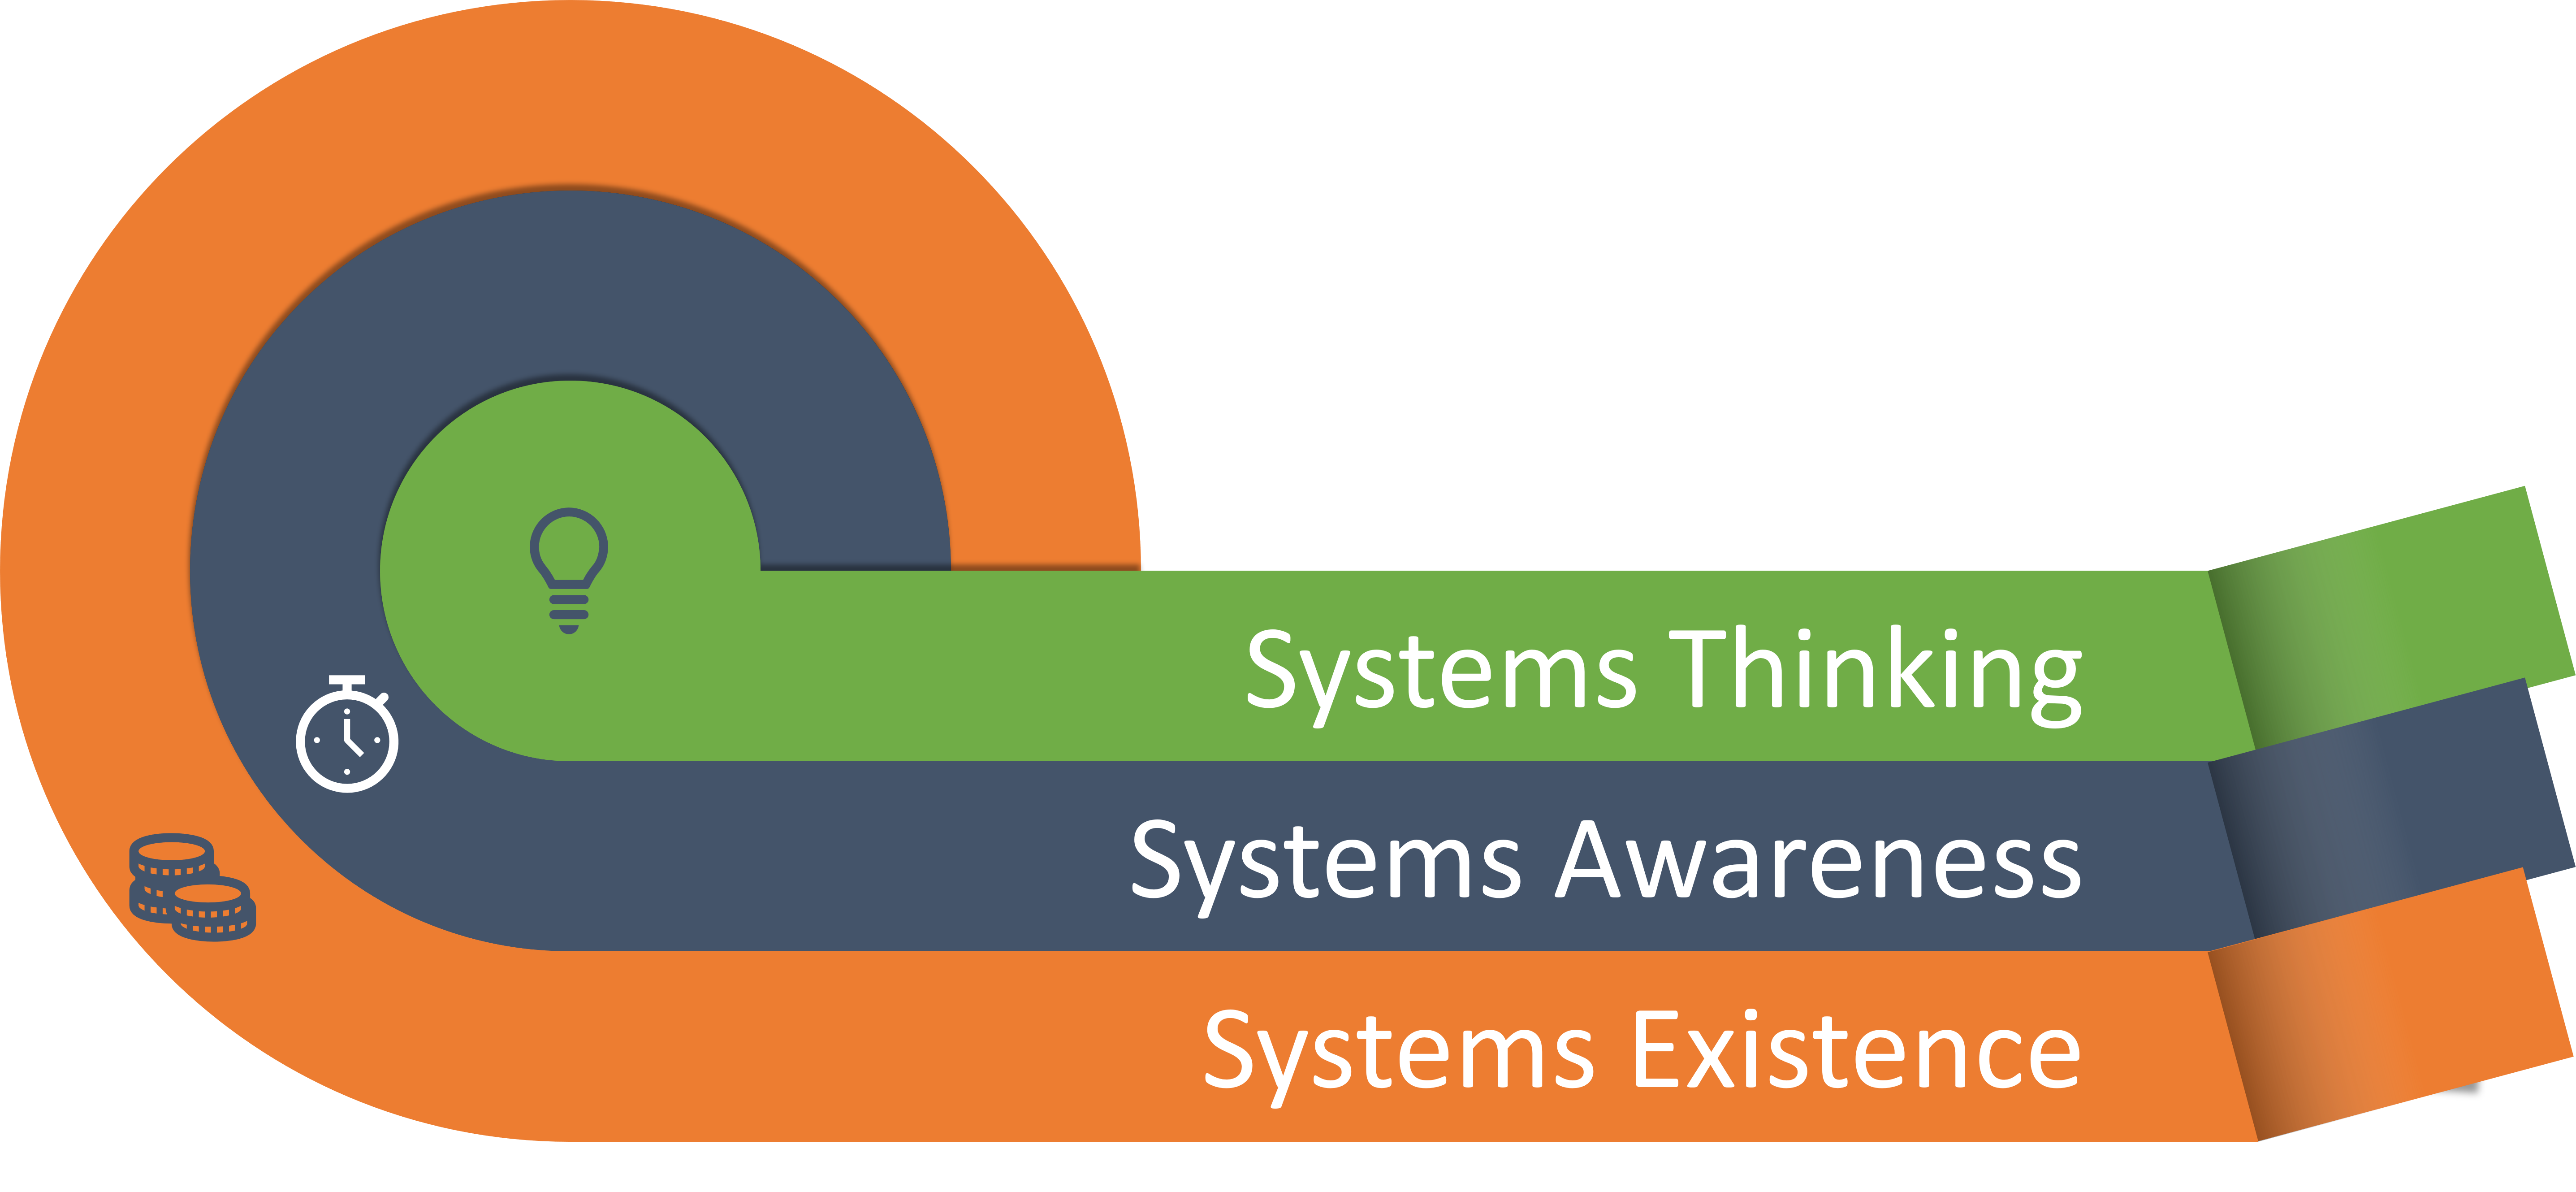
\includegraphics[width=0.9\textwidth]{systemsThinkingSnail.png}
\caption{Complete experimental setup (left) with close-up view of stage (right).}
\label{fig:systemsThinkingSnail}
\end{figure}

Figure 1.2 is conceptual in nature and self-explanatory. In science, it is argued that the only way to fully understand why a problem or element occurs and persists is to understand the parts in relation to the whole. [3] Standing in contrast to Descartes’s scientific reductionism and philosophical analysis, it proposes to view systems in a holistic manner. Consistent with systems philosophy, systems thinking concerns an understanding of a system by examining the linkages and interactions between the elements that compose the entirety of the system.

Science systems thinking attempts to illustrate that events are separated by distance and time and that small catalytic events can cause large changes in complex systems. Acknowledging that an improvement in one area of a system can adversely affect another area of the system, it promotes organizational communication at all levels to avoid the silo effect. Systems thinking techniques may be used to study any kind of system – natural, scientific, engineered, human or conceptual.

Systems thinking has been defined as an approach to problem solving, by viewing “problems” as parts of an overall system, rather than reacting to specific part, outcomes or events and potentially contributing to further development of unintended consequences. Systems thinking is not one thing but a set of habits or practices within a framework that is based on the belief that the component parts of a system can best be understood in the context of relationship with each other and with other systems, rather than in the isolation. Systems thinking focuses on cyclical rather than linear cause and effect.

\subsection{Think Globally, Act Locally}\index{Think Globally, Act Locally}

The approach adopted in this book is to recommend to globally conscious people and youth (especially STEM participants) to acquire an interest in the degree to which human designs act to modify the natural world.
\begin{enumerate}
\item More attention to design can alleviate problems revealed during operations because operational outcomes are inherent and linked to the physics of design
\item The on-line linking of individual designer’s decisions to evaluation at the system level and to stakeholder value is becoming more technically feasible. How?
\end{enumerate}

Define the system design space and partition it into the Functional domain, the Design Dependent Parameter domain, and the Optimization domain, etc.
Design Dependent Parameters (DDP’s) are suggested as the most overarching and most LINK between human designers and the human modified world. They established the design space and specific predicted and/or estimated values thereof drive design evaluation.
Design evaluation is the compass for stumbling through the design space in search of a modified world judged to be satisfactory by stakeholders.

	Add material by Kathia Laslo, PhD who directs Staybook University’s program in Leadership of Sustainable Systems . . . 
    
\subsection{Think About the End Before Beginning}\index{Think About the End Before Beginning}

From the thinking of Leonardo da Vinci
\begin{itemize}
\item WHY “To Make the World Better for People” (Retitle source here)
\item Human-made entities should be designed to satisfy human needs, wants, and objectives effectively, while minimizing system life-cycle cost as well as the intangible costs of ecological and societal impacts on the natural world
\item HOW ``Adopt and Practice Systems Thinking and Engineering''
\item A technologically based interdisciplinary process for bringing systems, products, structures, and services (human-made entities) into being
\end{itemize}

Reorient the Organization: Organization, humankind’s most important innovation, is the time-tested means for bringing human-made entities into being. While the main focus is nominally on the entities themselves, Systems Engineering embraces better strategy. Systems Engineering concentrates on what the entities do before determining what the entities are, with form following function. That is, instead of offering systems or system elements and products per se, the organizational focus should shift to designing, delivering, and sustaining functionality, a capability, or a solution.
\section{Relating Textbook STEA to STEM}\index{Relating Textbook STEA to STEM}
\section{Summary and Extensions}\index{Summary and Extensions}

Although this book focuses on the engineering of systems and on systems analysis, it would not have been intellectually prudent to begin the discussion at that level. Upon examination, it is evident that both the engineering and the analysis aspects of the focus are directed to systems. Accordingly, this chapter is devoted to helping the reader gain essential insight into systems in general, and systems thinking in particular, with orientation toward the engineering and analysis of technical systems.

System definitions, a discussion of system elements, and a high-level classification of systems provide an opening panorama. It is here that a consideration of the origin of systems provides an orientation to natural and human-made domains as an overarching dichotomy. The importance of this dichotomy cannot be overemphasized in the study and application of systems engineering and analysis. It is the suggested frame of reference for considering and understanding the interface and impact of the human-made world on the natural world and on humans. Individuals interested in obtaining an in-depth appreciation for this interface and the mitigation of environmental impacts are encouraged to read T. E. Graedel and B. R. Allenby, Industrial Ecology, 2nd ed., Prentice Hall, 2003. Also of contemporary interest is the issue of sustainability treated as part of an integrated approach to sustainable engineering by P. Stasinopoulos, M. H. Smith, K. Hargroves, and C. Desha, Whole System Design, Earthscan Publishing, 2009. These works are recommended as an extension to this chapter (as well as Chapter 16), because they illuminate and address the sensitive interface between the natural and the human-made.

This chapter is also anchored by the domains of systems science and systems engineering, beginning with the former and ending with the latter. Accordingly, it is important to recognize that at least one professional organization exists for each domain. For systems science, there is the International Society for the System Sciences (ISSS), originally named the “Society for General Systems Research.” ISSS was established at the 1956 meeting of the American Association for the Advancement of Science under the leadership of biologist Ludwig von Bertalanffy, economist Kenneth Boulding, mathematician–biologist Anatol Rapoport, neurophysiologist Ralph Gerard, psychologist James Miller, and anthropologist Margaret Mead.

The founders of the International Society for the System Sciences felt strongly that the systematic (holistic) aspect of reality was being overlooked or downgraded by the conventional disciplines, which emphasize specialization and reductionist approaches to science. They stressed the need for more general principles and theories and sought to create a professional organization that would transcend the tendency toward fragmentation in the scientific enterprise. The reader interested in exploring the field of systems science and learning more about the work of the International Society for System Sciences, may visit the ISSS website at

Most scientific and professional societies in the United States interact and collaborate with cognizant but independent honor societies. The cognizant honor society for systems engineering is the Omega Alpha Association (OAA), emerging under the motto “Think About the End Before the Beginning.” Chartered in 2006 as an international honor association, OAA has the overarching objective of advancing the systems engineering process and its professional practice in service to humankind. Among subordinate objectives are opportunities to (1) inculcate a greater appreciation within the engineering profession that every human design decision shapes the human-made world and determines its impact upon the natural world and upon people; (2) advance system design and development morphology through a better comprehension and adaptation of the da Vinci philosophy of thinking about the end before the beginning; that is, determining what designed entities are intended to do before specifying what the entities are and concentrating on the provision of functionality, capability, or a solution before designing the entities per se; and (3) encourage excellence in systems engineering education and research through collaboration with academic institutions and professional societies to evolve robust policies and procedures for recognizing superb academic programs and students. The OAA website, provides information about OAA goals and objectives, as well as the OAA vision for recognizing and advancing excellence in systems engineering, particularly in academia.

Upon completion of, the reader should have obtained essential insight into systems and systems thinking, with a focus on systems engineering and analysis. The system definitions, classifications, and concepts presented in this chapter are intended to impart a general understanding about the following:

\begin{enumerate}
\item System classifications, similarities, and dissimilarities
\item The fundamental distinction between natural and human-made systems
\item The elements of a system and the position of the system in the hierarchy of systems
\item The domain of systems science, with consideration of cybernetics, general systems theory, and systemology
\item Technology as the progenitor for the creation of technical systems, recognizing its impact on the natural world
\item The transition from the machine or industrial age to the Systems Age, with recognition of its impact upon people and society
\item System complexity and scope and the demands these factors make on engineering in the Systems Age
\item The range of contemporary definitions of systems engineering used within the profession.
\end{enumerate}

\section*{Resources for Further Exploration}
\begin{itemize}
\item \href{http://innovbfa.viabloga.com/files/Herbert_Simon___theories_of_bounded_rationality___1972.pdf}{Theories of Bounded Rationality by Herbert A. Simon}
\item \href{https://medium.com/disruptive-design/tools-for-systems-thinkers-the-6-fundamental-concepts-of-systems-thinking-379cdac3dc6a}{Tools of a Systems Thinker by Leyla Acaroglu}
\item \href{http://www.afscet.asso.fr/resSystemica/Crete02/Dyer.pdf}{Beyond Systems Design as we know it? by Gordon Dyer}
\end{itemize}

%%----------------------------------------------------------------------------------------
%	PROBLEMS
%%----------------------------------------------------------------------------------------

%% SEA CHAPTER 1 - SYSTEM SCIENCE AND ENGINEERING
% SEA Question Location in \label{sea-Chapter#-Problem#}
% ANSWERS NEED UPDATING
\begin{exercises}
    \begin{exercise}
    \label{sea-1-26}
        Describe how systems thinking differs from systems engineering.
        % What benefits could result from improving systems thinking in society?
    \end{exercise}
    \begin{solution}
        Human society is characterized by its culture. Each human culture manifests itself through the medium of technology. It takes more than a single step for society to transition from the past, to present and future technology states. A common societal response is often to make the transition and then to adopt a static pattern of behavior. A better response would be to continuously seek new but well-thought-out possibilities for advancement. Improvement in technological literacy embracing systems thinking should increase the population of individuals capable of participating in this desirable endeavor. \textbf{Reference:}
    \end{solution}
    
    \begin{exercise}
    \label{sea-1-1}
        For a system with which you are familiar, justify why it is a system according to the definition in \Cref{sec:sectors-comprising-our}.
        % Pick a system with which you are familiar and verify that it is indeed a system per the system definition given at the beginning of Section 1.1.
    \end{exercise}
    \begin{solution}
        A river system (Mississippi) is an assemblage of a watershed, tributaries, and river banks that conveys water from the continental U.S. to the Gulf of Mexico. A municipal transportation system (Chicago) is an assemblage of trains, buses, subways, etc. that transports people among many city locations. A system of organization and management (Matrix) is based on a morphology and procedure, coordinating both line and support functions. An automobile manufacturer is a combination of factories, organizations, dealerships, etc., that delivers automobiles and related support services. A home is an assemblage of land, structure, utilities, furnishings, and people that provides a supportive place to live for one or more families. \textbf{Reference:}
    \end{solution}
    
    \begin{exercise} 
    \label{sea-1-2}
        Describe the components, attributes, and relationships in the system you used in Problem \ref{sea-1-1}.
        % Name and identify the components, attributes, and relationships in the system you picked in Question 1.
    \end{exercise}
    \begin{solution}
        The major components of a home are listed in Answer 1 above. Attributes include acreage, terrain, square footage, utility capacities, styles of decorating and furnishing, personalities, and philosophies. Relationships include layout, allocation of space to people, and approaches to living together. \textbf{Reference:}
    \end{solution}
    
    \begin{exercise}
    \label{sea-1-3}
        Name any system which includes a material that transforms over the system's life cycle and identify its structural components, operating components, and flow components.
        % Pick a system that alters material and identify its structural components, operating components, and flow components.
    \end{exercise}
    \begin{solution}
        A chemica1 processing plant is composed of structural components (building, tanks, piping), operating components (pumps, valves, controls), and flow components (chemical constituents, energy, information). \textbf{Reference:}
    \end{solution}
    
    \begin{exercise} 
    \label{sea-1-4_5}
        Name any complex system and
        \begin{enumerate}[label=\alph*)]
            \item Define the hierarchy related to the system.
            \item Define the system boundaries.
        \end{enumerate}
        % Select a complex system and discuss it in terms of the hierarchy of systems.
        % Select a complex system and identify some different ways of establishing its boundaries.
    \end{exercise}
    \begin{solution}
        A dam system can be considered a complex system.
        \begin{enumerate}[label=\alph*)]
            \item todo
            \item The boundaries of a dam system can be limited to the physical dam. Alternatively, the human-modified river system, which now has a lake, can be considered a part of the dam system. The related road system, for which the dam now provides a bridge over the river, can be included. The region’s tourism service system, for which the dam system now provides an array of additional services, can be included. \textbf{Reference:}
        \end{enumerate}
    \end{solution}
    
    \begin{exercise} 
    \label{sea-1-6_7_8}
        Identify and contrast
        \begin{enumerate}[label=\alph*)]
            \item Physical versus conceptual systems.
            \item Static versus dynamic systems.
            \item Closed versus open systems.
        \end{enumerate}
        % Identify and contrast a physical and conceptual system.
        % Identify and contrast a static and a dynamic system.
        % Identify and contrast a closed and an open system.
    \end{exercise}
    \begin{solution}
        \begin{enumerate}[label=\alph*)]
            \item A physical system such as a watershed has components which manifest themselves in space and time, whereas a conceptual system such as a work breakdown structure has no physical manifestations. It is only a plan for action. Reference: Section 1.2.2 (pages 6-7).
            \item A static system such as a highway system may be contrasted with an airline system, which is a dynamic system. In the former, structure exists without activity whereas in the latter, structural components are combined with the activities of aircraft being loaded and unloaded, aircraft in flight, and controls which govern the entire operation. Reference: Section 1.2.3 (page 7).
            \item A cannon is an example of a closed system. When a cannon is fired, a one–to–one correspondence exists between the initial and final states. However, the defense contractor’s design and manufacturing organization that produced the cannon and associated projectile is an open system, with a dynamic interaction of system components. These system components must be reconfigured and adapted to cope with changing requirements. \textbf{Reference:}
        \end{enumerate}
    \end{solution}
    
    \begin{exercise} 
    \label{sea-1-15}
        For any system of the following types, name any system property
        \begin{enumerate}[label=\alph*)]
            \item Dynamic system.
            \item Steady-state system.
        \end{enumerate}
        % Give an example of a random dynamic system property and of a steady state dynamic system property.
    \end{exercise}
    \begin{solution}
        \textbf{Reference:}
    \end{solution}
    
    \begin{exercise} 
    \label{sea-1-9}
        For each of the following systems, define a unique system and describe it in terms of components, attributes, and relationships
        \begin{enumerate}[label=\alph*)]
            \item Natural system.
            \item Human-made system.
            \item Human-modified system.
        \end{enumerate}
        % Pick a natural system and describe it in terms of components, attributes, and relationships; repeat for a human-made system; repeat for a human-modified system.
    \end{exercise}
    \begin{solution}
        \begin{enumerate}[label=\alph*)]
            \item A watershed is a natural system made up of objects or components such as land, vegetation, and the watercourse; attributes such as the soil type, timber species, and the river width; and relationships such as the distribution of the attributes over the terrain. 
            \item A chemical processing plant is a human–made system with components described in Answer 3 above, attributes such as tank volume and pipe diameter, and relationships such as the flow rates and the yield of final product per energy unit utilized.
            \item A person with a pacemaker is a human-modified system with components of body parts and pacemaker parts, attributes such as body mass, diseases, attitudes, battery, controller, and electrodes, and relationships such as implantation location, rhythm, and signal strength. \textbf{Reference:}
        \end{enumerate}
    \end{solution}
    
    \begin{exercise} 
    \label{sea-1-10_11_12}
        For any Human-made system (including the system from \ref{sea-1-9})
        \begin{enumerate}[label=\alph*)]
            \item Identify the system's purpose(s) and potential metrics to present its value.
            \item Describe the system's state at any arbitrary time during operation, at least one system behavior, and an overview of the system's process.
            \item Name any two related components of the system, define the purpose of each component as it relates to the other, and the necessary attributes of the component pair such that they contribute to the purpose(s) of the entire system.
        \end{enumerate}
        % Identify the purpose(s) of the above human-made system and name some possible measures of worth.
        % For the above human-made system, describe its state at some point in time, describe one of its behaviors, and summarize its process.
        % For the above human-made system, name two components that have a relationship, identify what need each component fills for the other component, and describe how the attributes of these two components must be engineered so that the pair functions together effectively in contributing to the system’s purpose(s).
    \end{exercise}
    \begin{solution}
        \begin{enumerate}[label=\alph*)]
            \item The purposes of a chemical processing plant in a market economy are to produce one or more chemical products and possibly byproducts that can be sold at a profit while fulfilling obligations to stakeholders and the public. Measures of worth include production cost per unit volume, product quality, flexibility of product mix, benefits to stakeholders, and compatibility with society. \textbf{Reference:}
            \item During startup the state of a chemical processing plant is that pipes and vessels are filled to a certain location and empty after that location; pumps for vessels being filled are running and valves are open while other pumps are not running and valves are closed. A behavior is that when a vessel is filled, the control system turns off the pump (in a batch system) or reduces its speed (in a continuous system) and activates the next step in the process. The process is to start up, achieve the designated operational speed for each subsystem, continuously monitor the production results and make needed adjustments, and eventually shut down and clean out. \textbf{Reference:}
            \item A pump and the tank it fills have a relationship. The pump provides the material that the tank needs, while the tank provides a location where the pump can store the material it needs to deliver. The attributes of the pump must be engineered so that it can reliably move the material(s) the tank needs at an adequate rate for any given speed of overall system operation. The attributes of the tank must be engineered so that it can store the quantities of material the pump must deliver without corrosion or contamination. Thus the downstream components have the material they need to fulfill the plant’s production purpose without problems of quality or pollution. \textbf{Reference:} 
        \end{enumerate}
    \end{solution}
    
    \begin{exercise} 
    \label{sea-1-14}
        For any Human-modified system (including the system from \ref{sea-1-9}), name some positive and negative impact(s) of the modification to the natural system.
        % For a human-modified system, identify some of the ways in which the modified natural system could be degraded and some of the ways in which it could be improved.
    \end{exercise}
    \begin{solution}
        Human introduction of plant or animal species into regions where they do not naturally occur can provide the benefits of those species in the new regions, but the new species may become excessively dominant in those regions due to lack of natural enemies, crowding out or harming beneficial native species. \textbf{Reference:}
    \end{solution}
    
    \begin{exercise} 
    \label{sea-1-13}
        Give examples of each of the following
        \begin{enumerate}[label=\alph*)]
            \item First-order relationship.
            \item Second-order relationship.
            \item Redundance.
        \end{enumerate}
        % Give an example of a first-order relationship, a second-order relationship, and redundance.
    \end{exercise}
    \begin{solution}
        \begin{enumerate}[label=\alph*)]
            \item In a computer system, the power supply and system board have a first-order relationship because the system board must receive the reduced voltage produced by the power supply in order to function, and the power supply would be useless if there were no system board to perform and coordinate the computer functions. 
            \item The system board has a second-order relationship with a math coprocessor, or a video processor, or with video memory. The system board could perform the functions of these additional components, but the added components relieve the system board’s workload, thereby improving its performance.
            \item  A second power supply or a mirror image hard disk drive provide redundance, ensuring that the system board can continue receiving electrical power and the data storage function, thereby helping to assure continuation of the computer system function. \textbf{Reference:}
        \end{enumerate}
    \end{solution}
    
    \begin{exercise} 
    \label{sea-1-16}
        Name any system that operates at equilibrium and another system that degrades over time.
        % Give an example of a system that reaches equilibrium and of a system that disintegrates over time.
    \end{exercise}
    \begin{solution}
        A forest reaches equilibrium. A tree is in equilibrium until it dies, and then it disintegrates. \textbf{Reference:}
    \end{solution}
    
    \begin{exercise} 
    \label{sea-1-17}
        The United States government, for example, can be divided and described as three individual entities of the executive, legislative, and judicial branches. Create an argument for why a government of this structure should either be considered a single system or three systems.
        % Is a government with executive, legislative, and judicial branches three systems or a single system? Why?
    \end{exercise}
    \begin{solution}
        The government described is a single system because the branches thereof are functionally related. \textbf{Reference:}
    \end{solution}
    
    \begin{exercise} 
    \label{sea-1-19}
        Give any example of cybernetics and define why the example is appropriate.
        % Explain cybernetics by using an example of your choice.
    \end{exercise}
    \begin{solution}
        Cybernetics may be described and explained by considering the early mechanical version of a governor to control the revolutions per minute (RPM) of an engine. Centrifugal force, acting through a weight mechanism on the flywheel, is used to sense RPM. The outward movement of the weight against a spring acts through a link to decrease the throttle setting, thus reducing engine speed. \textbf{Reference:}
    \end{solution}
    
    \begin{exercise} 
    \label{sea-1-21}
        Do all systems at higher levels of Boulding's Hierarchy necessarily incorporate the lower levels of the hierarchy? If not, provide a specific system example.
        % Select a system at one of the higher levels in Boulding’s hierarchy and describe if it does or does not incorporate the lower levels.
    \end{exercise}
    \begin{solution}
        \textbf{Reference:}
    \end{solution}
    
    \begin{exercise} 
    \label{sea-1-22}
        Describe a novel system that may be necessary for society 50 to 100 years in the future and
        \begin{enumerate}[label=\alph*)]
            \item Define the system requirements.
            \item Define the system objectives.
        \end{enumerate}
        % Identify a societal need, define the requirements of a system that would fill that need, and define the objective(s) of that system.
    \end{exercise}
    \begin{solution}
        Efficient transportation system to the Moon and/or Mars. \textbf{Reference:}
    \end{solution}
    
    \begin{exercise} 
    \label{sea-1-25}
        For the system described in Question \ref{sea-1-22}
        \begin{enumerate}[label=\alph*)]
            \item Identify factors which led to the need for a new system.
            \item Identify other societal factors which may evolve in parallel and lead to other changes or innovations.
        \end{enumerate}
        % Name some of the factors driving technological advancement and change.
    \end{exercise}
    \begin{solution}
        \begin{enumerate}[label=\alph*)]
            \item Factors driving technological change include attempts to respond to unmet current needs and attempts to perform ongoing activities in a more efficient and effective manner, as well as social factors, political objectives, ecological concerns, and the desire for environmental sustainability. \textbf{Reference:}
            \item todo
        \end{enumerate}
    \end{solution}
    
    \begin{exercise} 
    \label{sea-1-23}
        Compare and contrast systemology and synthesis.
        % What are the similarities of systemology and synthesis?
    \end{exercise}
    \begin{solution}
        Both systemology and synthesis produce systems. Systemology produces a system of processes by which systems are brought into being and carried through the life cycle. Synthesis produces any kind of system. Synthesis is a part of systemology and also a product of systemology. \textbf{Reference:}
    \end{solution}
    
    \begin{exercise} 
    \label{sea-1-24}
        Classify a technical system.
        % What difficulty is encountered in attempting to classify technical systems?
    \end{exercise}
    \begin{solution}
        The phrase “technical system” is used to represent all types of human–made artifacts, including engineered products and processes. Classifying a technical system is generally difficult, because a technical system derives its inputs from several disciplines or fields which may be very different from one another. \textbf{Reference:}
    \end{solution}
    
    \begin{exercise} 
    \label{sea-1-27}
        Compare and contrast the attributes of the Machine (Industrial) Age and the Systems Age.
        % Identify the attributes of the Machine or Industrial Age and the Systems Age.
    \end{exercise}
    \begin{solution}
        Attributes of the Machine Age are determinism, reductionism, physical, cause and effect, and closed system thinking. The Systems Age has attributes of open systems thinking, expansionism, human–machine interfacing, automation, optimization, and goal orientation. \textbf{Reference:}
    \end{solution}
    
    \begin{exercise} 
    \label{sea-1-28}
        Identify key differences between synthetic and analytical thinking. Is one method of thinking always preferable? Why or why not?
        % Explain the difference between analytic and synthetic thinking.
    \end{exercise}
    \begin{solution}
        Analytic thinking seeks to explain the whole based on explanations of its parts. Synthetic thinking explains something in terms of its role in a larger context. \textbf{Reference:}
    \end{solution}
    
    \begin{exercise} 
    \label{sea-1-29}
        What challenges make the Systems Age unique from other periods of human evolution?
        % What are the special engineering requirements and challenges in the Systems Age?
    \end{exercise}
    \begin{solution}
        The special engineering requirements of the Systems Age are those which pertain to integration, synthesis, simulation, economic analysis, and environmental concerns, along with the necessity to bring the classical engineering disciplines to bear on the system under development through collaboration. \textbf{Reference:}
    \end{solution}
    
    \begin{exercise} 
    \label{sea-1-30}
        Compare and contrast systems engineering with other engineering disciplines.
        % What are the differences (and similarities) between systems engineering and the traditional engineering disciplines?
    \end{exercise}
    \begin{solution}
        Both systems engineering and the traditional engineering disciplines deal with technology and technical (human-made) entities. The focus of traditional engineering is on technical design of the entities in human-made systems, whereas systems engineering concentrates on what the entities are intended to do (functional design) before determining what the entities are. Traditional engineering focuses on technical performance measures, whereas systems engineering considers all requirements of the client, system owner, and/or the user group, as well as the effects on related systems. Traditional engineering focuses on designing products for their operational uses, whereas systems engineering considers all the life cycles of the systems that include its products. Traditional engineering tends to proceed from the bottom-up, whereas systems engineering favors a top-down approach. Traditional engineering favors analytic thinking while systems engineering favors synthetic thinking. Traditional engineering applies the skills of particular engineering disciplines to problems, whereas systems engineering defines problems before determining what disciplines are needed. Systems engineering provides methodologies that facilitate effective teamwork among not only the traditional engineering disciplines, but also among other technical as well as social disciplines. \textbf{Reference:}
    \end{solution}
    
    \begin{exercise} 
    \label{sea-1-32}
        Identify a system which required an interdisciplinary approach to develop \textit{or} to implement. What disciplines were required and why?
        % Give an example of a problem requiring an interdisciplinary approach and identify the needed disciplines.
    \end{exercise}
    \begin{solution}
        The problem of predicting the availability and amount of oil and natural gas from a certain geological region, which might be available to refineries and power plants in another region in future time periods, requires the disciplines of geology, petroleum engineering, regional planning, civil engineering, ecological science, transportation engineering, and economics. The validity of the prediction depends largely upon the proper utilization and interpretation of findings by the relevant disciplines and their domains of inquiry. \textbf{Reference:}
    \end{solution}
    
    \begin{exercise} 
    \label{sea-1-33}
        Identify an interdiscipline and the disciplines from which it was derived.
        % Name an interdiscipline and identify the disciplines from which it was drawn.
    \end{exercise}
    \begin{solution}
        Systems engineering is an interdiscipline (sometimes called a multidiscipline or transdiscipline) drawn mainly from the engineering disciplines, but also from mathematics, operations research, systemology, project management, and increasingly, other fields. \textbf{Reference:}
    \end{solution}
    
    \begin{exercise} 
    \label{sea-1-35_36_38}
        For the following organizations, summarize their mission statements
        \begin{enumerate}[label=\alph*)]
            \item \href{http://isss.org/}{International Society for the Systems Sciences}
            \item \href{https://www.incose.org/}{International Council on Systems Engineering}
            \item \href{https://omegalpha.org/}{Omega Alpha Association}
        \end{enumerate}
        % Go to the website for ISSS given in Section 1.7 and summarize the goal of the society.
        % Go to the website for INCOSE given in Section 1.7 and summarize the goals of the council.
        % Go to the website for OAA and compare this honor society with one that you are familiar with.
    \end{exercise}
    \begin{solution}
        \begin{enumerate}[label=\alph*)]
            \item Independent exercise. Visit http://isss.org/
            \item Independent exercise. Visit https://www.incose.org/
            \item Independent exercise. Visit https://omegalpha.org/
        \end{enumerate}
    \end{solution}
    
    \begin{exercise} 
    \label{sea-1-37}
        Explain how the goals of ISSS and INCOSE differ.
        % Contrast the goals of ISSS and INCOSE as given in Section 1.7 or on the web.
    \end{exercise}
    \begin{solution}
        Independent exercise. Refer to the solution of \ref{sea-1-35_36_38}.
    \end{solution}
\end{exercises}
% SKIPPED
% sea-1-18 Identify a system-of-systems whose analysis could yield insights not available by separately analyzing the individual systems of which it is composed.
% sea-1-20 Give a system example at any five of the levels in Boulding’s hierarchy.
% sea-1-31 Given the recommendations in Educating the Engineer of 2020, what should be added to the curriculum with which you are familiar?
% sea-1-34 Write your own (preferred) definition of systems engineering.


\chapterimage{wireFrame.jpg} % Chapter heading image
\chapter{SCIENTIFIC THINKING AND KNOWLEDGE}\label{chap:02}

In recent decades, humans have begun to understand the underlying structure and characteristics of natural and human-made systems in a scientific way. Chapter One emphasized the human-modified world as primary evidence of the importance of drawing upon each system category.

Some system definitions and system science concepts are presented to provide a basis for the study of systems engineering and analysis. They include the definitions of system characteristics, a classification of systems into various types, consideration of the current state of systems science, and a discussion of the transition to the Systems Age. Finally, the chapter presents technology and the nature and role of engineering in the Systems Age and ends with an account of the development of systems thinking to date with extension beyond the world we know today.

%%----------------------------------------------------------------------------------------
%	CHAPTER CONTENT
%%----------------------------------------------------------------------------------------

\section{Human Curiosity and Inquiry}\index{Human Curiosity and Inquiry}

A major part of human nature is the curiosity of people. Curiosity leads to inquiry, and inqooint to increased understanding. “The more you learn, the more acutely aware you become of your ignorance.”

How do we know about the world in which we live – or reality, for that matter?  Where does our knowledge about it come from?  The attempt to answer these questions lead to epistemology, the branch of philosophy dealing with the origin, scope, and validity of human knowledge.

In the epistemological debate, there are two archetypal and actually diametrically opposed concepts: empiricism and rationalism. Empiricism claims that sensory experience (observation) is man’s main (or even sole) source of knowledge, which rationalism claims that his knowledge stems from human reason.

Hardly anyone would deny that there is knowledge that comes to us from sensory experience. Take, for instance, the knowledge that water freezes at zero degrees Celsius. It actually takes observation(s) to acquire such knowledge.

However, in the field of science, which formulates knowledge that applies universally, irrespective of time and place, rationalism holds that empirical knowledge gained through sensory experience doesn’t have the same validity as knowledge deduced from reasoning.
    
\subsection{Human Nature to Inquire}\index{Human Nature to Inquire}

The branches of contemporary science associated with the study of human nature include anthropology, sociology, sociobiology, and psychology, particularly evolutionary psychology, which studies sexual selection in human evolution, as well as developmental psychology. The ``nature versus nurture'' debate is a broadly inclusive and well-known instance of discussion about human nature in the natural science.

This common phrase refers to the distinguishing characteristics – including ways of thinking, feeling, and acting – which humans tend to have naturally, independently of the influence of culture. The questions of what these characteristics are, how fixed they are, and what causes them are amongst the oldest and most important questions in philosophy and science. These questions have particularly important implications in ethics, politics, and theology. This is partly because human nature can be regarded as both a source of norms of conduct of ways of life, as well as presenting obstacles or constraints on living a good life. The complex implications of such questions are also dealt with in art and literature, the question of what it is to be human.

The concept of nature as a standard by which to make judgments was a basic presupposition in Greek philosophy. Specifically, ``almost all'' classical philosophers accepted that a good human life is a life in accordance with nature. (Notions and concepts of human nature from China, Japan, or India are not taken up in the present discussion.)

On this subject, the approach of Aristotle – sometimes considered to be a teleological approach – came to be dominant by late classical and medieval times. This approach understands human nature in terms of final and formal causes. In other words, nature itself (or a nature-creating divinity) has intentions and goals, similar somehow to human intentions and goals, and one of those goals is humanity living naturally. Such understandings of human nature see this nature as an ``idea'', or ``form'' of a human. By this account, human nature really causes humans to become what they become, and so it exists somehow independently of individual humans. This in turn has sometimes been understood as also showing a special connection between human nature and divinity.

However, the existence of this invariable human nature is a subject of much historical debate, continuing into modern times. Against this idea of a fixed human nature, the relative malleability of man has been argued especially strongly in recent centuries – firstly by early modernists such as Thomas Hobbes and Jean-Jacques Rousseau. In Rousseau’s Emile, or On Education, Rousseau wrote: “We do not know what our nature permits us to be.”  Since the early 19th century, thinkers such as Hegel, Marx, Kierkegaard, Nietzsche, Sartre, structuralists, and postmodernists have also sometimes argued against a fixed or innate human nature.

Charles Darwin’s theory of evolution has changed the nature of the discussion, confirming the fact that mankind’s ancestors were not like mankind today. Still more recent scientific perspectives – such as behaviorism, determinism, and the chemical model within modern psychiatry and psychological – claim to be neutral regarding human nature. (As in much of modern science, such disciplines seek to explain with little or no recourse to metaphysical causation.)  They can be offered to explain human nature’s origins and underlying mechanisms, or to demonstrate capacities for change and diversity which would arguably violate the concept of a fixed human nature.

\subsection{How Do We Know?}\index{How Do We Know?}

The notion of ``letting the facts speak for themselves'' without taking recourse to a theory is nonsensical. Mises was aware the people’s ``reasoning may be faulty and the theory incorrect; but thinking and theorizing are not lacking in any action.''

How do we know, and how can we make sure, that we employ a correct theory?  Fortunately, in social science a satisfactory answer can be given to these questions by taking recourse to a priori theory – meaning propositions that provide true knowledge about reality, and whose truth value can be validated independent of experience.

To explain, we have to turn briefly to the Prussian philosopher Immanuel Kant (1724-1804) and his groundbreaking The Critique of Pure Reason (1781). A central outcome of what Kant called transcendental investigation in his discovery of so-called a priori synthetic judgements.
    
\subsection{\textit{A Priori} Theory}\index{\textit{A Priori} Theory}

A priori denotes a proposition (a declarative statement) expressing knowledge that is acquired prior to, or independently from, experience. In contrast, a posteriori denotes knowledge that is acquired through and on the basis of experience.

A synthetic judgment refers to knowledge that is not contained in the subject matter. An example is ``All bodies are heavy.''  Here, the predicate ``heavy'' conveys knowledge that goes beyond the mere concept of ``body'' in general. A synthetic judgment thus yields new knowledge about the subject matter.

Analytical judgments repeat what the concept of the subject matter already presupposes. An example is ``All bodies are extended.''  In order to know that bodies are extended one does not need experience, as this information is already in the concept of ``bodies.''

One would expect that analytical judgements are a priori, while synthetic judgements are posteriori. However, Kant claims that there exist a priori synthetic judgements – knowledge that neither merely repeats the meaning of the concept under review nor requires experience to say something new about the subject matter.

How can a priori synthetic judgements be identified?  According to Kant, a proposition must meet two requirements in order to qualify as an a priori synthetic judgement. First, it must not result from experience, but from reasoning. Second, it cannot be denied without causing an intellectual contradiction.

A priori theory offers an approach for reviewing, criticizing, and possibly revising commonly held theoretical explanations of historical events. When (re)viewed from point of a priori theory, what can be said about the two independent observations?

A priori theory provides true knowledge about the outer world, and the truth of knowledge derived from a priori theory can be validated independent of sensory experience.

By no means less important, a priori knowledge trumps empirical knowledge: ``A proposition of an aprioristic theory can never be refuted by experience.''

Praxeology, the a priori science of human action, and, more specifically, it’s up to now bed-developed part, economics, provides in its field a consummate interpretation of past events recorded and a consummate anticipation of the effects to be expected from future actions of a definite kind.

An a priori theorist can thus decide in advance (that is, without engaging in social experimentation, or testing, for that matter) whether or not a given action – policy measure – can bring about the promised effects.

For instance, we know a priori that issuing flat money does not create economic prosperity, that tax- or debt-financed government spending does not improve society’s material well-being, and that these measures are actually economically harmful.

A priori theory is an intellectually powerful defense against promises made by false theory and its detrimental (even disastrous) economic consequences if put into practice. Students of social sciences should therefore be increasingly encouraged to engage in a priori theory.

In his seminal book Systems Thinking, Systems Practice, Peter Checkland defined systems thinking as thinking about the world through the concept of “system.”  This involves thinking in terms of processes rather than structures, relationships rather than components, interconnections rather than separation. The focus of the inquiry is on the organization and the dynamics generated by the complex interaction of systems embedded in other systems and composed by other systems.
\section{Scientific Thinking in Antiquity}\index{Scientific Thinking in Antiquity}

The application of knowledge gained from the scientific method concerns prediction of the future. If X happens then Y will happen. That is the utility. Y may include probability functions.

\subsection{Classic Greek Philosophy}\index{Classic Greek Philosophy}

Philosophy in classical Greece is the ultimate origin of the western conception of the nature of a thing. According to Aristotle, the philosophical study of human nature itself originated with Socrates, who turned philosophy from study of the heavens to study of the human things.

Socrates is said to have studied the question of how a person should best live, but he left no written works. It is clear from the works of his students Plato and Xenophon, and also by what was said about him by Aristotle (Plato’s student), that Socrates was a rationalist and believed that the best life and the life most suited to human nature involved reasoning. The Socratic school was the dominant surviving influence in philosophical discussion in the Middle Ages, amongst Islamic, Christian, and Jewish philosophers.

The human soul in the works of Plato and Aristotle has a divided nature, divided in a specifically human way. One part is specifically human and rational, and divided into a part which is rational on its own, and a spirited part which can understand reason. Other parts of the soul are home to desires or passions similar to those found in animals. In both Aristotle and Plato, spiritedness (thumos) is distinguished from the other passions (epithumiai). The proper function of the ``rational'' was to rule the other parts of the soul, helped by spiritedness. By this account, using one’s reason is the best way to live, and philosophers are the highest types of human.

Aristotle – Plato’s most famous student – made some of the most famous and influential statements about human nature. In his works, apart from using a similar scheme of a divided human soul, some clear statements about human nature are made:
\begin{enumerate}
\item Man is a conjugal animal, meaning an animal which is born to couple when an adult, thus building a household (oikos) and, in more successful cases, a clan or small village still run upon patriarchal lines.
\item Man is a political animal, meaning an animal with an innate propensity to develop more complex communities the size of a city or town, with a division of labor and law-making. This type of community is different in a kind from a large family and requires the special use of human reason.
\item Man is mimetic animal. Man loves to use his imagination (and not only to make laws and run town councils). He says ``we enjoy looking at accurate likenesses of things which are themselves painful to see, obscene beasts, for instance, and corpses.''  And the ``reason why we enjoy seeing likenesses is that, as we look, we learn and infer what each is, for instance, ‘that is so and so.’''
\end{enumerate}
For Aristotle, reason is not only what is most special about humanity compared to other animals, but it is also what we were meant to achieve at our best. Much of Aristotle’s description of human nature is still influential today. However, the particular teleological idea that humans are ``meant'' or intended to be something has become much less popular in modern times.

For the Socratics, human nature, and all natures, are metaphysical concepts. Aristotle developed the standard presentation of this approach with his theory of four causes. Every living thing exhibits four aspects or ``causes'': matter, form, effect, and end. For example, an oak tree is made of plant cells (matter), grew from an acorn (effect), exhibits the nature of oak trees (form), and grows into a fully mature oak tree (end). Human nature is an example of a formal cause, according to Aristotle. Likewise, to become a fully actualized human being (including fully actualizing the mind) is our end. Aristotle (Nicomachean Ethics, Book X) suggests that the human intellect is ``smallest in bulk'' but the most significant part of the human psyche, and should be cultivated above all else. The cultivation of learning and intellectual growth of the philosopher, which is thereby also the happiest and least painful life.

Although this new realism applied to the study of human life from the beginning – for example, in Machiavelli’s works – the definitive argument for the final rejection of Aristotle was associated especially with Francis Bacon. Bacon sometimes wrote as if he accepted the traditional four causes (``It is a correct position that ``true knowledge is knowledge by causes.'' And causes again are not improperly distributed into kinds: the material, the formal, the efficient, and the final.'') but he adapted these terms and rejected one of the three:

``But of these the final cause rather corrupts than advances the sciences, except such as have to do with human action. The discovery of the formal is despaired of. The efficient and the material (as they are investigated and received, that is, as remote causes, without reference to the latent process leading to the form) are but slight and superficial, and contribute little, if anything, to true and active science.''

This line of thinking continued with Rene Descartes, whose new approach returned philosophy or science to its pre-Socratic focus upon non-human things. Thomas Hobbes, then Grammatist Vico, and David Hume all claimed to be the first to properly use a modern Baconian scientific approach to human things.

Hobbes famously followed Descartes in describing humanity as matter in motion just like machines. He also very influentially described man’s natural state (without science and artifice) as one where life would be “solitary, poor, nasty, brutish, and short.”  Following him, John Locke’s philosophy of empiricism also saw human nature as a tabula rasa. In this view, the mind is at birth a “blank slate” without rules, so data are added, and rules for processing them are formed solely by our sensory experiences.

Jean-Jacques Rousseau pushed the approach of Hobbes to an extreme and criticized it at the same time. He was a contemporary and acquaintance of Hume, writing before the French Revolution and long before Darwin and Freud. He shocked Western civilization with his Second Discourse by proposing that humans had once been solitary animals, without reason or language or communities, and had developed these things due to accidents of pre-history. (This proposal was also less famously made by Giambattista Vico.)  In other words, Rousseau argued that human nature was not only not fixed, but not even approximately fixed compared to what had been assumed before him. Humans are political, and rational, and have language now, but originally, they had none of these things. This in turn implied that living under the management of human reason might not be a happy way to live at all, and perhaps there is no ideal way to live. Rousseau is also unusual in the extent to which he took the approach of Hobbes, asserting that primitive humans were not even naturally social. A civilized human is therefore not only imbalanced and unhappy because of the mismatch between civilized life and human nature, but unlike Hobbes, Rousseau also became well known for the suggestion that primitive humans had been happier, “noble savages.”

Rousseau’s conception of human nature has been seen as the origin of many intellectual and political developments of the 19th and 20th centuries. He was an important influence upon Kant, Hegel, and Marx, and the development of German idealism, historicism, and romanticism.

What human nature did entail, according to Rousseau and the other modernists of the 17th and 18th centuries, were animal-like passions that led humanity to develop language and reasoning, and more complex communities (or communities of any kind, according to Rousseau).

In contrast to Rousseau, David Hume was a critic of the oversimplifying and systematic approach of Hobbes, Rousseau, and some others whereby, for example, all human nature is assumed to be driven by variations of selfishness. Influenced by Hutcheson and Shaftesbury, he argued against oversimplification. On the one hand, he accepted that, for many political and economic subjects, people could be assumed to be driven by such simple selfishness, and he also wrote of some of the more social aspects of ``human nature'' as something which could be destroyed, for example if people did not associate in just societies. On the other hand, he rejected what he called the ``paradox of the sceptics'', saying that no politician could have invented words like \textit{honorable}, \textit{shameful}, \textit{lovely}, \textit{odious}, \textit{noble}, and \textit{despicable}, unless there was not some natural ``original constitution of the mind.''

Hume – like Rousseau – was controversial in his own time for his modernist approach, following the example of Bacon and Hobbes, of avoiding consideration of metaphysical explanations for any type of cause and effect. He was accused to being an atheist. He wrote:

``We needn’t push our researches so far as to ask `Why do we have humanity, i.e. a fellow-feeling with others?'  It’s enough that we experience this as a force in human nature. Our examination of causes must stop somewhere.''

After Rousseau and Hume, the nature of philosophy and science changed, branching into different disciplines and approaches, and the study of human nature changed accordingly. Rousseau’s proposal that human nature is malleable became a major influence upon international revolutionary movements of various kinds, while Hume’s approach has been more typical in Anglo-Saxon countries, including the United States.

\subsection{What Man Has Built}\index{What Man Has Built}

Humanity (???) Twentieth Century, more than our ancestors, must attempt to understand the varied peoples with whom he shares an increasingly small planet. To reach this understanding he needs to know the cultures which molded other people’s outlook, the history that carried them to this point.

How to select the civilizations that must be examined in a limited series of books on the history of the world’s cultures?  That is the subject of Jaques Barzun’s introduction to the Time-Life series entitled The Great Ages of Man. Mr. Barzun, Dean of Faculties and Provost of Columbia University, is one of the pre-eminent cultural historians of this generation. He describes how the “revolution … in our conception of humanity” wrought by the emergence of “dozens of new peoples, new states, and new pasts” has made essential the realization that “nothing human is alien.”

In explaining the criteria for the selection of historic cultures examined in this series, he also suggests the path that present-day cultures may follow in the future.

At the end of this introductory booklet is a comprehensive chronological chart. This shows the meaningful relationships of great cultures the world over – in time, in place, and in the interpenetrations discussed by Dean Barzum. A number of these cultures provide the subject matter for volumes in this series. This overall chart will be found useful in connection with each book; in addition, each book includes an appropriate segment from the chart. THE EDITORS OF TIME-LIFE BOOKS (1965 Time Inc.)
\section{Contemporary Scientific Thinking}\index{Contemporary Scientific Thinking}

The word ``science'' is derived from the Latin word Scientia, which is knowledge based on demonstrable and reproducible data, according to the Merriam-Webster Dictionary. True to this definition, science aims for measurable results through testing and analysis. Science is based on fact, not opinion or preferences. The process of science is designed to challenge ideas through research. One important aspect of the scientific process is that it focuses only on the natural world, according to the University of California. Anything that is based on faith alone or is considered supernatural does not fit into the definition of science.

\subsection{Deductive and Inductive Reasoning}\index{Deductive and Inductive Reasoning}

During the scientific process, deductive reasoning is used to reach a logical true conclusion. Another type of reasoning, inductive, is also used. Often, deductive reasoning and inductive reasoning are confused. It is important to learn the meaning of each type of reasoning so that proper logic can be identified.

Deductive Reasoning. is a basic form of valid reasoning. Deductive reasoning, or deduction, starts out with a general statement, or hypothesis, and examines the possibilities to reach a specific, logical conclusion, according to the University of California. The scientific method uses deduction to test hypothesis and theories. ``In deductive interference, we hold a theory and based on it we make a prediction of its consequences. That is, we predict what the observations should be if the theory were correct. We go from the general – the theory – to the specific – the observations,'' said Dr. Sylvia Wassertheil-Smoller, a researcher and professor emerita at Albert Einstein College of Medicine.

In deductive reasoning, if something is true of a class of things in general, it is also true for all members of that class. For example, ``All men are mortal. Harold is a man. Therefore, Harold is mortal.''  For deductive reasoning to be sound, the hypothesis must be correct. It is assumed that the premises, ``All men are mortal'' and ``Harold is a man'' are true. Therefore, the conclusion is logical and true.

According to the University of California, deductive inference conclusions are certain provided the premises are true. It’s possible to come to a logical conclusion even if the generalization is not true. If the generalization is wrong, the conclusion may be logical, but it may also be untrue. For example, the argument, ``All bald men are grandfathers. Harold is bald. Therefore, Harold is a grandfather,'' is valid logically but it is untrue because the original statement is false.

A common form of deductive reasoning is the syllogism, in which two statements – a major premise and a minor premise – reach a logical conclusion. For example, the premise ``Every A is B'' could be followed by another premise, ``This C is A.''  Those statements would lead to the conclusion ``This C is B.'' Syllogisms are considered a good way to test deductive reasoning to make sure the argument is valid.

Inductive Rreasoning. is the opposite of deductive reasoning. Inductive reasoning makes broad generalizations from specific observations. ``In inductive inference, we go from the specific to the general. We make many observations, discern a pattern, make a generalization, and infer an explanation or a theory.'' Wassertheil-Smoller told Live Science. ``In science there is a constant interplay between inductive inference (based on observations) and deductive inference (based on theory), until we get closer and closer to the `truth', which we can only approach but not ascertain with complete certainty.''

Even if all of the premises are true in a statement, inductive reasoning allows for the conclusion to be false. Here’s an example: ``Harold is a grandfather. Harold is bald. Therefore all grandfathers are bald.''  The conclusion does not follow logically from the statements.

Inductive reasoning has its place in the scientific method. Scientists use it to form hypothesis and theories. Deductive reasoning allows them to apply the theories to specific situations.

Abductive Reasoning. Another form of scientific reasoning that doesn’t fit in with inductive or deductive reasoning is abductive. Abductive reasoning usually starts with an incomplete set of observations and proceeds to the likeliest possible explanation for the group of observations, according to Butte College. It often entails making an educated guess after observing a phenomenon for which there is no clear explanation.

Abductive reasoning is useful for forming hypotheses to be tested. Abductive reasoning is often used by doctors who make a diagnosis based on test results and by jurors who made decisions based on the evidence presented to them.

Systems Science. Systems sciences are scientific disciplines partly based on systems thinking such as chaos theory, complex systems, control theory, cybernetics, sociotechnical systems theory, systems biology, systems ecology, systems psychology and the already mentioned systems dynamics, systems engineering, and systems theory.

Systems being involves embodying a new consciousness, and expanded sense of self, a recognition that we cannot survive alone, that a future that works for humanity needs also to work for other species and the planet. It involves empathy and love for the greater human family and for all our relationships - plants and animals, earth and sky, ancestors and descendants, and the many peoples and beings that inhabit our Earth. This is the wisdom of many indigenous cultures around the world, this is part of the heritage that we have forgotten and we are in the process of recovering.

Systems being and systems living brings it all together: linking head, heart and hands. The expression of systems being is an integration of our full human capacities. It involves rationality with reverence to the mystery of life, listening beyond words, sensing with our whole being, and expressing our authentic self in every moment of our life. The journey from systems thinking to systems being is a transformative learning process of expansion of consciousness - from awareness to embodiment.

Kathia Laslo, Ph.D., directs Saybrook University’s program in Leadership of Sustainable Ssytems.
NOTE: This post is an excerpt from the plenary presentation “Beyond Systems Thinking: The role of beauty and love in the transformation of our world” by Dr. Karla Lazslo at the 55th Meeting of the International Society for the Systems Sciences at the University of Hull, U.K., on July 21, 2014.

Systems thinking is the process of understanding how things influence one another within a whole. In nature, systems thinking examples include ecosystems in which various elements such as air, water, movement, plants, and animals work together to survive or perish. In organizations, systems consist of people, structures, and processes that work together to make an organization healthy or unhealthy.

Systems thinking has been defined as an approach to problem solving, by viewing “problems” as parts of an overall system, rather than reacting to specific part, outcomes or events and potentially contributing to further development of unintended consequences. Systems thinking is not one thing but a set of habits and practices within a framework that is based on the belief that the component parts of a system can best be understood in the context of relationships with each other and with other systems, rather than in isolation. Systems thinking focuses on cyclical rather than linear cause and effect.

In science systems, it is argued that the only way to fully understand why a problem or element occurs and persists is to understand the parts in relation to the whole. Standing in contrast to Descartes’s scientific reductionism and philosophical analysis, it proposes to view systems in a holistic manner. Consistent with systems philosophy, systems thinking concerns an understanding of a system by examining the linkages and interactions between the elements that compose the entirety of the system.

Science systems thinking attempts to illustrate that events are separated by distance and time and that small catalytic events can cause large changes in complex systems. Acknowledging that an improvement in one area of a system can adversely affect another area of the system, it promotes organizational communication at all levels in order to avoid the silo effect. Systems thinking techniques may be used to study any kind of system – natural, scientific, engineered, human, or conceptual.

\subsection{The Scientific Method}\index{The Scientific Method}

The prevailing scientific thinking in Western cultures today is naturalism. It is assumed that there is no God and that the entire universe can be explained on the basis of physical realities plus time and chance. It is assumed that the laws of physics have never changed and that conditions have been uniform in the past so that recent observations can be compiled and conclusions drawn about the past by simply looking back in time. The scientific method is mostly limited to the study of measurable entities in the physical world. Results should be verifiable by others.

Figure 2.1 Here (New)

\begin{enumerate}
\item Basic Assumptions include underlying philosophy, for example is there an outside intelligence operating, or is the system closed depending only on internal known laws. Are the laws of nature constant everywhere?  Were conditions in the past the same as they are now?  What initial conditions are assumed?  Science does not and cannot take place in a vacuum – an underlying world-view or philosophy is presupposed.
\item The hypothesis is a proposed explanation for an observed phenomenon. The simpler the explanation that fits the facts, the better, known as Occam’s razor. Science assumes we live in a universe. That is, the laws of physics are the same everywhere and, furthermore, they do not vary erratically – nature is predictable, and the universe is rational.
\item If the hypothesis does not explain the known facts or the new data, it is important to carefully examine the initial conditions to if one or more of them is incorrect or suspect. Wrong assumptions a long time ago that have not been challenged cause the weight of tradition to prevail – until there are overwhelming reasons for changing the prevailing scientific paradigm.
‘Science is the only self-correcting human institution, but it is also a process that progresses only by showing itself to be wrong.’ – Alan Sandage
\item Data inputs include measurements and observations. These are systematized and subjected to statistical scrutiny whenever possible.
\item When a theory has been found that seems to the known facts, the theory is then extended into the unknown to make predictions. These predictions are then tested by seeking additional data, exceptions, or confirmations.
\item A new scientific theory or model remains in vogue until new facts are found that contradict the model or whenever a better theory comes along.
\end{enumerate}

When conducting research, scientists use the scientific method to collect measurable, empirical evidence in an experiment related to a hypothesis (often in the form of an if/then statement), the results aiming to support or contradict a theory.
The steps of the scientific method must include: 
Make an observation or observations.
Ask questions about the observations and gather information.

\begin{enumerate}
\item Form a hypothesis – a tentative description of what’s been observed, and make predictions based on that hypothesis.
\item Test the hypothesis and predictions in an experiment that can be reproduced.
\item Analyze the data and draw conclusions; accept or reject the hypothesis or modify the hypothesis if necessary.
\end{enumerate}

Reproduce the experiment until there are no discrepancies between observations and theory. ``Replication of methods and results is an essential step in the scientific method.''

Some key underpinnings to the scientific method are:
\begin{itemize}
\item The hypothesis must be testable and falsifiable, according to North Carolina State University. Falsifiable means that there must be a possible negative answer to the hypothesis.
\item Research must involve deductive reasoning and inductive reasoning. Deductive reasoning is the process of using true premises to reach a logical true conclusion while inductive reasoning takes the opposite approach.
\item An experiment should include a dependent variable (which does not change) and an independent variable (which does change).
\item An experiment should include an experimental group and a control group. The control group is what the experimental group is compared against.
\end{itemize}

Gaining new insights into the nature of systems, Hillary Sillitto, 

Several INCOSE members participated in the IFSR Conversation held April 2018 in Linz, Austria. This article is a report on some interesting results coming out of this activity. INCOSE joined the International Federation for Systems Research in 2012, interfacing through the Systems Science Working Group, and INCOSE members have participated in each Conversation since the year we joined.

One of the major activities of the International Federation for Systems Research (IFSR) is the ``conversation'' held every two years in Linz, Austria, where several teams of typically 6-8 people spend a week discussing different current issues in systems research. The format is a ``conversation'' or ``systemic inquiry'' rather than a conference, and the teams spend most of the time in their own group, exploring their specific topic and attempting to achieve new insights by integrating the different perspectives and worldviews of the different team members. 

Over forty organizations are currently IFSR members. Some are more active than others, and the Conversation this year involved people from INCOSE, ISSS, ASC (American Society of Cybernetics), the IFSR itself, and one representative from the System Dynamics Society (SDS).

The 2018 Conversation addressed four topics: ``Systems Practice'', led by members and associates of Malik Management, focused on challenges set by senior-level input from the Government of Vietnam; ``What is Systems Science?'', led by Gary Smith of INCOSE with a team of INCOSE and IFSR members; ``Active and Healthy Aging'', using Beer’s Viable System Model and a subset of Len Troncale’s System Processes as reference models to understand the challenges facing older members of our communities; and ``Data Driven SE Approaches'', led by Ed Carroll of INCOSE and Sandia Labs, with several INCOSE members, the SDS representative, and several others from Sandia.

Ed Carroll’s team considered the problem of integrating the heterogeneous model types used by different engineering domains, discussed issues such as how to get people to trust models, identified the need for Systems Engineering to shift from a process-centric to an information-centric perspective if MBSE is to succeed, and were inspired by the ``agile manifesto'' to start working up an analogous ``MBSE manifesto''. Their outbrief advocated viewing the model as being the focus, rather than the process of creating it. Others pointed out the tension between this perspective and the verified success of ``shared model building'' as a method for engaging stakeholders, and developing their trust in the model. Someone suggested that ``no-one understands a model except the people who created it''. I look forward to seeing the MBSE manifesto and to the discussions it will undoubtedly provoke about the culture change required in the SE community to take full advantage of the model driven approach while being fully aware of its limitations: not all systems are deterministic, some systems ``have a mind of their own''; and for these, modeling can indicate the range of possible future trajectories but not the precise one that will be followed.

Gary Smith’s team discussed ``What is systems science''. Gary smith made a plausible argument that in historical terms, Systems Science is now where chemistry was before the Periodic Table of the elements - lots of phenomena have been described, many of them understood as individual phenomena, but this knowledge is not yet integrated around a single foundational structure. Further, the current systems science literature in most cases does not clearly distinguish between fundamental ingredients of all systems (think electrons, protons and neutrons), properties of all systems (think properties of atoms and elements due to the electron orbitals) and properties that can be synthesised with combinations of different ``elemental types'' of system – think compounds, crystals, alloys, etc. Most Systems Science literature also does not clearly distinguish between ``how people perceive and interact with systems'', and fundamental ``properties of systems in the natural world''. (Robert Rosen’s book Anticipatory Systems is a notable exception.) We spent the week exploring whether existing systems science knowledge could usefully be organised in this sort of structure, and concluded that it could, and that such a structure offers promise in terms of integrating the seven different worldviews on system we have identified within the INCOSE community. Also, we identified an eighth worldview about systems, that ``systemness'' might be a fundamental organising principle of nature. Our output and subsequent reflections are being posted to a website which will progressively be opened up to SSWG members and then more widely as the content matures.

I participated in the “What is systems science?” team, and also represented INCOSE at the IFSR Board Meeting on the Friday afternoon at the end of the Conversation. The notable points of the Board Meeting were: our old friend Gerhard Chroust stands down as IFSR’s Secretary General after 27 years of service; Gary Metcalf, Jennifer Wilby and Mary Edson also finished their terms of service; new faces join the Board, and Ray Ison takes over from Mary as president; George Mobus has taken over as general Editor of the IFSR book series; and the System Dynamics Society’s membership application was approved. Hillary Sillitto, ESEP, INCOSE Fellow

\section{Science and Systems Science}\index{Science and Systems Science}

The significant accumulation of scientific knowledge, which began in the eighteenth century and rapidly expanded in the twentieth, made it necessary to classify what was discovered into scientific disciplines. Science began its separation from philosophy almost two centuries ago. It then proliferated into more than 100 distinct disciplines. A relatively recent unifying development is the idea that systems have general characteristics, independent of the area of science to which they belong. In this section, the evolution of a science of systems is presented through an examination of cybernetics, general systems theory, and systemology.

\subsection{General Systems Theory}\index{General Systems Theory}

An even broader unifying concept than cybernetic evolved during the late 1940’s. It was the idea that basic principle common to all systems could be found that go beyond the concept of control and self-regulation. A unifying principle for science and a common ground for interdisciplinary relationships needed in the study of complex systems were being sought. Ludwig von Bertalanffy used the phrase general systems theory around 1950 to describe this endeavor. A related contribution was made by Kenneth Boulding.

General systems theory is concerned with developing a systematic framework for describing general relationships in the natural and the human-made world. The need for a general theory of systems arises out of the problem of communication among various disciplines. Although the scientific method brings similarity between the methods of approach, the results are often difficult to communicate across disciplinary boundaries. Concepts and hypotheses formulated in one area seldom carry over to another, where they could lead to significant forward progress.

One approach to an orderly framework is the structuring of a hierarchy of levels of complexity for individual systems studied in the various fields of inquiry. A hierarchy of levels can lead to a systematic approach to systems that has broad application. Boulding suggested such a hierarchy. It begins with the simplest level and proceeds to increasingly complex levels that usually incorporate the capabilities of all the previous levels, summarized approximately as follows:

\begin{enumerate}
\item The level of static structure or frameworks, ranging from the pattern of the atom to the anatomy of an animal to a map of the earth to the geography of the universe.
\item The level of the simple dynamic system, or clockworks, adding predetermined, necessary motions, such as the pulley, the steam engine, and the solar system.
\item The level of the thermostat or cybernetic system, adding the transmission and interpretation of information.
\item The level of the cell, the open system where life begins to be evident, adding self-maintenance of structure in the midst of a through put of material.
\item The level of the plant, adding a genetic-societal structure with differentiated and mutually dependent parts, “blueprinted” growth, and primitive information receptors.
\item The level of the animal, adding mobility, teleological behavior, and self-awareness using specialized information receptors, a nervous system, and a brain with a knowledge structure.
\item The level of the human, adding self-consciousness, the ability to produce, absorb, and interpret symbols; and understanding of time, relationship, and history.
\item The level of social organization, adding roles, communication channels, the content and meaning of messages, value systems, transcription of image into historical record, art, music, poetry, and complex human emotion.
\item The level of the transcendental system, adding the ultimates and absolutes and unknowables.
\end{enumerate}

The first level in Boulding’s hierarchy is the most pervasive. Static systems are everywhere, and this category provides a basis for analysis and synthesis of systems at higher levels. Dynamic systems with predetermined outcomes are predominant in the natural sciences. At higher levels, cybernetic models are available, mostly in closed-loop form. Open systems are currently receiving scientific attention, but modeling difficulties arise regarding their self-regulating properties. Beyond this level, there is little systematic knowledge available. However, general systems theory provides science with a useful framework within which each specialized discipline may contribute. It allows scientists to compare concepts and similar findings, with its greatest benefit being that of communication across disciplines.

\subsection{Systemology and Synthesis}\index{Systemology and Synthesis}

The science of systems or their information is called systemology. Problems and problem complexes faced by humankind are not organized along disciplinary lines. A new organization of scientific and professional effort based on the common attributes and characteristics of problems will likely accelerate beneficial progress. As systems science is promulgated by the formation and acceptance of interdisciplines, humankind will benefit from systemology and systems thinking.

Disciplines in science and the humanities developed largely by what society permitted scientists and humanists to investigate. Areas that provided the least challenge to cultural, social, and moral beliefs were given priority. The survival of science was also of concern in the progress of certain disciplines. However, recent developments have added to the acceptance of a scientific approach in most areas. Much credit for this can be given to the recent respectability of interdisciplinary inquiry. One of the most important contributions of systemology is that it offers a single vocabulary and a unified set of concepts applicable to many types of systems.

During the 1940s, scientists of established reputation in their respective fields accepted the challenge of attempting to understand a number of common processes in military operations. Their team effort was called operations research, and the focus of their attention was the optimization of operational military systems. After the war, this interdisciplinary area began to take on the attributes of a discipline and a profession. Today a body of systematic knowledge exists for both military and commercial operations. But operations research is not the only science of systems available today. Cybernetics, general systems research, organizational and policy sciences, management science, and the information sciences are others.

Formation of interdisciplines began in the middle of the last century and has brough about an evolutionary synthesis of knowledge. This has occurred not only within science but also between science and technology and between science and the humanities. The forward progress of systemology in the study of large-scale complex systems requires a synthesis of science and the humanities as well as a synthesis of science and technology. Synthesis, sometimes referred to as an interdisciplinary discipline, is the central activity of people often considered to be synthesists.

The science community must build public understanding of and appreciation for science and evidence-based thinking. We must show that evidence-based thinking leads to more reliable policies to create jobs, maintain a healthy environment and improve teaching.

With more than 120,000 members across the world, the American Association for the Advancement of Science is uniquely positioned to bring together voices and ideas from a diverse range of disciplines and backgrounds to lead the charge. But we need your help.

With your support, we will expand our efforts to speak up and draw people — the public and policymakers — to the idea that science is relevant to their lives and can inform their decisions. We will provide training, tools, and resources for scientists to communicate their research and find opportunities to connect with loc

\subsection{Emergence}\index{Emergence}

\subsection{Ethical Principles From the Basics of Science}\index{Ethical Principles From the Basics of Science}

The principles that form the basis of every rational discussion, that is, of every discussion in the search for truth, are in the main ethical principles. I should like to state three such principles:

\begin{enumerate}
\item The principle of fallibility: perhaps I am wrong and perhaps you are right. But we could easily both be wrong.
\item The principle of rational discussion: we want to try, as impersonally as possible, to weight up our reasons for and against a theory; a theory that is definite and criticizable.
\item The principle of approximation to the truth: we can nearly always come closer to the truth in a discussion which avoids personal attacks. It can help us to achieve a better understanding; even in those cases where we do not reach an agreement.
\end{enumerate}

It is worth noting that these three principles are both epistemological and ethical principles. For they imply, among other things, toleration: if I hope to learn from you, and I want to learn in the interest of truth, then I have not only to tolerate you but also to recognize you as a potential equal; the potential unity and willingness to discuss matters rationally. Of importance also is the principle that we can learn much from a discussion, even when it does not lead to agreement: a discussion can help us by shedding light upon some of our errors.

You raise an interesting question, one which has caused argument and confusion over many years. Considering the advanced state of systems engineering, systems thinking, etc., this state of affairs might be considered curious, at the very least.

The problem with defining “systems” is that various disciplines perceive “system” from their own perspectives, and may not always define “system” in an entirely general way. For instance, engineers today often describe complicated artefacts as systems, whereas 20-30 years ago they described them as ‘equipments.’  The artefacts haven’t changed, but somehow the soubriquet ‘system’ has taken over, whether appropriate or not.

Aerospace engineers might describe an aircraft as a system, or even a system of systems, while others might describe the aircraft as a sophisticated artefact, a tool, for the use of a pilot and crew. Together, aircraft and crew comprise a sociotechnical system. Why?  Because only when together, man and machine, is the flying machine complete. Neither man nor machine can fly without the other.

So, an important element of any definition of ‘system’ is the notion of completeness. A system is a complete something that, usually, performs some function(s). A gambling system is a means and method for winning at gambling, but it is only a system if all the moves, all the tactics, are in place. If only one is absent – no system.

Another aspect of ‘system’ in general is organization. By definition, a system is organized. It is not enough for a system to comprise many parts: these parts have to be interconnected, interacting and organized. A system’s “degree of organization” can be measured as entropy. The lower the entropy of a system, the more of its internal energy can be converted for useful external work. (Second Law of Thermodynamics)

Some systems are purposeful: humans as systems can be purposeful. Are all systems purposeful? Apparently not. The solar system is organized, low configuration entropy, etc. – we cannot avow that it is complete – yet it appears to have no explicit purpose, outside of the transcendental, that is. So, purpose need not form part of any definition … nor does the solar system perform any notable function: it just `is.’ So, is function essential?

Within systems there are observed to be levels of organization. For living things, the smallest element that can be described as living in the cell. All living things are made from cells. However, the cells are organized, grouped into tissues; tissues into organs; organs into organ systems; organ systems into organisms (species); species into populations; populations into communities, communities into ecosystem, ecosystems into biomes; biomes into the biosphere. So, an empiricist might say, with some justification, that the definition of “system” places it necessarily in such a hierarchy of organization.

Reductionists, OTOH, seek to explain high-level phenomena in more fundamental, low level explanations. Some argue that the relation between high and low – supervenience - may not allow for reduction. High level properties may be irreducible and may represent new, emergent properties that are more than the sum of their parts. The simple, limited behavior of individual ants results in the sophisticated organization of a colony.

So, another aspect of `system’ is that some systems may exhibit emergent properties, properties/behaviors of the whole that are not evident in the properties/behaviors of the parts. Some pundits seek to divide emergence into `weak’ and `strong,’ where weak is predictable, calculable, and not, therefore, entirely justifiable as emergence. Should emergence appear in the definition of `system?’  Possibly, if only because many natural systems do exhibit emergence (e.g., the Hymenoptera), and some (complex?) manmade systems also exhibit emergence.

Lastly, a system has be open, i.e., it exchanges energy, information and substance with other systems and with its environment. Were a system truly closed, we would be unaware of it.
\section{Scientific Theory and Laws}\index{Scientific Theory and Laws}

\subsection{What is Scientific Theory?}\index{What is Scientific Theory?}

Imagine for a moment that you are omniscient. Endowed with such knowledge, you would completely understand how the world ``works.''  You would completely understand how light works, how molecules and atoms work, how genetics work, how tectonic plates work, and how the universe came into existence. There would be nothing about the social or natural worlds that you would not understand in its entirety.

Where you endowed with such omniscience, you would have no use whatsoever for ``science.''  You would have no need to study the world in a patient and systematic way; because you would already possess all the knowledge about the world that ``science'' could ever hope to yield. Science would not only bore you to tears; it would appear to be an imperfect and dreadfully tedious means to arrive at the knowledge you already possess.

Unfortunately, however, no human being possesses omniscience. We are born into the world without knowledge about how light works, how tectonic plates work, how atom work, and how the universe came into existence. We also lack perfect knowledge about how capitalism and socialism work, how democracy and monarchy work, and how price controls work.

Our uncertainty about how the social and natural worlds work restricts our ability to act. Our uncertainty about how tectonic plates work restricts our ability to predict and control earthquakes. Our uncertainty about how light works restricts our ability to harness it for our own purposes. And our uncertainty about how monarchy and democracy work restricts our ability to construct political and economic systems that are best suited to our nature. This list could be extended ad infinitum.

We are not without means to overcome our uncertainty about how the world works, however. We are not, like the brute animals, doomed to struggle for our existence in a world that we will never understand or be able to harness for our own purposes. We have reason and memory at our disposal, which, with the aid of our senses, allow us to examine the world and learn how its elements ``work.'' These fantastic mental abilities afford us the means to investigate the world in the hope of overcoming at least a small part of our natural ignorance and uncertainty.

Our fantastic mental abilities do not, however, automatically yield to us infallible knowledge about how the world works. We can misinterpret what is going on, and we can reason unsoundly. Our senses can fail us, and our thinking can become clouded, biased, or myopic. In addition, the world we seek to understand is so fantastically large and complicated, and our time so very scarce, that each of us is severely limited in the amount of knowledge we can individually acquire about how the world works.

Hence, only by working with an learning from other men can we as individual hope to learn more than a tiny fraction about how the world works. By working with and learning from other men, we can take advantage of an intellectual division of labor that allows individuals to investigate very specific aspects of the world and then share the fruits of their investigations with the rest of humanity. This specialization and exchange of ideas allows men to economize their scarce time, learn more about the world than they otherwise could as isolated individual, and serves as a check on the fallible reasoning of each individual.

The concept of ``science'' in the Western world has been to connect a community of individuals who are committed to study the world in a specialized, systematic, and intersubjective verifiable way. Ideally, this scientific community accumulates knowledge about how the world works as individuals learn from the specialized investigations of their colleagues and build on them, and as the scientific community critiques and refines their theories through time.

The process by which the scientific community investigates the world is not a magic or automatic path to enlightenment or omniscience, however. The theories that are fashionable in the scientific community at any specific moment may or may not accurately describe the actual working of the world. Communities of individual scholars, like the individual scholars themselves, can fall victim to intellectual error. They can misinterpret what is going on, and they can reason unsoundly. Their senses can fail them, and their thinking can become clouded, biased, or myopic.

The critical and inexorable problem that the community of scholars faces, therefore, is knowing whether the theories it currently embraces accurately and completely describe the workings of the world. This uncertainty about the accuracy of their scientific theories stems, once again, from the fact that no member of the scientific community is omniscient. No member of the scientific community is in a position to say with certainty that any theory does or does not accurately describe the workings of the world.

If even one member of the scientific community were omniscient, it would be possible to appeal to that member as an objective assessor of scientific theories. In that case, the omniscient assessor would not trouble himself with describing the world using the clumsy word ``theory,'' however. He would say ``the world works thusly,'' or ``the world does not work thusly.'' If such a person existed, moreover, the practice of ``science'' would cease altogether, because certain knowledge about the world could be obtained from the omniscience person without the need to tediously and imperfectly study the world ``scientifically.''

Because the scientific community does not count omniscient members among its number, its members have developed a ``scientific method'' to try to deal with their uncertainty about their theories. The ``scientific method,'' which consists of developing hypotheses and ``testing'' those hypotheses against empirical experience, does not provide the scientific community with certain knowledge, however. It merely serves a rather low hurdle that assists in weeding out what most scientists would consider implausible, unverifiable, and silly theories.

A theory’s ability to clear this low hurdle by no means can be interpreted as ``verifying'' a theory, or ``proving'' its truth, however, because alternative theories could always be imagined that would also be consistent with the empirical ``facts.''  The scientific method does not provide the scientific community with a means to determine which theory, if any, out of the limitless set of alternative theories that could be dreamed up to explain the same empirical phenomena is ``correct.''  Nor does the scientific method provide the scientific community with a means to know for certain that its members are not misinterpreting the empirical evidence. Only an omniscient being could know these things for certain.

Because empirical evidence doesn’t not ``speak for itself,'' and because scientists are not omniscient (and thus cannot know if they are ``correctly'' interpreting empirical evidence), scientists can never know for certain if their theories correctly describe physical reality. This means that any theory that relies on the interpretation of empirical evidence can never be more than a subjective statement of belief about how a part of the world works, based on some empirical evidence.

This definition is unavoidable, because no scientist is in an omniscient position to know for certain whether he has interpreted empirical evidence correctly, or whether his theory is the ``correct'' one out of the infinite set of alternative theories that could be imagined to explain a given phenomenon.

This is not to say that scientific theories rely on the interpretation of empirical evidence are useless or meaningless, simply because they are subjective statements of belief. Nor does it imply that all empirically derived scientific theories are equally plausible, or that they all must be deemed “equal” in some other way, simply because they are all subjective statements of belief about how the world works. On the contrary, a theory that relies on empirical evidence is nothing more than an ``expert opinion'' about how a part of the world works, but it can nevertheless be useful - sometimes amazingly useful, in fact – even when it is known to be ``incorrect'' in some respects (e.g., Newtonian physics). Moreover, individual are free to evaluate the plausibility of scientific theories on their own, which means that they are free to accord some empirical theories more plausibility than others.

The fact that scientific theories are subjective statements of belief does mean, however, that the scientist who claims that his empirically derived theory is a ``fact'' or ``undeniably certain'' does not understand the limitations of his method. He is deluding himself – and anyone else who believes his claims – if he thinks he is able to ``prove'' his empirically derived theory to be ``irrefutably true.''  Only an omniscient being could possibly know for certain that a specific theory out of the infinite set of alternative theories that could be imagined to explain a given phenomenon is ``correct.''  But, again, an omniscient being would not bother with the clumsy and inefficient methods of science. He would merely say, ``the world works thusly,'' or ``the world does not work thusly.''  He certainly would not bother ``testing'' his ideas against empirical experience, because he would already know the outcome. Hence, the fact that the scientist bother to ``test'' his theories and hypotheses reveals his lack of omniscience, and it also reveals, a fortiori, his inability to know for certain whether he is interpreting empirical evidence ``correctly.''

In order to move beyond making subjective statements of belief about how parts of the world work the scientist would either need to become omniscient himself or consult someone who is omniscient, or else he would need to move beyond gathering and interpreting empirical evidence. Because the former options are, presumably, not open to him, the scientist’s only viable option is to discover “facts” about the world, or parts of the world, that cannot possibly be thought to be false, and which are not open to misinterpretation. In other words, the scientist would have to transform himself from an empiricist into a ``rationalist'' who was concerned to discover fundamental truths about the world (i.e., a priori truths about the world) and elucidate them by means of a deductive and rationalistic method. Only then would the scientist be in a position to say that he has found “facts” about parts of the world that are ``indisputably true.''

By dogmatically endorsing the ``scientific method'' as the only means to acquire knowledge about the world, the empirically minded scientist tacitly admits that it is possible to discover fundamental truths about the world without going out and ``testing'' them. For, the proposition ``all hypotheses and theories must be `tested’ against empirical experience'' purports to be objectively and universally true, yet the proposition itself has not and can never be ``tested.''  Therefore, the proposition is self-contradictory and thus false, a fact that establishes that it is indeed possible to discover irrefutable and demonstrable truths about the world without going out and testing them.

Thus, absolute certainty in science cannot be acquired by means of the “scientific method” and the collection and interpretation of empirical evidence. For beings that lack omniscience, collection and interpretation of empirical evidence can only yield imperfect and subjective beliefs about how the world “works.”  Instead, absolute certainly in science can only be acquired by discovering propositions about the world that can be known to be true a priori – propositions that cannot be thought to be false.

This observation, in a nutshell, forms the foundation and is the great strength of the Austrian School of economics, which stands virtually alone in the contemporary would as a bastion for thinkers who are unsatisfied with imperfect and subjective approaches to science.

System thinking is not enough. We must also engage in systems feeling and making. We must start during conceptual design and continue through the multiple years of integration and maintenance of operational systems.

SysML helps us make the evidence that system thinking has occurred. SysML must be augmented by ways of communicating intended system feeling, particularly for systems that include humans as active components. Example attributes might be engages, influences, inspires, learns, etc. as well as trusted, trustworthy, alert, etc.

While designing a system model we must ensure that these necessary and sufficient emotions and judgements are in play and evolving in the right direction(s).

An extension to SysML is not likely, rather associated stories and a set of key metrics may be appropriate. Azad Madni and others such as IDEO and other design laboratories have shown us examples of such stories. Tom Love champions performing conceptual design sans words, a flow of cartoons only.

How shall we evolve an ontology for the Feeling aspect of systems as an adjunct to SysML, particularly for highly autonomous systems that emulate human emotions? Jack.

\subsection{Acknowledging Scientific Risk}\index{Acknowledging Scientific Risk}

The knowledge that is built buy science is always open to question and revision. No scientific idea is ever once-and-for-all ``proved.''  Why not?  Well, science is constantly seeking new evidence, which could reveal problems with our current understandings. Ideas that we fully accept today may be rejected or modified considering new evidence discovered tomorrow. For example, up until 1938, paleontologists accepted the idea that coelacanths (an ancient fish) went extinct at the time that they last appear in the fossil record – about 80 million years ago. But that year, a live coelacanth was discovered off the coast of South Africa, causing scientists to revise their ideas and begin to investigate how this animal survives in the deep sea.

Even though they are subject to change, scientific ideas are reliable. The ideas that have gained scientific acceptance have done so because they are supported by many lines of evidence. These scientific explanations continually generate expectations that hold true, allowing us to figure out how entities in the natural world are likely to behave (e.g., how likely it is that a child will inherit a particular genetic disease) and how we can harness that understanding to solve problems (e.g., how electricity, wire, glass, and various compounds can be fashioned into a working light bulb). For example, scientific understandings of motion and gases allow us to build airplanes that reliably get us from one airport to the next. Though the knowledge used to design airplanes is technically provisional, time and time again, that knowledge has allowed us to produce airplanes that fly. We have good reason to trust scientific ideas: they work!

Systems science - systemology (Greco. Systema, logos) or systems theory is an interdisciplinary field that studies the nature of systems - from simple to complex - in nature, society, and science itself. The field aims to develop interdisciplinary foundations that are applicable in a variety of areas, such as engineering, biology, medicine, and social sciences.

Systems science covers formal sciences such as complex systems, cybernetics, dynamical systems theory, and systems theory, and applications in the field of the natural and social sciences and engineering, such a control theory, operations research, social systems theory, systems biology, system dynamics, human factors, systems ecology, systems engineering and systems psychology. Themes commonly stressed in system science are (a) holistic view, (b) interaction between a system and its embedding environment, and (c)complex (often subtle) trajectories of dynamic behavior that sometimes are stable (and thus reinforcing), while at various `boundary conditions’ can become wildly unstable (and thus destructive). Concerns about Earth-scale biosphere/geosphere dynamics is an example of the nature of problems in which systems science seeks to contribute meaningful insights.

Since the emergence of general systems research in the 1950s, systems thinking and systems science have developed into many theoretical frameworks.
Systems notes of Henk Bikker, TU Delft, 1991

A theory is almost never proven, though a few theories do become scientific laws. One example would be the laws of conservation of energy, which is the first law of thermodynamics. Dr. Linda Boland, a neurobiologist and chairperson of the biology department at the University of Richmond, Virginia told Live Science that this is her favorite scientific law. ``This is one that guides much of my research on cellular electrical activity and it states that energy cannot be created nor destroyed, only changed in form. This law continually reminds me of the many forms of energy,'' she said.

Laws are generally considered to be without exception, though some laws have been modified over time after further testing found discrepancies. This does not mean theories are not meaningful. For a hypothesis to become a theory, rigorous testing must occur, typically across multiple disciplines by separate groups of scientists. Saying something is ``just a theory'' is a layperson’s term that has no relationship to science. To most people a theory is a hunch. In science a theory is the framework for observations and facts, Jaime Tanner, a professor of biology at Marlboro College, told Life Science.

Debate on whether `scientific consensus’ is to be given special weight seems to turn on the two-sides of the injunction from Richard Feynman:

“When someone says science teaches such and such, he is using the word incorrectly. Science doesn’t teach it; experience teaches it. If they say to you science has shown such and such, you might ask, “How does science show it – how did the scientists find out – how, what, where?”  Not science has shown, but this experiment, this effect, has shown. And you have as much right as anyone else, upon hearing about the experiments (but we must listen to all the evidence), to judge whether a reusable conclusion has been arrived at.
    • (Feynman, “The Pleasure of Finding things out”, page 187, emphasis added)
    
Is there any dispute that both aspects are required for the integrity of the scientific process?

\begin{enumerate}
\item Everyone has the right to judge for themselves whether `a reusable conclusion’ has been arrived at, \textit{but}
\item This must be done after listening to all the evidence, including what, how, and where scientists obtained the evidence
\end{enumerate}

I have not studied this topic in detail, but from a common-sense point of view, it does seem that many people (groups) want to declare their beliefs to be true, with these beliefs often coming from what they wish to be true based on ulterior motives or to conform with a specific narrative.

Kant wins. Marx wins. Everything has become politicized. Death of reason and dialogue. Victory to mindless rhetoric. Say it enough and people will believe it is true.

A person’s right to believe as he/she wishes does not imply an obligation on anyone else to accept that belief, no matter how many people choose to accept it. A group claiming it has consensus on a viewpoint cannot claim truth any more than a jury declaring “not guilty” proves the defendant is innocent of the act. A claim of consensus is not a form of higher or moral authority over others. It is not an act of reason. It is an act of intellectual treason.

Remember, it was consensus that all swans were white. It was consensus that the heavens revolved around the Earth, while simultaneously the world was flat. Until, of course, that those pesky non-believers and intellectual saboteurs revealed the errors by having the guts to find black swans and circumnavigate the Earth.

My lay viewpoint is that we would do well to eliminate the concept of “consensus” from our consciousness when speaking of science. Consensus does not imply truth.

We might also wish to recall Warfield’s definition of Clan-Think when touting consensus.

This makes interesting demands on education.

RE: “the practice of science has achieved considerable success by setting goals of sharing information to enable independent replication, debate, and testing of predictions – that is, valuing objective evidence over personal opinion or ideology or theology.”

Is there some other mode of the practice of science  that does not require independent replication, debate, and testing of predictions?

I ask this because it seems you are saying that humans are also practicing science when a sufficient number simply agree on some assertion without performing independent replication, debate, and testing.

Are you saying that replication, debate, and testing of predictions does not have to be done physically but can be done conceptually AND does not have to be done independently but is even better if done collegially?
Seems to me if you eliminated the concept of consensus from the practice of science you would be left with “independent replication, debate, and testing of predictions.”

If this would not be ‘science’ as practiced for the past few hundred years, then viola! The scientific method triumphs by detecting and highlighting that which is false science.

Please tell us what you think of Cornell Prof. Derek Cabrera’s rule that (if I am representing his claim accurately) we should reserve the label ‘theory’ for an idea that has been independently tested and we should use the label ‘hypothesis’ for an idea that has not yet been – even if highly popular among those who have awarded themselves the label scientist.

Could it be that a model of an intended system as produced by a system engineering activity is a hypothesis waiting to be vetted by those who develop and deploy actual systems and measure their effects?  Then, if updated to a sufficient degree of fidelity to the measurable system does that model become a theory?
\section{Valuing Faith-Based Thinking}\index{Valuing Faith-Based Thinking}
\section{Summary and Extensions}\index{Summary and Extensions}

Science and systems thinking is increasingly being used to tackle a wide variety of subjects in fields such as computing, engineering, epidemiology, information science, health, manufacture, management, and the environment.

\begin{itemize}
\item Systemology and synthesis. The science of systems or their formation is called systemology. Problems and problem complexities faced by humankind do not organize themselves along disciplinary lines. New arrangements of scientific and professional efforts based on the common attributes and characteristics of needs and problems should contribute to the progress. More attention should be paid to human action and praxeology applications at the macro-level to help understand both the economic and non-economic dimensions of the world in which we live.
\item The formation of interdisciplines began in the middle of the last century and that has brought about an evolutionary synthesis of knowledge. This has occurred not only within science, but between science and technology and between science and humanities. The forward progress of systemology in the study of large-scale complex systems requires a synthesis of science and the humanities in addition to a synthesis of science and technology.
\item When synthesizing human-made systems, unintended effects can be minimized and the natural system can sometimes be improved by engineering the larger human-modified system instead of engineering only the human-made. If system evaluation is applied beyond the human-made, then the boundary of the target system (meant to include both natural and human-made systems) should be adopted as the boundary of the human-modified domain.
\item Systems are as pervasive as the universe in which they exist. They are as grand as the universe itself or as infinitesimal as the atom. Systems appeared first in natural forms, but with the advent of human beings, a variety of human-made systems have come into existence. In recent decades, we have begun to understand structure and characteristics of natural and human-made systems in a scientific way.
\end{itemize}

Upon completion of , the reader will have obtained essential insight into systems and systems thinking, with an orientation toward systems engineering and analysis. The system definitions, classifications, and concepts presented in this chapter are intended to impart a general understanding about the following:

\begin{enumerate}
\item System classifications, similarities, and dissimilarities
\item The fundamental distinction between natural and human-made systems
\item The elements of a system and the position of the system in the hierarchy of systems
\item The domain of systems science, with consideration of cybernetics, general systems theory, and systemology
\item Technology as the progenitor for the creation of technical systems, recognizing its impact on the natural world
\item The transition from the machine or industrial age to the Systems Age, with recognition of its impact upon people and society
\item System complexity and scope and the demands these factors make on engineering in the Systems Age
\item The range of contemporary definitions of systems engineering used within the profession.
\end{enumerate}

%%----------------------------------------------------------------------------------------
%	PROBLEMS
%%----------------------------------------------------------------------------------------

%% SEA CHAPTER 2 - BRINGING SYSTEMS INTO BEING
% SEA Question Location in \label{sea-Chapter#-Problem#}
% ANSWERS NEED UPDATING
\begin{exercises}
    \begin{exercise}
    \label{sea-2-1}
        Identify at least two characteristics that distinguish natural systems from those that are human-made or human-modified.
        % What are some of the characteristics of a human-made or engineered system that distinguish it from a natural system?
    \end{exercise}
    \begin{solution}
        A human–made or engineered system comes into being by purpose-driven human action. It is distinguished from the natural world by characteristics imparted by its human originator, innovator, or designer. The human–made system is made up of elements (materials) extracted from the natural world and it is then embedded therein. Human–made systems may or may not meet human needs in a satisfactory manner. \textbf{Reference:}
    \end{solution}
    
    \begin{exercise}
    \label{sea-2-2}
        Identify at least two possible interfaces between the natural and human worlds for the creation of any arbitrary system.
        % Describe some of the interfaces between the natural world and the human-made world as they pertain to the process of bringing systems/products into being.
    \end{exercise}
    \begin{solution}
        Interfaces between the human–made and the natural world arise from human–made products, systems, and structures for the use of people. An example interface is a system of pipes, pumps, and tanks bringing water from a natural system, such as a lake, or a human– made system like a reservoir, to a city. The human–made water distribution system creates an interface when it is brought into being. Interface-creating entities such as this draw upon natural resources and impact the environment during use and at the end of their useful life. \textbf{Reference:}
    \end{solution}
    
    \begin{exercise}
    \label{sea-2-3}
        Describe what distinguishes human-made from human-modified systems.
        % Identify and describe a natural system of your choice that has been human-modified and identify what distinguishs it from a human-made system.
    \end{exercise}
    \begin{solution}
        A watershed in its natural state is a natural system that receives rainfall, absorbs some rainwater, and accumulates and discharges runoff. This system becomes human-modified if a dam is constructed at a point on the watercourse. The watershed is now a humanmodified system that differs from the original system. Some differences are the new capacity for water storage, a change in the rate of runoff, and some change in the pattern of water absorption into the soil. A change will also occur in the distribution and density of vegetation in the watershed. \textbf{Reference:}
    \end{solution}
    
    \begin{exercise}
    \label{sea-2-5_6}
        Based on the textbook descriptions in ???, identify a system for the following system types and justify your answer based on the system product(s).
        \begin{enumerate}[label=\alph*)]
            \item Single-entity product system.
            \item Multiple-entity product system.
        \end{enumerate}
        % Put a face on the generic single-entity product system of Section 2.1.2 by picking a real structure or service with which you are familiar. Then, rewrite the textbook description based on the characteristics of the entity you picked.
        % Put a face on the generic multiple-entity population system of Section 2.1.2 by picking real equipment with which you are familiar. Then, rewrite the textbook description based on the characteristics of the equipment you picked.
    \end{exercise}
    \begin{solution}
        \begin{enumerate}[label=\alph*)]
            \item todo
            \item todo
        \end{enumerate}
    \end{solution}
    
    \begin{exercise}
    \label{sea-2-7_8}
        Choose any consumer item and identify the producer. Then
        \begin{enumerate}[label=\alph*)]
            \item Identify at least three things that are employed or consumed by the producer to create the consumer item.
            \item Identify any enabling system which is employed by the producer to create the consumer item.
            \item Must an enabling system and a product of that system be engineered jointly? Why or why not?
        \end{enumerate}
        % Pick a consumer good and name the producer good(s) that need to be employed to bring this consumer good to market.
        % Pick a product, describe the enabling system that is required to bring it into being, and explain the importance of engineering the system and product together.
    \end{exercise}
    \begin{solution}
        \begin{enumerate}[label=\alph*)]
            \item todo
            \item todo
            \item todo
        \end{enumerate}
    \end{solution}
    
    \begin{exercise} 
    \label{sea-2-9}
        Identify at least four factors which determine a product's competitiveness. Is product competitiveness important? Why or why not?
        % What are some of the essential factors in engineering for product competitiveness? Why is product competitiveness important?
    \end{exercise}
    \begin{solution}
        The quality, price, ergonomics, and lifetime of a product would all be considered to influence the purchasing behavior of consumers, which is based on product competition. ORIGINAL: The overarching factor in engineering for product competitiveness is the requirement to meet customer expectations cost–effectively. Competitiveness is the assurance of corporate health and advancement in the global marketplace. This desideratum cannot be achieved by advertising, acquisitions, mergers, and outsourcing alone. Product competitiveness requires focus on design characteristics. Product (and system) design is now being recognized by forward-looking enterprises as an underutilized strategic weapon. \textbf{Reference:}
    \end{solution}
    
    \begin{exercise}
    \label{sea-2-10}
        Explain the benefits of system life-cycle thinking and why it is important.
        % What does system life-cycle thinking add to engineering as currently practiced? What are the expected benefits to be gained from this thinking?
    \end{exercise}
    \begin{solution}
        System life–cycle thinking necessitates engineering for the life cycle. This is in contrast to engineering as historically practiced, in which downstream considerations were often deferred or neglected. Life–cycle thinking can help preclude future problems if emphasis is placed on: (a) Improving methods for defining system and product requirements; (b) Addressing the total system with all its elements from a life–cycle perspective; (c) Considering the overall system hierarchy and the interactions between various levels in that hierarchy.\\
        Some of the problems that life–cycle thinking can help alleviate are: (a) The dwindling of available resources by looking ahead and considering timely substitution; (b) The erosion of the industrial base through international competition by emphasizing design–based strategies; (c) The loss of market share by providing the right product at the right price to avoid the need to downsize or merge to synchronize operations; (d) The demand for more complex products, which increases the cost of operations for the producer. \textbf{Reference:}
    \end{solution}
    
    \begin{exercise}
    \label{sea-2-11}
        For the product life-cycles displayed in Figures ???, ???, identify possible sources of feedback or communication between the different phases.
        % Various phases of the product life cycle are shown in Figure 2.1 and expanded in Figure 2.2. Describe some of the interfaces and interactions between the life cycles of the system and the product life cycle.
    \end{exercise}
    \begin{solution}
        The first life cycle involves technological activity beginning with need identification and revolves around product design and development. Consideration is then given to the production or construction of the product or structure. This is depicted in the second life cycle which involves bringing a manufacturing or construction capability into being. The third life cycle concerns the maintenance and logistic support needed to service the product during use and to support the manufacturing capability. Finally, the fourth life cycle addresses the phase–out and disposal of system and product elements and materials. \textbf{Reference:}\\
        The major functions of the system engineering process during conceptual design are the establishment of performance parameters, operational requirements, support policies, and the development of the system specification. As one proceeds through design and development, the functions are primarily system dependent, and may include functional analyses and allocations to identify the major operational and maintenance support functions that the system is to perform. Criteria for system design are established by evaluating different (alternative) design approaches through the accomplishment of system/cost effectiveness analyses and trade–off studies, the conduct of formal design reviews, and preparing system development, process, and material specifications. The production and/or construction phase may entail technical endeavors such as the design of facilities for product fabrication, assembly, and test functions; design of manufacturing processes; selection of materials; and the determination of inventory needs. The major functions during system use and life–cycle support can involve providing engineering assistance in the initial deployment, installation, and checkout of the system in preparation for operational use; providing field service or customer service; and providing support for phase–out and disposal of the system and its product for the subsequent reclamation and recycling of reclaimable components.
    \end{solution}
    
    \begin{exercise}
    \label{sea-2-12}
        Pretend that you are developing a product. How do you convince your peer(s) that the best approach is to \say{design for the life cycle}?
        % What is the full meaning of the phrase “designing for the life cycle”?
    \end{exercise}
    \begin{solution}
        Designing for the life cycle means thinking about the end before the beginning. It questions every design decision on the basis of anticipated downstream impacts. Design for the life cycle is enabled by application of systems engineering defined as an interdisciplinary approach to derive, evolve, and verify a life–cycle balanced system solution which satisfies customer expectations and meets stakeholder expectations. It promotes a top– down, integrated life–cycle approach to bringing a system into being, embracing all of the phases exhibited in ???. \textbf{Reference:}
    \end{solution}
    
    \begin{exercise}
    \label{sea-2-14} 
        Identify one benefit and one consequence of the following design models
        \begin{enumerate}[label=\alph*)]
            \item Waterfall model.
            \item Spiral model.
            \item V-model.
        \end{enumerate}
        % As best you can, identify life-cycle activities that occur in the waterfall model, the spiral model, and the “vee” model. Of these models, pick the one you prefer and explain why.
    \end{exercise}
    \begin{solution}
        \begin{enumerate}[label=\alph*)]
            \item Independent exercise.
            \item Independent exercise.
            \item Independent exercise.
        \end{enumerate}
    \end{solution}
    
    \begin{exercise}
    \label{sea-2-14_part2}
        Of the models described in \Cref{sea-2-14}, do you have a personal preference? Is any one model always the most appropriate? Why or why not?
        % As best you can, identify life-cycle activities that occur in the waterfall model, the spiral model, and the “vee” model. Of these models, pick the one you prefer and explain why.
    \end{exercise}
    \begin{solution}
        \begin{enumerate}[label=\alph*)]
            \item Independent exercise.
        \end{enumerate}
    \end{solution}
    
    \begin{exercise}
    \label{sea-2-15_16}
        Select a design situation of your choice.
        \begin{enumerate}[label=\alph*)]
            \item What are the requirements of the system?
            \item Describe the steps for identifying appropriate technical performance measures.
            \item Describe the relationship between the system requirements and its technical performance measures.
            \item What happens when the technical performance measures disagree with the system requirements?
        \end{enumerate}
        % Design considerations are the first step on the way to deriving technical performance measures. Outline all of the steps, emphasizing the design-dependent parameter concept.
        % How are requirements related to technical performance measures? What is the remedy when requirements and TPMs are not in agreement?
    \end{exercise}
    \begin{solution}
        \begin{enumerate}[label=\alph*)]
            \item After the need has been identified, it should be translated into system operational requirements. In determining system requirements, the engineering design team needs to know what the system is to accomplish, when the system will be needed, how the system is to be utilized, what effectiveness requirements the system should meet, how the system is to be supported during use, and what the requirements are for phase–out and disposal.
            \item TPMs identify the degree to which the proposed design is likely to meet customer expectations. Many parameters may be of importance in a specific design application and most of these are design–dependent. These are appropriately called design–dependent parameters (DDPs). 
            \item Requirements are the driving force for identifying those design considerations that must be measured and expressed as TPMs. TPMs are specific estimated and/or predicted values for DDPs and they may or may not match required values. 
            \item When requirements and TPMs are not in agreement, the system design endeavor must be continued by altering those factors and/or design characteristics upon which design values inherently depend; i.e., DDPs. Alternatively, the customer may be made aware of the discrepancy and be given the opportunity to modify initially stated requirements.
        \end{enumerate}
    \end{solution}
    
    \begin{exercise}
    \label{sea-2-18_20}
        Select a design situation of your choice and refer to figure ??? for the following questions.
        \begin{enumerate}[label=\alph*)]
            \item Identify a top-level requirement and decompose it appropriately.
            \item Identify a lowest-level requirement and explain its relevance for all higher levels.
        \end{enumerate}
        % Pick a top-level requirement and decompose it in accordance with the structure shown in Figure 2.7.
        % Pick up on a design consideration at the lowest level in Figure 2.8. Discuss its position and impact on each of the next higher levels.
    \end{exercise}
    \begin{solution}
        \begin{enumerate}[label=\alph*)]
            \item Independent exercise.
            \item Independent exercise.
        \end{enumerate}
    \end{solution}
    
    \begin{exercise}
    \label{sea-2-22}
        Identify at least three domain manifestations of systems engineering.
        % Identify some of the engineering domain manifestations of systems engineering.
    \end{exercise}
    \begin{solution}
        Formal engineering domain manifestations of systems engineering that are offered as academic degrees are biological systems engineering, computer systems engineering, industrial systems engineering, manufacturing systems engineering, and others. Informal domains exist with employment opportunities in aerospace systems engineering, armament systems engineering, network systems engineering, information systems engineering, health systems engineering, service systems engineering, and many others. \\
        Systems engineering utilizes appropriately applied technological inputs from various engineering disciplines together with management principles in a synergistic manner to create new systems. Traditional engineering domains tend to focus on the bottom–up approach in designing new systems, whereas systems engineering uses the top–down approach. Unlike the traditional disciplines, it adopts a life–cycle approach in the design of new systems. \textbf{Reference:}
    \end{solution}
    
    \begin{exercise}
    \label{sea-2-23}
        Identify at least three obstructions which hinder or prevent the application of systems engineering.
        % What are some of the impediments to the implementation of systems engineering?
    \end{exercise}
    \begin{solution}
        Some organizational impediments to the implementation of systems engineering include: (a) the dominance of disciplines over interdisciplines, (b) a tendency to organize SE in the same manner as the traditional engineering disciplines, (c) an excessive focus on analysis at the expense of synthesis and process, (d) difficulty in integrating the appropriate discipline contributions with the relevant system elements, (e) the lack of sufficient communication, especially where system contributors are geographically dispersed, (f) deficiencies in balancing technologies and tools with planning and management of the activities required to accomplish objectives, (g) an ineffective general organizational environment to enable the systems engineering function to truly impact design and system development. Other impediments related to the above include (a) the lack of a good understanding of customer needs and definition of the system requirements, (b) ignorance of the fact that the majority of the projected life-cycle cost for a given system is committed because of engineering design and management decisions made during the early stages of conceptual and preliminary design, (c) the lack of a disciplined top–down “systems approach” in meeting desired objectives, (d) system requirements defined from a short term perspective and, (e) lack of good planning early, and the lack of subsequent definition and allocation of requirements in a complete and disciplined manner. \textbf{Reference:}
    \end{solution}
    
    \begin{exercise}
    \label{sea-2-24}
        Why is systems thinking and engineering beneficial?
        % What are some of the benefits that may result from the utilization of systems thinking and engineering?
    \end{exercise}
    \begin{solution}
        Some of benefits that accrue from the application of the concepts and principles of systems engineering are: (a) Tailoring involving the modification of engineering activities applied in each phase of the product or system life cycle to adapt them to the particular product or system being brought into being. Its importance lies in that the proper amount of engineering effort must be applied to each phase of the system being developed, and it must be tailored accordingly; (b) Reduction in the life–cycle cost of the system. Often it is perceived that the implementation of systems engineering will increase the cost of the system acquisition. This is misconception since there might be more steps to perform during the early (conceptual and preliminary) system design phases, but this could reduce the requirements in the integration, test and evaluation efforts later in the detail design and development phase; (c) More visibility and a reduction of risks associated with the design decision making process, with a consequent increase in the potential for greater customer satisfaction; (d) promotion of a top–down integrated life–cycle approach for bringing a system into being. \\
        The benefit of systems engineering is needed when the engineering specialists in one of more of the conventional engineering areas may not be sufficiently experienced or capable to ensure that all elements of the system are orchestrated in a proper and timely manner. \textbf{Reference:}
    \end{solution}
\end{exercises}
% SKIPPED
% sea-2-4 Describe the product or prime equipment as a component of the system; provide an explanation of the functions provided by each entity.
% sea-2-13 Select a system of your choice and describe the applicable life-cycle phases and activities, tailoring your description to that system.
% sea-2-17 Pick a design situation of your choice and itemize the multiple criteria that should be addressed.
% sea-2-19 Candidate systems result from design synthesis and become the object of design analysis and evaluation. Explain.
% sea-2-21 Take synthesis, analysis, and evaluation as depicted in Figure 2.9 and then classify each activity exhibited by application of elements in the ten-block morphology of Figure 2.10.
% sea-2-25 Go to the INCOSE web site and find the page about the Systems Engineering Journal. Pick an article that touches upon a topic in this chapter and relate it thereto using no more than one paragraph.
% sea-2-26 Go to the INCOSE web site and identify one individual from the Fellows group who most closely matches your own interest in systems engineering. Say why you would like to meet this person.
\chapterimage{leaf-bottom.jpg} % Chapter heading image
\chapter{ORGANIZING HUMAN ACTIVITY SYSTEMS}\label{chap:03}

Organization is human kind’s most important innovation1. It is a human made system that necessitates and requires cooperative action. The human-made world came into existence by and through cooperative collaboration; through purposeful action involving enterprises.

The fundamental unit of humanity is the individual. Each person spends a portion of their time coordinating their effort with that of others. They also spend some of their time in activity which is essentially independent of other individuals. While no activity is completely independent of the activity of all others over all time, in a more immediate sense activity can be considered independent if it does not require some direct coordination with one or more other people. An individual can read to himself or play golf alone. He may also spend the day driving a tractor on his farm.

Organizations consist of the coordinated efforts of individuals and have existed since the beginning of recorded history. Through cooperative action, people have been able to overcome their individual limitations. The high standard of living enjoyed by modern society may be attributed largely to the ability of organizations to change the physical environment more effectively than is possible through individual action alone. In this respect, organization is humankind’s most important innovation.

%%----------------------------------------------------------------------------------------
%	CHAPTER CONTENT
%%----------------------------------------------------------------------------------------

\section{Humans and Human Nature}\index{Humans and Human Nature}

\subsection{The Nature of the Individual}\index{The Nature of the Individual}

The human being can be treated as a distinct individual. The study of individual differences may be pursued across many dimension1. The most obvious distinctions are physical. Some individuals may be said to be attractive while others may be considered plain or even unattractive. This latter evaluation, however, is a subjective one and influenced by the cultural and social mores of the society.

Individuals are different one from another across dimensions that are more subtle than mere appearances or capabilities. They may differ in intelligence, in aptitudes, in varying attributes of personality and in interests and attitudes. Some students are said to be smarter than others. They receive better grades and they may be more successful after school and accomplish more in life. This success may be partly due to intelligence. The trait of intelligence is apparently more difficult to define than it is to measure. Intelligence has been variously described as adaptability to new circumstances or the ability to deal in abstractions and with complexity. Regardless of the definition, measures of intelligence have been developed that do have predictive validity, and people are known to differ in this important trait.

People also differ in aptitudes. Individuals may possess greater or lesser degrees of mechanical aptitude, which in turn might include such specifics as motor skills and manual dexterity. Other aptitudes may include spatial and perceptual abilities as well as clerical capabilities. People differ in aptitudes and these differences have become recognized in recent years as important in individual job placement. Individuals are also different regarding personality. Some people are emotionally stable while others are not. Some people are nervous while others are calm. Some are dominant while others are quiet and more passive. Personality is a very profound attribute and people differ along this dimension as they do along other dimensions.

Interests and attitudes are other traits in which people differ. Some people are interested in social activity while others are not. Some are oriented more toward economics and practical matters while other people might prefer to deal in theoretical concepts or abstractions. Some people are more interested than others in mystical experiences. In attitudes also, people are different. In classifying attitudes, one might speak of radical as opposed to conservative beliefs, as degrees of support in the established social order. Regarding almost any contemporary controversial issue, we have our opinions, and other individuals with divergent opinions have their prejudices. These are attitudes.

Part of the differences among people may be attributed to the influence of environment and the other part may be due to heredity. The relative effect of each is not as important herein as the combined resultant of their effect. The uniqueness of individuals will be particularly evident and important in the relationship of these individuals to cooperative systems. An objective of a cooperative system may be important to one individual and trivial to another. An activity may appear correct to one person and improper to another. An incentive may be valuable to one person and insignificant to a second. All people are assumed to be different about their subjective evaluation of the value or utility associated with any object, stat, or event. It will subsequently be demonstrated that there are influences acting within cooperative systems to stabilize the values of individuals. A church may attempt to inculcate a code of morality upon its membership. An industrial organization might be concerned and act to improve its image as an employer in a community. In addition to these more overt attempts to structure values, it will be demonstrated that there are also subtle mechanisms acting to stabilize values within cooperative systems. These will be discussed in subsequent chapters. For the present, the uniqueness of individuals is assumed. The attempts to manipulate and stabilize values will be explored, but it will be assumed that the composite value structure of any individual is at least slightly different from those of all other individuals.

Differences within an individual also develop over time. In a physiological sense, body cells die and are replaced. So also may an individual’s personality, interests, and attitudes change. The value system of the individual is usually altered with time. A choice that appears attractive one day may not be so attractive the next. The influence of another individual may have modified this judgement.

A more detailed treatment of individual differences may be found in Leona E. Tyler, The Psychology of Human Differences, New York, Appleton-Century-Crofts, Inc., 1956. 

\subsection{Influence of Classical Greek Philosophy}\index{Influence of Classical Greek Philosophy}

The concept of nature as a standard by which to make judgments was a basic presupposition in Greek philosophy. Specifically, ``almost all'' classical philosophers accepted that a good human life is a life in accordance with nature.[1 ](Notions and concepts of human nature from China, Japan, or India are not taken up in the present discussion.).

On this subject, the approach of Aristotle - sometimes considered to be a teleological approach - came to be dominant by late classical and medieval times. This approach understands human nature in terms of final and formal causes. In other words, nature itself (or a nature-creating divinity) has intentions and goals, similar somehow to human intentions and goals, and one of those goals is humanity living naturally. Such understandings of human nature see this nature as an ``idea'', or ``form'' of a human.[2] By this account, human nature really causes humans to become what they become, and so it exists somehow independently of individual humans. This in turn has sometimes been understood as also showing a special connection between human nature and divinity.

However, the existence of this invariable human nature is a subject of much historical debate, continuing into modern times. Against this idea of a fixed human nature, the relative malleability of man has been argued especially strongly in recent centuries—firstly by early modernists such as Thomas Hobbes and Jean-Jacques Rousseau. In Rousseau's Emile, or On Education, Rousseau wrote: ``We do not know what our nature permits us to be.''[3] Since the early 19th century, thinkers such as Hegel, Marx, Kierkegaard, Nietzsche, Sartre, structuralists, and postmodernists have also sometimes argued against a fixed or innate human nature.

Charles Darwin's theory of evolution has changed the nature of the discussion, confirming the fact that mankind's ancestors were not like mankind today. Still more recent scientific perspectives - such as behaviorism, determinism, and the chemical model within modern psychiatry and psychology - claim to be neutral regarding human nature. (As in much of modern science, such disciplines seek to explain with little or no recourse to metaphysical causation.)[4] They can be offered to explain human nature's origins and underlying mechanisms, or to demonstrate capacities for change and diversity which would arguably violate the concept of a fixed human nature.

Article: Ancient Greek philosophy Classical Greek philosophy

Philosophy in classical Greece is the ultimate origin of the western conception of the nature of a thing. According to Aristotle, the philosophical study of human nature itself originated with Socrates, who turned philosophy from study of the heavens to study of the human things.[5] 

Socrates is said to have studied the question of how a person should best live, but he left no written works. It is clear from the works of his students Plato and Xenophon, and also by what was said about him by Aristotle (Plato's student), that Socrates was a rationalist and believed that the best life and the life most suited to human nature involved reasoning. The Socratic school was the dominant surviving influence in philosophical discussion in the Middle Ages, amongst Islamic, Christian, and Jewish philosophers.

The human soul in the works of Plato and Aristotle has a divided nature, divided in a specifically human way. One part is specifically human and rational, and divided into a part which is rational on its own, and a spirited part which can understand reason. Other parts of the soul are home to desires or passions like those found in animals. In both Aristotle and Plato, spiritedness (thumos) is distinguished from the other passions (epithumiai).[6] The proper function of the "rational" was to rule the other parts of the soul, helped by spiritedness. By this account, using one's reason is the best way to live, and philosophers are the highest types of humans.

Aristotle—Plato's most famous student—made some of the most famous and influential statements about human nature. In his works, apart from using a similar scheme of a divided human soul, some clear statements about human nature are made:

\begin{enumerate}
\item Man is a conjugal animal, meaning an animal which is born to couple when an adult, thus building a household (oikos) and, in more successful cases, a clan or small village still run upon patriarchal lines.[7]
\item Man is a political animal, meaning an animal with an innate propensity to develop more complex communities the size of a city or town, with a division of labor and law-making. This type of community is different in kind from a large family and requires the special use of human reason.[8]
\item Man is a mimetic animal. Man loves to use his imagination (and not only to make laws and run town councils). He says, ``we enjoy looking at accurate likenesses of things which are themselves painful to see, obscene beasts, for instance, and corpses.'' And the ``reason why we enjoy seeing likenesses is that, as we look, we learn and infer what each is, for instance, `that is so and so.'''[9]
\end{enumerate}

For Aristotle, reason is not only what is most special about humanity compared to other animals, but it is also what we were meant to achieve at our best. Much of Aristotle's description of human nature is still influential today. However, the particular teleological idea that humans are ``meant'' or intended to be something has become much less popular in modern times.[10]

For the Socratics, human nature, and all natures, are metaphysical concepts. Aristotle developed the standard presentation of this approach with his theory of four causes. Every living thing exhibits four aspects or ``causes:'' matter, form, effect, and end. For example, an oak tree is made of plant cells (matter), grew from an acorn (effect), exhibits the nature of oak trees (form), and grows into a fully mature oak tree (end). Human nature is an example of a formal cause, according to Aristotle. Likewise, to become a fully actualized human being (including fully actualizing the mind) is our end. Aristotle (Nicomachean Ethics, Book X) suggests that the human intellect () is ``smallest in bulk'' but the most significant part of the human psyche and should be cultivated above all else. The cultivation of learning and intellectual growth of the philosopher, which is thereby also the happiest and least painful life.

\subsection{Effectiveness and Efficiency in Individual Behavior}\index{Effectiveness and Efficiency in Individual Behavior}

Individuals engage in activity. Sometimes the activity appears to be more successful than other times. The individual may accomplish what he set out to accomplish while another time he may not be so successful. Sometimes he accomplishes what he set out to accomplish but he still regrets making the decision to undertake that activity. The cost of accomplishment was too high. Sometimes he is unsuccessful, and this does not bother him. The investment in the activity was not very significant. A measure of the success or lack of success in human behavior is needed to describe these situations. Such a measure will be made in terms of the effectiveness and the efficiency of individual behavior3. This measure will then subsequently e applied to describe the relative success of cooperative activity.

Efficiency has a very precise meaning in the physical sciences and in engineering. The efficiency of a machine or of a process is measured as a percentage and is the ratio of the output of the machine or process divided by the input. This efficiency is always less than one hundred percent because the output is always less than the input. The process or machine consumes some energy in the transformation. Thus, while one hundred percent efficiency would be ideal, it is never attained. The efficiency of cooperative activity will also be measured as the ratio of the output over the input. However, this will be a collective ratio of all the participants, and for the cooperative system to survive, it will be shown that this efficiency must exceed rather than be less than one hundred percent, although the same degree of quantification in measurement is rarely possible.

The efficiency of individual activity is related to this traditional definition of efficiency, but it is personal and subjective. The efficiency of individual activity is dependent upon the cost incurred in undertaking the activity in comparison to the satisfaction achieved. This cost is not a monetary cost so much as a cost of individual utility or satisfaction. The input is a measure of the physiological and/or psychological investment. The output is then a measure of the satisfaction obtained from the activity.

    1 These measures are introduced in Chapter I. Barnard, The Functions of the Executive, Cambridge, Harvard University Press, 1938.
\section{Our Most Important Innovation}\index{Our Most Important Innovation}


Organization is humankind’s most important innovation. Humans, from their earliest beginning as part of the natural world, found it necessary to collaborate and cooperate. A look back at Figure 1 in the context of the world that we observe, lends credence to the concept of emergence.

A look back at Figure 1 in the context of the world that we observe, lends credence to the concept of emergence . . . 

Figure 3.1 Contributor’s Organizational Benefits and Burdens

There are advantages to be gained from group activity. An effective cooperative system accomplishes objectives far in excess of the simple sum of its parts. Then, the pooling of activity may permit each member of the group to satisfy his wants more expediently than alone and by individual action. All the many patterns of human behavior may be placed into one of these two categories; behavior that is independent of the activity of others, and behavior undertaken as part of a group effort and towards a common objective.

\subsection{Objective of Organized Activity}\index{Objective of Organized Activity}

Objectives pursued by organizations should be directed to the satisfaction of demands resulting from human wants. Therefore, the determination of appropriate objectives for organized activity must be preceded by an effort to determine precisely what these wants are. 

Fabrycky, W.J., Comment offered in 1960 for a graduate course taught by Prof. H.G. Thueson at OSU

Industrial organizations conduct market studies to learn what consumer goods should be produced. City commissions make surveys to ascertain what civic projects will be of most benefit. Highway commissions conduct traffic counts to learn what construction programs should be undertaken.

Organizations come into being as a means for creating and exchanging utility. Their success is dependent on the appropriateness of the series of acts contributed to the system. Most of these acts are purposeful; that is, they are directed to the accomplishment of some objective. These acts are physical in nature and find purposeful employment in the alteration of the physical environment. As a result, utility is created which, through the process of distribution, makes it possible for the cooperative system to endure.

Before the industrial revolution, most productive activity was accomplished in small owner-manager enterprises, usually with a single decision maker and simple organizational objectives. Increased technology and the growth of industrial organizations made necessary the establishment of a hierarchy of objectives.  This, in turn, required a division of the management function until today a hierarchy of decision makers exists in most organizations. Each decision maker is charged with the responsibility of meeting the objectives of his organizational division. Therefore, he may be expected to pursue these objectives in a manner consistent with his view of what is good for the organization as a whole.

The function of the management process is the delineation of organizational objectives and the coordination of activity toward the accomplishment of these objectives. To maintain this system in equilibrium, the decision maker must constantly choose from among a changing set of alternatives. Each member of a set of alternatives may contribute differently to the effectiveness with which organizational objectives are achieved and the contributors satisfied. It is evident from this that managerial talent is a valuable resource.

\subsection{The Benefits of Human Organization}\index{The Benefits of Human Organization}

Organized effort often leads to economy in the accomplishment of an objective. Suppose, for example, that two men adjacent to each other are confronted with the task of lifting a box onto a loading platform, and that each of the two boxes is too heavy for one man to lift but not too heavy for two men to lift. Assume that the only practical way for one man to accomplish his task is to obtain a hand winch with which the task can be accomplished in 30 minutes’ time. If there is no coordination of effort, the cost of getting the two boxes onto the platform will be 60 worker-minutes.

Suppose that the two men had coordinated their efforts to lift the two boxes in turn and the time consumed was 1 minute per box. The two tasks would have been accomplished at the expense of 4 worker-minutes or about one-fifteenth as much time as if there had been no coordination of effort.

Coordination of human effort is so effective a means of labor saving that it may be economical to pay for effort to bring about coordination of effort. In the preceding example, effort directed to bring about coordination would result in a net labor saving of 56 worker-minutes of effort.

As a further illustration of the economics of coordination of human effort, suppose that a water well would have a value of \$100 to each of 100 families in a village of a certain undeveloped country. The head of each of the families recognizes this and on inquiry finds that a well will cost \$1,000. Each family head, being oblivious of the opportunities for coordination, abandons the well-drilling project as unprofitable. If an entrepreneur could bring about a coordination of effort in the village, the net benefit might be as follows: (100 families X \$100) - \$1,000 = \$9,000. This illustrates that entrepreneurship is a worthwhile and necessary activity in most situations involving organized activity.

It is evident that desired ends may be obtained from the environment more easily by joint action than by individual action. For example, the utility of the harmonic sounds in music is usually increased by the precise coordination of the efforts of a group of musicians. The utility of steel is increased by a complex manufacturing process which ultimately results in an automobile. Even friendship is enhanced by participation in certain forms of organized activity.

\subsection{Efficiency of Organization}\index{Efficiency of Organization}

A person who is employed by an industrial organization may be presumed to value the wages and other benefits he gets more highly than the efforts he contributes to gain them. The person who sells material to the organization must value them less than the money he receives for them, or he or she would not sell. The same may be said of the seller of equipment. Similarly, a person who loans money to an organization will, in the long run, receive more in return than he or she advances or will cease to loan money. The customer who comes with money in hand to exchange for the products of the organization may be expected to part with his money only if he values it less than he values the products he can get for it. This situation is illustrated in Figure 3.1.

So that the organization illustrated be successful, not only must the total of the satisfactions exceed the total of contributions, but each contributor’s satisfaction must exceed his contribution as he subjectively evaluates them. In other words, contributors must realize their aspirations to a satisfactory degree, or they cease to contribute. Organizations are essentially devices to which people contribute what they desire less to gain what they desire more. Unless people receive more than they put into an organization, they withdraw from it. For an organization to endure, its efficiency (output divided by input) must exceed unity.

Efficiency, therefore, is a measure of the result of cooperative action for the contributors as subjectively evaluated by them. The effective pursuit of appropriate organizational objectives contributes directly to organizational efficiency. As used here, efficiency is a measure of the want-satisfying power of the cooperative system as a whole. Thus, efficiency is the summation of utilities received from the organization divided by the utilities given to the organization, as subjectively evaluated by each contributor.

\section{Enterprise and Enterprise Systems}\index{Enterprise and Enterprise Systems}

A history of man is, in part, a chronicle of the attempts of man to shape cooperative systems to accomplish his objectives. From earliest times, cooperative activity contributed to the survival of mankind. Many generations labored only to meet the basic requirements of food and protection from the elements and other forms of life. Gradually this success permitted a small surplus of activity which could be directed towards objectives beyond the barest necessities of life. It may have taken the larger part of the total existence of man before a significant surplus was able to be put aside to create a meaningful culture that could be passed on to succeeding generations.

As this surplus expanded, cooperative systems became more numerous, larger in size and more specialized in objectives. Participants acquired and refined skills unique to a cooperative system. Then communities became formalized, governments were established, armies were formed to protect the participants in these communities, and architectural works were undertaken to glorify these same people and governments. The buildings and monuments of early cooperative systems are the most obvious and permanent record of these systems. Many still exist today in diverse parts of the world as evidence of early cultures.

\subsection{Cooperative Activity}\index{Cooperative Activity}

Individuals engage in purposeful activity, a significant proportion of this activity is undertaken as a part of a cooperative system.
A cooperative system may be described as a group of people interacting, one with another, and pooling their efforts toward a common objective. Cooperative activity is the activity in which these individuals engage while a part of a cooperative system.

Individuals have been described as purposeful – as engaging in activity towards specific goals. So also are cooperative systems purposeful – they have objectives. The objectives of cooperative activity are usually restricted to the achievement of goals that either cannot be accomplished by individual activity or cannot be accomplished as economically through individual action1. In effect, cooperation is a second choice. A cooperative system might be formed to sponsor, conduct, and participate in a charity dance. Such an objective could not be accomplished by an individual because this individual could not interact with other people except through a cooperative system. Another system might be formed to manufacture automobiles. This activity could be accomplished by an individual working under a shade tree but it would probably take half of a lifetime to build one such car. A cooperative system can accomplish this objective more economically; more cars can be built per man-hour of input.

A measure of the material standard of living of a society can be obtained by assessing the extent to which many forms of activity are accomplished by collective rather than individual activity. In a  primitive society, the household furniture and utensils might be built by the individual who uses them. The house in which a man lives might even be built by this same individual, perhaps with the assistance of his immediate family - a small but unspecialized cooperative system. In a more advanced society, the house, the furniture, and the utensils will probably each have been fabricated or manufactured by a specialized cooperative system devoted exclusively to that activity. This will be a more economical method. The objectives of cooperative systems should be reserved for those objectives the individual cannot accomplish, or cannot complete as economically, and they will be either social or physical ends. One system may be established to build automobiles with an anticipated cooperative life of many years. Another may come into existence to sponsor a benefit tea and may last for only a few weeks. Each cooperative system has a goal and consists of a group of people pooling their efforts towards that objective.

1 See Chris Argyris, Integrating the Individual and the Organization, New York, John Wiley, 1964, p. 35, and Chester I. Barnard, op. cit., p. 23.

\subsection{Forms of Cooperation}\index{Forms of Cooperation}

Evidence of cooperative activity throughout the world can be seen in the remains of the early civilizations of the Mediterranean and then up into Europe during the Renaissance. Only within the last two centuries, however, has the emergence of science and the technology permitted the development of the complex enterprise systems that are so characteristic of Western civilization today. This technology and the art of directing complex cooperative systems are yielding a surplus of individual time as well as a high material standard of living. This in turn permits the formation of countless other cooperative systems directed toward social and leisure activities.

The inherent strength of cooperative activity carries no guarantee of the use to which this influence will be put. The dignity and the freedom of the individual may be immersed within the common good. The objective of this cooperative activity may be the exploitation of individuals not a part of the group.

Cooperative systems exist in a variety of forms today. A cooperative system can be considered to be any group undertaking wherein the activity or behavior of an individual must be directly coordinated with the activity of behavior of an individual must be directly coordinated with the activity or behavior of one or more other individuals toward some mutual objective. Systems that may initially come to mind include those of industry and commerce such as factories and banks. The varying levels and forms of governmental cooperative systems exist too.

Cooperative Activity is Pervasive. Cooperative activity is so prevalent and assumes such a variety of forms that is is easy to conclude that organized effort is usually successful. One might infer that the failure of a cooperative system is rather unusual. In reality, the opposite is nearer the truth. It will subsequently be demonstrated that the success of a cooperative system is the exception rather than the rule. The multitudes of observable cooperative systems are the successes remaining from a much larger number of attempts. Most cooperative systems die in infancy.

In Western civilization only a few cooperative systems have survived in essentially the same form more than a few hundred years. Some religious groups, a few universities, and a small number of national and municipal governments have enjoyed extended lives. Within the industrial arena, a few automobile companies remain today where once there were many more. The cooperative systems that do survive usually have to make a deliberate and conscious attempt to perpetuate themselves. The majority of churches actively seek converts. So also do social and fraternal organizations look for new members. Industrial concerns hire new employees and look for new products to manufacture or services to provide. All cooperative systems must maintain both an internal balance and enjoy a raison d’etre. The balance must be continually adjusted and new objectives south when old goals are accomplished. The reasons for the inherent instability of cooperative systems will subsequently be developed. For the present it will suffice to note the cooperative systems exist in a variety of forms, they are very numerous, and the state of cooperative activity need only be contrasted to the state of individual activity.

\subsection{The Plan and the Purpose}\index{The Plan and the Purpose}

It is suggested that there are constructs or explanations which are applicable to all cooperative systems. It is further suggested that an understanding of these constructs will facilitate cooperative activity and enhance both the likelihood of success of the cooperative system and the realization of anticipated satisfactions by the participants in that system.

Universal constructs are probably more characteristic of the subject-matter fields classified as physical sciences. As an example of such a construct, a physicist might express Newton’s second law of motion: the time rate of change of momentum (mass X velocity) is differentiated in regard to time and the mass is assumed to be constant, then the force can be shown to be equal to the product of the mass X the rate of acceleration.

The social sciences, e.g. psychology, economics, sociology, are also able to establish constructs or explanations. These, however, are not quite as precise and do not make up such a complete web of knowledge, and some explanations may even be partially contradictory one to another. One of the reasons for this difficulty is that the social scientist has chosen the more difficult task of understanding man. The fact remains there are more likely to be different and sometimes divergent theories to explain some of the fundamentals within the total sphere of knowledge.

The study of organizations and of the management might be placed in this latter category. There are constructs or explanations but they are not as precise as we might like and there are often exceptions or extenuating circumstances.

It is suggested that an understanding of this model or construct of cooperative systems will permit a better insight into the operation of these systems. The model will permit a better understanding of the behavior of people within cooperative systems and the role of the manager in cooperative systems.
\section{Conceptualization of Organization}\index{Conceptualization of Organization}

Central to the physics of  STEA are the physical aspects of organization emphasized by 

Chester Barnard. Chester Barnard was best known as the author of The Functions of the Executive, perhaps the 20thcentury’s most influential book on management and leadership. 

Barnard offers a systems approach to the study of organization, which contains a psychological theory of motivation and behavior, a sociological theory of cooperation and complex inter dependencies, and an ideology based on a meritocracy. Barnard’s teachings drew on personal insights as a senior executive of ATT in the 1920s and 1930s, and he emphasized the role of the manager as both a professional and as a steward of the corporation. For leadership to be effective, it had to be perceived as legitimate, Barnard maintained. Barnard sensed that the central challenge of management was balancing both the technological and human dimensions of organization.

Chester Barnard was best known as the author of The Functions of the Executive, perhaps the 20th century’s most influential book on management and leadership. Barnard offers a systems approach to the study of organization, which contains a psychological theory of motivation and behavior, a sociological theory of cooperation and complex inter dependencies, and an ideology based on a meritocracy. Barnard’s teachings drew on personal insights as a senior executive of ATT in the 1920s and 1930s, and he emphasized the role of the manager as both a professional and as a steward of the corporation. For leadership to be effective, it had to be perceived as legitimate, Barnard maintained. Barnard sensed that the central challenge of management was balancing both the technological and human dimensions of organization.

The challenge for the executive was to communicate organizational goals and to win the cooperation of both the formal and the informal organization; but he cautioned against relying exclusively on incentive schemes to win that cooperation. Responsibility in terms of the honor and faithfulness with which managers carry out their responsibilities is the most important function of the executive. Published: 2010

Chester Barnard and the Systems Approach to Nurturing Organizations Andrea Gabor Associate Professor, and Michael R. Bloomberg Professor of Business Journalism, Department of Journalism Baruch College City University of New York One Bernard Baruch Way 55 Lexington at 24th St. New York, NY 10010 (646) 312-3970 AAGabor@aol.com, andrea.gabor@baruch.cuny.edu 1999- Joseph T. Mahoney Investors in Business Education Professor of Strategy, \& Director of Graduate Studies, Department of Business Administration College of Business University of Illinois at Urbana-Champaign 350 Wohlers Hall 1206 South Sixth Street Champaign, IL 61820 (217) 244-8257 josephm@illinois.edu Chester Barnard (1886-1961) was best known as the author of The Functions of the Executive, perhaps the 20th century’s most influential book on management and leadership.1 The book emphasizes competence, moral integrity, rational stewardship, professionalism, and a systems approach, and was written for posterity. For generations, The Functions of the Executive proved to be an inspiration to the leading thinkers in a host of disciplines. Perrow writes that: ``This ... remarkable book contains within it the seeds of three distinct trends of organizational theory that were to dominate the field for the next three decades.''

One was the institutional theory as represented by Philip Selznick [1957]; another was the decision-making school as represented by Herbert Simon [1947]; the third was the human relations school [Mayo, 1933; Roethlisberger \& Dickson, 1939]" (1986: 63). 2 Barnard’s work also influenced sociology’s Parsons and Gouldner and informed the institutional economics of Williamson (1975, 2005). Indeed, Andrews states that: “The Functions of the Executive remains today, as it has been since its publication, the most thought-provoking book on organization and management ever written by a practicing executive” (1968: xxi). Barnard combined the capacity for abstract thought 1 As of July 25th, 2010, Barnard’s (1938) Functions of the Executive had been cited over 8,000 times (Google Scholar). See Bedeian and Wren (2001) for their ranking of the top 25 most influential management books of the 20th century with Taylor (1911) and Barnard (1938) occupying the top two positions. 2 Classic works influenced by Barnard’s The Function of the Executive include: Boulding (1956), Coser (1956), Cyert \& March (1963), Dalton (1959), Downs (1967), Gouldner (1954), Homans (1950), Katz \& Kahn (1966), Likert (1961), March \& Simon (1958), Mayo (1945), McGregor (1960), Merton (1949), Mintzberg (1973), Selznick (1957), Simon (1947), Thompson (1967), and Williamson (1975). Of particular note is the Barnard-Simon connection (Simon, 1991, 1994; Wolf, 1995a). It is worth nothing, however, that although Barnard knew both Roethlisberger and Mayo, he later claimed to have known little about the Hawthorne studies, which were completed before he wrote Functions of the Executive. Barnard did serve as a major influence on Likert (1961) and McGregor (1960). 1 with the ability to apply reason to professional experiences toward developing a “science of organization” (1938: 290).3

The challenge for the executive was to communicate organizational goals and to win the cooperation of both the formal and the informal organization; but he cautioned against relying exclusively on incentive schemes to win that cooperation. Responsibility in terms of the honor and faithfulness with which managers carry out their responsibilities is the most important function of the executive. Published: 2010 URL: 

One was the institutional theory as represented by Philip Selznick [1957]; another was the decision-making school as represented by Herbert Simon [1947]; the third was the human relations school [Mayo, 1933; Roethlisberger \& Dickson, 1939]" (1986: 63). 2 Barnard’s work also influenced sociology’s Parsons and Gouldner and informed the institutional economics of Williamson (1975, 2005). Indeed, Andrews states that: ``The Functions of the Executive remains today, as it has been since its publication, the most thought-provoking book on organization and management ever written by a practicing executive'' (1968: xxi). Barnard combined the capacity for abstract thought 1 As of July 25th, 2010, Barnard’s (1938) Functions of the Executive had been cited over 8,000 times (Google Scholar). See Bedeian and Wren (2001) for their ranking of the top 25 most influential management books of the 20th century with Taylor (1911) and Barnard (1938) occupying the top two positions. 2 Classic works influenced by Barnard’s The Function of the Executive include: Boulding (1956), Coser (1956), Cyert \& March (1963), Dalton (1959), Downs (1967), Gouldner (1954), Homans (1950), Katz \& Kahn (1966), Likert (1961), March \& Simon (1958), Mayo (1945), McGregor (1960), Merton (1949), Mintzberg (1973), Selznick (1957), Simon (1947), Thompson (1967), and Williamson (1975). Of note is the Barnard-Simon connection (Simon, 1991, 1994; Wolf, 1995a). It is worth nothing, however, that although Barnard knew both Roethlisberger and Mayo, he later claimed to have known little about the Hawthorne studies, which were completed before he wrote Functions of the Executive. Barnard did serve as a major influence on Likert (1961) and McGregor (1960). 1 with the ability to apply reason to professional experiences toward developing a ``science of organization'' (1938: 290).3

The Systems Approach to Nurturing Organizations Andrea Gabor Joseph T. Mahoney Baruch College, City University of New York University of Illinois at Urbana Champaign, College of Business.
    
\subsection{Organization Theory per Thusen}\index{Organization Theory per Thusen}

\subsection{Organization Theory per Torgesen}\index{Organization Theory per Torgesen}

Organization of the efforts of individuals is an invention of man. Organizations are often thought of as consisting of or being made up of people. Thought persons are always associated with organizations, it is not persons that are organized but the actions or in fact more clearly the muscular forces of persons. These muscular forces are of course physical.

This concept of organizations is embodied in Barnard’s definition which states, “An organization is the consciously coordinated forces or actions of two or more persons.”  This discussion will be based on this concept which is thoroughly analyzed in Barnard’s The Functions of the Executive. It is the physical aspects of organizations that are to be examined. The author is not unaware of and has often felt what is described as the spirit or esprit de corps of organizations. Such subjective reactions to participants are undoubtedly very important in organizations, but they are subjective and therefore difficult to analyze and evaluate; it is particularly difficult to determine the causes or origins of favorable and unfavorable subjective reactions.

The physical aspects of organizations which are observable and important aspects of organized action can be quite objectively delineated. For some strange reason, few observers have devoted their energies to this task. Rather the emphasis has been placed upon subjective aspects and the viewpoints held about these aspects are as varied as the number of observers and so perhaps of limited use.

It is believed that if attention were first directed to the objective aspects and if these became well understood, it is likely that the subjective aspects of organization could be more profitably dealt with.
There is much to be gained from examinations of the physical manifestations of organizations.

Since this discussion is based on Barnard’s definition of organization which considers the basic ingredient of organization to be the ``efforts or activities of persons,'' it is desirable to consider the physical attributes of persons and personal efforts or activities.

Physical characteristics of persons. A person has certain physical aspects. He is a discrete entity that has weight or mass, temperature, light reflective capacity, color, etc., as do inanimate masses of matter. He further has the capacity to ingest or absorb food, water, air, heat energy, light energy, etc., and the ability to expel waste products, air, heat and light energy. By this process he maintains an equilibrium within the physical environment as long as he lives. The individual also converts physical intake into physical energy. It is this physical energy produced by his muscles that lead to the ``efforts and activities'' which are the crux of organized human effort.

Much has been said about the spirit of an organization. It should be clear that spirit in an observer is essentially a subjective evaluation generated in him by a leader or associates being perceived by virtue of physical energy flows to his sense organs.

The Activities of Persons

The observable external manifestation of a person’s activity, meaning a series of acts, is movement of his body parts. To move a person must produce forces by contracting muscles against his skeletal frame. In other words, he accelerates and displaces some or all of his body parts with physical forces generated within his muscles.

The external activities of persons consist of movement of body parts. They are objective and readily observable.

A person is also capable of mental activity. Mental activity is not directly observable except perhaps by means of an encephalograph. As important as mental activities are in relation to the behavior of persons, the fact remains that for organizational or managerial purposes they are not directly and objectively observable.

Then mental activity leads to action of body parts, an observer may attempt inference of the mental activity has taken place. Inference of the mental activities, that is the inference of thoughts, which have led to a given muscular action is fraught with great uncertainty. Therein lays the difficulty of conveying the thoughts of one person to another. The first person must always code his thoughts in terms that are possible of being decoded by a second person.

There is no way to transfer thoughts from one person to another except by movement of body parts that can be observed by other persons through physical media that can be detected by one or more of the five sense organs.

If a person’s mental activities lead to no physical action, they are in fact of no consequence in so far as other persons are concerned. It should be clear that a manager, a poet, a teacher, a researcher, or a parent influences people by his physical actions only, and not by his mental activities no matter how wise or profound the latter may be. If the manager’s plans are to be put into effect, he must code them in physically manifested verbal or written directions which can be observed by his followers and decoded in their minds into meaningful calls for action. Similarly a researcher must make known through some physical actions understandable to others what truths he has discovered or his efforts go for naught.

Cooperative effort is an essential characteristic of organized effort. When two or more persons coordinate their actions, i.e. their muscular force for a common purpose, the resulting fused actions of forces are said to be organized.

The mental activities of two or more persons may also be joined by proper coding of thoughts. For example, assume that an executive does not know the address of a client but that his secretary does. The executive may find the desired address with considerable expenditure of time by looking through notes in his desk. But he may gain the desired information with much less total expenditure by organized efforts by asking, ``What is the address of the Smith Company which I called upon last week,'' and immediately receive the reply, ``It is located at 6857 North Sylvester Avenue,'' from his secretary who has the address stored in her mind, i.e. memorized.

In this exchange the executive coded his message and transmitted it as sound waves by physically expelling air over his vocal cords. These waves were received by the ears of the secretary, alerted her attention, were decoded for meaning, produced a search of memory for the desired information and a coded message expressed in terms of sound waves which in turn were received by the executive as physical sound waves and decoded by him.

There is little question that communication requires expenditure of energy on the part of the ``sender.'' Also messages are usually transmitted between persons through intervening physical mediums such as air, light waves, electric waves, and physical bodies where senses of touch, taste and smell are involved.

But is there expenditure of muscular energy on the part of the receiver?  Some observers in the fields of psychology and physiology have found that thinking is accompanied by a series of incipient muscular conscious thinking will be absent.

This view is adhered to in this section for it simplifies consideration of cooperative action involving communication. By accepting this view cooperative communication, i.e. communication between two or more persons, requires coordination of muscular forces of sender and receivers to a degree.

\subsection{The Environment of Organizations}\index{The Environment of Organizations}

The total environment may be considered to consist of the universe. Though the universe is inseperable, it is convenient to regard it to consist of three segments, namely the physical, biological, and societal segments. By the physical segment we mean the parts of the environment that have mass such as steel bars, water, air etc., and which embody physical energy such as heat, light power. The biological segment refers to those elements that are characterized by life, that is the capacity to maintain an equilibrium with the balance of the environment by internal self-directed processes, the capacity to base action on experience and by capacity to reproduce its kind. The social segment refers to the interaction of humans. None of the segments can exist alone. For example, there appears to be no example of living beings without physical characteristics. Nor can there be social reactions without life.

Since the total environment is all pervasive, an organization functions in and accomplishes its objectives if at all within the environment.

The question thus arises, how do organizations accomplish their ends. At this point it is well to recall the definitions of organization being used. At this point it is well to recall the definitions of organization being used. Namely, an organization is the consciously coordinated forces of two or more persons.

To understand this definition in toto, it will be helpful to define its elements. The forces of two or more persons are muscular forces external to the persons. These forces are manifested as force applied through distance and are measurable in such units as foot pounds and gram centimeters. By their very nature the forces involved in organization are readily objectively observable.

By the word conscious in the present connection is meant awareness. That is, a person who contributes a force senses or is aware that he is so doing. Not only is a contributor aware of the forces he contributes to an organization but is also usually cognizant in some degree why he is doing so.

The term coordination embodies a spectrum of meanings. But in connection with the definition of organization coordination means that the force or forces supplied by one person is in some relationship with the force or forces contributed to an organization by other persons. The organization in its fundamental aspects consists essentially of the resultant of the several forces supplied at any given instant by the several persons.

This alteration of the physical environment may have utility. And this example is illustrative of the basic method by which utilities are created by organizations. That is, utilities are created in organizations would be sharpened and easier to understand if the underlined word were added to cause the definition to read: An organization is the consciously, continuously coordinated forces or actions of two or more persons. Strictly speaking, this is the definition of a unit organization.

The function of organization is to create utility. Utility is created by altering the physical environment in such a manner that is increases the satisfaction of people.

A violinist draws his bow across the strings setting in motion air waves that may create a satisfaction in the mind of a person whose ears perceive the waves. A delivery service created utility by moving a package from sender to receiver. A machinist creates utility by cutting away part of the metal of a bar with the aid of a machine. In typical factory operations utility is created by a sequence of acts expended upon material.

These steps are typical of the production of useful goods and services. It is apparent any product or service can be produced by similar incremental steps. During some steps continuously coordinated action of two or more persons is used as are the steps in 1 and 3 above. At other time only the forces of individuals are needed either to be expended on the basic material directly or to control machine elements or mechanical power sources of one kind or another.

In the interests of economy the usual practice is to reduce the need for unit organization. This can often be done by supplying outside power sources. For example, in Step 1 a fork truck operated by one man could be employed to move the bar from platform to crane.

\subsection{The Physical Aspects of Control}\index{The Physical Aspects of Control}

A considerable amount of physical energy expended in organizations is directed not to produce the product directly but to direct the activities of persons so that they may produce a desired product. Spontaneous coordination of human efforts rarely produces a useful result and even more rarely a useful pre-determined result.

Consider by the way of analogy an internal combustion engine. It takes in fuel and converts some of the energy in it to physical force energy. Some of this energy is delivered through the crank shaft for external application, some is wasted in internal friction and in heat losses and some of it is utilized in driving certain elements such as the cam shaft and ignition system which regulate the functioning of valves and the ignition of the explosive mixtures in a proper relationship with various other elements of the engine as necessary for the engine to function. It should be noted that the energy consumed in regulation does not contribute directly to the energy delivered to the crank shaft for external use.

The energy expended in organizations to achieve coordinated effort of two or more persons is expended in communication, which is to transfer information from one person to one or more persons.

How is information transferred from one person to another?  The method for transferring information is for the first person to code the information, the ideas in his mind, in a system of symbols that can be transmitted through some physical medium, which can be discerned, decoded, and understood, by a second person.

In the transmission of information as necessary to coordinate human activities and thus in the maintenance of organized action the most usual receptor means are the sight and hearing senses. The receptors involving the senses of touch, tasting, and smelling appear to be used infrequently but the general steps discussed above with respect to sight and hearing.

If, as has been assumed above that communication require expenditure of energy in the form of muscular forces by the transmitter and the receiver, the question arises, do the forces of the transmitter and the receiver produce a resultant force or forces.

Consider voice transmission through air. Most of the energy expended to produce air waves is damped out by air friction and by being absorbed by the surrounding physical environment such as walls, clothing, etc. Only a small portion of the total energy enters the ear of the receiver and this small amount is probably damped out in the process of stimulating the auditory sense receptors. Whatever muscular tension the receiver must exert to ``listen'' seems not to produce forces that join with forces expended by the sender to produce a resultant force as is the case when two persons join forces as in a unit organization to alter the external environment.

Why no resultant forces are produced by the communications efforts of two or more persons may be because they are not usually simultaneous.

The roll of communication in organization is not, so to speak, to do the work of the organization but to regulate or coordinate the physical efforts of contributors who supply the physical forces through which organization objectives will be achieved. In this respect communication plays a roll analogous to that of cam shafts and ignition systems of an engine which regulates the power producing elements of the engine, at the expense of and not contribution to the engine external power output.

\subsection{Other Energy Expenditures in Organization}\index{Other Energy Expenditures in Organization}

Above, it has been indicated that a chief essential ingredient of organizations as defined by Barnard is muscular force of persons.

Also it has been indicated that the objectives of organizations are achieved by altering the physical environment. This is true regardless of whether the ultimate purpose of the organization is to alter principally the physical, biological, or social segment of the environment.

It has been pointed out that the limitations of persons can be overcome by coordinating their forces. For example, two men may be able to lift a greater weight than one. Two persons can look in two directions at once, etc. These are representative of the energies that are employed to achieve the objectives of organizations and require coordination of the forces of persons.

Coordination of forces of persons rarely occurs spontaneously and perhaps never without the expenditure of energy to achieve this purpose.

Energy expended to achieve coordination is largely energy used to transfer information in communication. This energy is in the form of physically encoded ideas transmitted by the muscular forces of the sender through a physical media to a receiver. To be cognizant of the incoming coded message the receiver, it seems, must be under at least some muscular tension and then once having received the encoded message, must be able to decode it to gain an understanding of the idea transmitted. There is no question that there is some loss in information in the process. But in any event the energy expended by the two participants is dissipated in the process of altering the mind of the recipient and apparently has no other tangible effect that might be useful in achieving the objective of the organization. That is to say that the energy is expended in the setting up and maintenance.

To this point nothing has been mentioned about the energy, both physical and mental, that is expended by a contributor in preparation to communicate. This is essentially an individual activity. Consider for example, a manager who prepares a communication for a heads of departments meeting to set forth the production objectives to be reached during the ensuing fiscal year. He may make many calculations, notes, graphs, etc. in arriving at the illustrated presentations he finally makes. This preparation may possibly be done exclusively through the manager’s individual efforts and thus not require coordination of efforts. Certainly preparation of parts of any communication will have to be the result of individual efforts and thus not require coordination of efforts. Certainly preparation of parts of any communication will have to be the result of individual effort. As a second example, consider the common method of communicating technical directions via mechanical drawings. It is apparent that preparations of drawing require mental and physical effort at least some of which is individually done.

Closely associated with but probably not actually a part of formal organization is the intertwined informal organization that seems to always accompany formal organizations because of the human needs of contributors. The activity of informal organizations centers about communication. The communication in question requires expenditures of energy and is carried on essentially as communication necessary to coordinate forces in formal organization and differs only in objective.
\section{Systems Engineering Organization}\index{Systems Engineering Organization}

An initial step in managing the systems engineering process is to develop an early implementation plan and an organizational structure that will be responsive to program requirements. Systems engineering planning starts with the identification of a customer need and the definition of requirements for a program (project) to design, develop, produce, and deliver a system that will be responsive and affordable. Although every program is somewhat different, its overall planning is usually promulgated through a program management plan (PMP) or equivalent. From this top-level plan, a systems engineering management plan (SEMP), or systems engineering plan (SEP), is derived to guide implementation of the technical activities described in the prior chapters of this textbook.

A SEMP, which should be prepared during the conceptual design phase, provides the necessary guidance for the many design and management plans required for a given program. Included within the SEMP is the identification of systems engineering program tasks, a program work breakdown structure (WBS), task schedule and cost requirements, and the needed organizational structure for program implementation. In developing an organizational approach, it is essential that an environment be established that will allow for the effective and efficient coordination and integration of the various engineering and supporting disciplines that contribute to the overall system design process. Appropriate leadership must also be in place to promote good communications across organizational lines and to foster a truly interdisciplinary approach to system design and development.

The primary objective of systems engineering management is to facilitate the timely integration of numerous design considerations (refer to ) into a functioning system that will be of high value to the customer. Accordingly, the purpose in this chapter is to provide the reader with an understanding of the basic systems engineering planning and organizational requirements for a typical program through consideration of the following factors
\begin{itemize}
\item Systems engineering program planning needs
\item The development of a systems engineering management plan (SEMP) - statement of work (SOW), systems engineering program tasks, work breakdown structure (WBS), scheduling of tasks, projecting costs for program tasks, interfacing with other planning activities
\item Organization for systems engineering - developing the organizational structure, customer/producer/supplier relationships, customer organization and functions, producer organization and functions, supplier organization and functions, and staffing the organization (human resource requirements).
\end{itemize}

The purpose of organization, considered in the systems engineering context, is to fulfill the requirements described in the SEMP and in the system specification (Type A). The goals of the organization are directed toward this end and pertain to two levels of activity: (1) the goals specified by the TPMs, discussed in, which quantify the DDPs making specific the characteristics that must be incorporated into the design of a given system; and (2) the goals of the organization relative to accomplishing the necessary activities (tasks) to ensure that the first objective is attained. A basic question is, How effective and efficient is the organization functioning in the accomplishment of the first goal?

In this instance, the question can be addressed to the applicable systems engineering organization relative to (1) its impact on the ultimate system/product design configuration itself; and (2) its effectiveness and efficiency in performing the 11 tasks described in.2. It is not uncommon to address only the second goal, believing that the organization is doing well in accomplishing the identified tasks when, at the same time, the organization (and its personnel) has not impacted the design at all. Thus, when assessing the organizational capabilities later, the second goal must be evaluated in terms of the first.

Regarding the issue of organizational structure, which is the point of emphasis here, the objective is to develop a complete systems engineering capability that will enable the accomplishment of the 11 program tasks (or functions of an equivalent nature) in an effective manner. This, in turn, requires (1) the establishment of a desired set of metrics against which each of the applicable tasks can be assessed; (2) the development of the necessary processes for the performance of these tasks; and (3) implementation of a data collection and information capability that will enable management to “track” performance and determine just how well the organization is functioning overall. The organizational objective is to establish a disciplined, well-defined approach for the performance of these tasks, establish measurable goals that can be quantitatively expressed and controlled, and initiate a provision for continuous process improvement.

Having identified the systems engineering tasks to be accomplished, along with the associated ``metrics,'' management needs to assess the current status of the organization. At the same time, it may be appropriate to compare the results with other comparable entities. A benchmarking approach can be applied to aid in the development of future goals. Benchmarking can be defined as ``an ongoing activity of comparing one’s own process, product, or service against the best known similar activity, so that challenging but attainable goals can be set, and a realistic course of action implemented to efficiently become and remain the best of the best in a reasonable period of time.'' The ultimate questions are, Where are we today? How do we compare with others relative to the product, process, and/or organization? Where would we like to be in the future?

The organizational goals and objectives must first be responsive to the established system operational requirements and the TPMs for the system being developed (refer to ). Then, additional goals can be established for the systems engineering organization itself. Through the use of benchmarking, future goals can be identified and an organizational growth plan can be developed, which, when implemented, can aid in realizing the desired objectives.

\subsection{Transdisciplinarity Reaching Beyond Disciplines to Find Connections}\index{Transdisciplinarity Reaching Beyond Disciplines to Find Connections}

Considering the foregoing, it is worth clarifying the differences among intradisciplinary, multidisciplinary, interdisciplinary, and transdisciplinary research. Intradisciplinary research involves problems that can be successfully tackled from within a single discipline such as engineering or medicine. Multidisciplinary research involves problems that require cooperation among individuals from different disciplines. Interdisciplinary research involves cooperation among disciplines leading to enrichment of one or more contributing disciplines and occasionally resulting in new discipline. Transdisciplinary research involves looking beyond traditional disciplines to find new connections among disciplines that facilitate knowledge unification. Table 1 compares and contrasts these various forms of research initiatives. 

We live in an era in which the world is becoming increasingly more connected or, as Tom Friedman puts it, ``flat.'' The inevitable consequence of this interconnectedness trend is that problems are becoming much too complex to successfully solve by applying methods from within a single discipline. This recognition is most evident in the growing trend toward multidisciplinary and interdisciplinary collaboration among traditionally independent disciplines. As such collaboration intensifies, existing disciplines are being enriched and occasionally new disciplines are beginning to emerge. At the same time, the knowledge gaps among the disciplines are beginning to surface. What appears to be lacking is a new way of thinking that strives to harmonize traditional disciplines by reaching beyond their traditional boundaries to fill the knowledge gaps not addressed by them. Transdisciplinary thinking promises to reach beyond disciplinary boundaries to identify and overcome knowledge voids and incompatibilities in the quest for knowledge unification. Achieving these objectives is key to fostering new relationships among traditionally independent disciplines and, in so doing, begin to address problems of national and global significance. This paper discusses the aims of transdisciplinarity, the road to transdisciplinarity, successes resulting from transdisciplinary thinking, and recommendations for a research and education agenda embracing trandsdisciplinary thinking. 

Today there is a growing recognition that such collaboration, while essential, is neither straightforward nor easy. This is because the gulf between independent disciplines needs to be bridged before such collaboration can start paying real dividends. Bridging independent disciplines typically requires extending them, reconciling their differences, and unifying the knowledge associated with them in new and novel ways. This recognition inevitably leads to the notion of transdisciplinarity, the quest for and discovery of new connections among disciplines leading to novel approaches for unifying their knowledge. It is not surprising, therefore, that there is a growing interest in transdisciplinary thinking to address problems that appear to be intractable when viewed from the perspective of a single discipline. 

Transactions of the SDPS MARCH 2007, Vol. 11, No. 1, pp. 1-11 

Transdisciplinarity is a global perception of the ultimate connection of multiple (possibly all) disciplines (Nicolescu, 1997). From this perspective, not only science, but all human activities appear as a unitary whole, and part of the unity of the universe. According to Rodriguez Delgado, an eminent Spaniard systemist, unity and diversity (within transdisciplinarity) are not viewed as opposing, but complementary perspectives. 

Despite its obvious allure, transdisciplinarity organization faces many challenges. To begin with, there is no single, agreed upon definition of transdisciplinarity. Academic and societal viewpoints differ. This lack of a common definition is further exacerbated with the formation of new societies, each promoting their own language for discourse. Fortunately, the academic and business communities remain undaunted as evidenced by the growing interest worldwide in infusing transdisciplinary concepts and projects into their educational and research agendas. For example, when it comes to public health, the National Academies (National Academies, 2002) recommends moving from research dominated by a single discipline or a small number of disciplines to transdisciplinary research. They define transdisciplinary research as involving broadly constituted teams of researchers that work across disciplines to develop significant research questions. In these recommendations, transdisciplinary research implies the conception of research questions that transcend individual disciplines and specialized knowledge bases because they are intended to solve applied public health research questions that are, by definition, beyond the purview of any single discipline. In transdisciplinary research, different specialties combine their expertise (and that of community members) to collectively define the health problem and their solutions. The National Academies sum up their position by pointing out that the one qualitatively different and unique aspect of the transdisciplinary process is the holistic blending of expert and community inputs to produce greater integration across disciplines. 

It is worth recognizing that transdisciplinarity originates from the increasing demand for relevance and applicability of academic research to societal challenges (Nicolescu, 2002). Not surprisingly, the two popular definitions of transdisciplinary research today center around academic research and societal challenges. The academic research-oriented definition characterizes transdisciplinarity as ``a special form of interdisciplinarity in which boundaries between and beyond disciplines are transcended and disciplines as well as non-scientific sources are integrated.'' The societal challenge-oriented definition characterizes transdisciplinarity as ``a new form of learning and problem-solving involving cooperation among different parts of society (including academia) to meet complex societal challenges. Solutions devised are a result of collaboration and mutual learning among multiple stakeholders.'' As can be seen from the preceding two definitions, there is no standard definition of transdisciplinarity. What is common to both, however, is the unity of knowledge. Journal of Integrated Design and Process Science MARCH 2007, Vol. 11, No. 1, pp. 2

\section{Systems Engineering Management}\index{Systems Engineering Management}

Given a comprehensive systems engineering plan and an organizational structure, as described and developed in , the challenge becomes one of implementation. The past provides many examples where relevant and timely planning was accomplished from the beginning, only to find that the subsequent implementation process did not follow the plan. As a result, the plan became impotent by neglect. For systems engineering objectives to be accomplished successfully, a two-step management approach is recommended. First, the planning and organization for systems engineering should be completed as presented in the section. Then, the follow-on program management, implementation and control, and evaluation activities described in this chapter should be activated.

Referring to , the SEMP defines the specific requirements for the implementation of a systems engineering program (or project) with the objective of designing, developing, and bringing a new (or reengineered) system into being. Program goals and objectives, required systems engineering tasks, a work breakdown structure (WBS), task schedules, and cost projections should be included in the SEMP. In addition, an organizational approach is described, along with structure and organizational interface requirements. The SEMP, in conjunction with the system specification (Type A), basically addresses the what requirements from an overall program perspective.

With the what requirements as input, the essential next step is to implement the plan. Accordingly, the objectives of this chapter are to respond to the SEMP requirements by describing the hows as they pertain to plan implementation. Through a study of the material in, the reader should become knowledgeable about the planning and organizational requirements for systems engineering as presented in, and also about the day-to-day program management, control, and evaluation requirements described in this chapter. Remaining topics that should be reviewed and assimilated are the following

\begin{itemize}
\item Establishing specific organizational goals and objectives
\item Outsourcing requirements and the identification of suppliers
\item Providing day-to-day program leadership and direction
\item Implementing a program evaluation and feedback capability
\item Conducting a risk analysis and management function
\end{itemize}

Of special interest in this chapter is an approach for conducting a performance evaluation of a systems engineering organization, including the determination of a level of maturity for the organization. This kind of organizational assessment is in keeping with the increasing necessity for accountability that now exists in most areas of human endeavor.

Successful implementation of the concepts, principles, models, and methods of systems engineering and analysis requires the coordination of numerous technical and managerial endeavors. planning, organizational, and management matters. Although the former dominates the latter, success with the technical is not possible in the absence of the managerial.

Systems engineering may appear to be appropriate and responsive to a given need and related stakeholder interests. However, the best technical approach may not be realized, regardless of how well it embraces systems engineering methods. Effective and efficient program implementation requires timely planning, the establishment of an appropriate organizational structure, a collaborative engineering environment, and continuously applied management controls. To ensure the realization of program deliverables that meet or exceed customer expectations, an appropriate blend of technical and management attention is required. illustrate, the proper implementation of systems engineering begins with the establishment of requirements by a planning process properly initiated during the conceptual design phase of the system life cycle. Inherent within this planning is the identification and scheduling of systems engineering functions and tasks, the development of an effective organizational structure, and the establishment of a sustaining oversight and control capability. Timely feedback regarding overall program visibility and status is necessary. Planning initiated early, coordinated with the development of a systems engineering management plan (SEMP), gives confidence that the systems engineering process can proceed in an effective manner to produce the desired outcome for stakeholders.

The objective of is to provide an overview of essential management functions that pertain to the implementation of a comprehensive systems engineering program. This is accomplished through two closely related chapters. is devoted to the establishment of systems engineering planning and organization, with emphasis on the SEMP. The section that the next section follows, with primary concentration on sustaining management, control, and evaluation activities that are critical to the effective implementation of the intent of systems engineering management. These sections are mutually supportive and should be considered together.
\section{Summary and Extensions}\index{Summary and Extensions}

Table 3.1 Some Axioms in a Concept of Organizations (Thuesen)

Reference: C.I. Barnard, The Functions of the Executive, Harvard University Press.

    1. All individuals are unique – a product of their heredity and environment – and possessing a limited power of choice.
    2. Individuals are rational – they engage in activity and seek to maximize their satisfactions.
    3. An organization is a system of coordinated human activities directed toward a common objective.
    4. Organizations come into being to accomplish objectives that either cannot be accomplished through individual activity or cannot be accomplished as readily through individual effort.
    5. Individuals contribute their activity to an organization if they believe they are receiving or anticipate receiving more from the organization than they are giving to it.
    6. For an organization to remain in existence, it must be effective – it must make progress towards the attainment of its objective, and it must be efficient – it must distribute more benefits than it requires in burdens as subjectively viewed by the contributors.
    7. All organizations have objectives which may or may not be explicitly stated. The objectives of individuals in an organization may or may not be the same as the objective of the organization.
    8. Organizational objectives may sometimes be detected by noting the activities in which the organization engages.
    9. Most organizations are subordinate to superior organizations which restrict the objectives of the subordinate organization.
    10. The process of establishing subordinate organizations with intermediate objectives is the process of specialization and is ultimately responsible for the effectiveness of the total organization.
    11. The accomplishment of these intermediate objectives should facilitate accomplishment of the total objective.
    12. Organizations are essentially unstable. They fail because of 
        a. A hostile environment
        b. The accomplishment of the objective
        c. Internal problems – the managerial process
    13. Management is the activity of maintaining an organization and it is accomplished through communication.
    14. The size and nature of the basic organizational unit will depend upon
        a. The complexity of purpose or objective
        b. The communication processes
        c. The nature of organizational participants.
    15. All organizations will require
        a. An objective
        b. Communication
        c. Participants willing to serve
    16. The organization must dispense incentives. These may include
        a. Material objects – money, air-conditioned office, etc.
        b. Personal satisfactions – prestige, recognition, opportunity, etc.
        c. Organizational goals – ideals, pride of workmanship, etc.
        d. Associations – social needs, etc.
    17. Activities are coordinated through communication. Authority resides with the recipient of an order. If an order is accepted, the communication was authoritative.
    18. Orders are likely to be accepted and authority granted
        a. If the order is understood, and
        b. It is consistent with the purpose of the organization, and
        c. It is not incompatible with personal interests, and
        d. The recipient is mentally and physically able to comply.
    19. Authority is granted upward in the organization as an economical means of securing cooperation, and thus maintaining the organization.
    20. Informal organizations are an aggregate of personal contacts and interactions without a clearly defined purpose, communication network or incentives.
    21. Informal organizations are always present in formal organizations. They establish attitudes, social norms and they facilitate communication. Society is structured by formal organizations and conditioned by informal organizations.
    22. The function of the manager in an organization is
        a. Formulate the objectives of the organization
        b. Secure the services of individuals, and 
        c. Coordinate their activity through communication.
    23. The responsible manager is one that is governed by the moral code of the organization. Thus, as a good leader, he is consistent, predictable and easy to follow.
    24. Complete individual freedom and organizational activity are not possible. The individual will give of his freedom and participate in an organization if he satisfactions will increase by so doing.
    25. Freedom should mean the freedom to restrict oneself within an organization, commensurate with the common good.

%%----------------------------------------------------------------------------------------
%	PROBLEMS
%%----------------------------------------------------------------------------------------

%% SEA CHAPTER 3 - CONCEPTUAL SYSTEM DESIGN
% SEA Question Location in \label{sea-Chapter#-Problem#}
% NEEDS UPDATING
\begin{exercises}
    \begin{exercise}
    \label{sea-3-1}
        In accomplishing a needs analysis in response to a given deficiency,what type of information would you include? Describe the process that you would use in developing the necessary information.
    \end{exercise}
    \begin{solution}
    \end{solution}
    
    \begin{exercise}
    \label{sea-3-2}
        What is the purpose of the feasibility analysis? What considerations should be addressed in the completion of such an analysis?
    \end{exercise}
    \begin{solution}
    \end{solution}
    
    \begin{exercise}
    \label{sea-3-3}
        Through a review of the literature, describe the QFD approach and how it could be applied in helping to define the requirements for a given system design.
    \end{exercise}
    \begin{solution}
    \end{solution}
    
    \begin{exercise}
    \label{sea-3-4}
        Why is the definition of system operational requirements important? What type of information is included?
    \end{exercise}
    \begin{solution}
    \end{solution}
    
    \begin{exercise}
    \label{sea-3-5}
        What specific challenges exist in defining the operational requirements for a system-of-systems (SOS) configuration? What is meant by interoperability? Provide an example.
    \end{exercise}
    \begin{solution}
    \end{solution}
    
    \begin{exercise}
    \label{sea-3-6}
        hy is it important to define specific mission scenarios (or operational profiles) within the context of the system operational requirements?
    \end{exercise}
    \begin{solution}
    \end{solution}
    
    \begin{exercise}
    \label{sea-3-7}
        What information should be included in the system maintenance concept? How is it developed (describe the steps), and at what point in the system life cycle should it be developed?
    \end{exercise}
    \begin{solution}
    \end{solution}
    
    \begin{exercise}
    \label{sea-3-8}
        How do system operational requirements influence the maintenance concept (if at all)?
    \end{exercise}
    \begin{solution}
    \end{solution}
    
    \begin{exercise}
    \label{sea-3-9}
        How does the maintenance concept affect system/product design? Give some specific examples.
    \end{exercise}
    \begin{solution}
    \end{solution}
    
    \begin{exercise}
    \label{sea-3-10}
        Select a system of your choice and develop the operational requirements for that system. Based on the results,develop the maintenance concept for the system.Construct the necessary operational and maintenance flows,identify repair policies,and apply quantitative effectiveness factors as appropriate.
    \end{exercise}
    \begin{solution}
    \end{solution}
    
    \begin{exercise}
    \label{sea-3-11}
        Refer to Figure 3.12 and assume that a similar infrastructure exists in your own community. Identify the various system capabilities (functions), illustrate (draw) an overall configuration structure (similar to that in the figure), and identify some of the critical metrics required as an input to the design of such.
    \end{exercise}
    \begin{solution}
    \end{solution}
    
    \begin{exercise}
    \label{sea-3-12}
        Refer to Figure 3.13. For a system-of-systems (SOS) configuration of your choice, describe some of the critical requirements in the design of a SOS. 
    \end{exercise}
    \begin{solution}
    \end{solution}
    
    \begin{exercise}
    \label{sea-3-13}
        In evaluating whether or not a two- or three-level maintenance concept should be specified, what factors would you consider in the evaluation process?
    \end{exercise}
    \begin{solution}
    \end{solution}
    
    \begin{exercise}
    \label{sea-3-14}
        In developing the maintenance concept, it is essential that all levels of maintenance be considered on an integrated basis. Why?
    \end{exercise}
    \begin{solution}
    \end{solution}
    
    \begin{exercise}
    \label{sea-3-15}
        Why is the development of technical performance measures (TPMs) important?
    \end{exercise}
    \begin{solution}
    \end{solution}
    
    \begin{exercise}
    \label{sea-3-16}
        Refer to Figure 3.17. Describe the steps that you would complete in developing the information included in the figure. Be specific.
    \end{exercise}
    \begin{solution}
    \end{solution}
    
    \begin{exercise}
    \label{sea-3-17}
        What is the purpose of allocation? To what depth in the system hierarchical structure should allocation be accomplished? How does it impact system design (if at all)?
    \end{exercise}
    \begin{solution}
    \end{solution}
    
    \begin{exercise}
    \label{sea-3-18}
        What is meant by functional analysis? When in the system life cycle is it accomplished? What purpose does it serve? Identify some of the benefits derived. Can a functional analysis be accomplished for any system? Can a functional analysis be accomplished for a system-of-systems (SOS) configuration?
    \end{exercise}
    \begin{solution}
    \end{solution}
    
    \begin{exercise}
    \label{sea-3-19}
        What is meant by a common function in the functional analysis? How are common functions determined? 
    \end{exercise}
    \begin{solution}
    \end{solution}
    
    \begin{exercise}
    \label{sea-3-20}
        How does the functional analysis lead into the definition of specific resource requirements in the form of hardware, software, people, data, facilities, and so on? Briefly describe the steps in the process, and include an example. What is the purpose of the block numbering shown in Figures 3.20, 3.21, and 3.22?
    \end{exercise}
    \begin{solution}
    \end{solution}
    
    \begin{exercise}
    \label{sea-3-21}
        What is the purpose of allocation? To what depth in the system hierarchical structure should allocation be accomplished? How does it impact system design (if at all)? How can allocation be applied for a SOS configuration (if at all)? 
    \end{exercise}
    \begin{solution}
    \end{solution}
    
    \begin{exercise}
    \label{sea-3-22}
        In conceptual design, there are a number of different requirements for predicting or estimating various system metrics. What approach (steps) would you apply in accomplishing such?
    \end{exercise}
    \begin{solution}
    \end{solution}
    
    \begin{exercise}
    \label{sea-3-23}
        What is the purpose of the formal design review? What are some of the benefits derived from the conduct of design reviews? Describe some of the negative aspects.
    \end{exercise}
    \begin{solution}
    \end{solution}
    
    \begin{exercise}
    \label{sea-3-24}
        What are the basic objectives in conducting a conceptual design review?
    \end{exercise}
    \begin{solution}
    \end{solution}
\end{exercises}
% SKIPPED
\chapterimage{leafOnTable.jpg} % Chapter heading image
\chapter{ECONOMICS AND ENTERPRISE SYSTEMS}\label{chap:04}

Various but basic principles of economics apply around the world and have applied over thousands of years of recorded history. They apply in many very different kinds of economies - capitalist, socialist, feudal, or whatever - and among a wide variety of peoples, cultures, and governments. 

We can begin understanding economics by first being clear as to what economics means. To know what economics is, we must first know what an economy is. Perhaps most of us think of an economy as a system for the production and distribution of the goods and services we use in everyday life. That is true as far as it goes, but it does not go far enough.

The Garden of Eden included a system for the production and distribution of goods and services, but it was not an economy, because everything was available in unlimited abundance. Without scarcity, there is no need to economize - and therefore no economics was yet extant.

%%----------------------------------------------------------------------------------------
%	CHAPTER CONTENT
%%----------------------------------------------------------------------------------------

\section{The Nature of Human Wants}\index{The Nature of Human Wants}

Economic considerations embrace many of the subtleties and complexities characteristic of people. Economics is derived from the behavior of humans individually and collectively, particularly as their behavior relates to the satisfaction of wants.

Human wants have always exceeded the means of satisfying them. The relative scarcity of good and services has been and will continue to be an economic dilemma that all must face. Some wants cannot be satisfied at all, other can be partially satisfied, and only a few wants can be fully satisfied. Added to the elusiveness in satisfying wants are changes that occur.  As certain wants are satisfied, additional wants develop.

Some human wants are more predictable than others. The demand for food, clothing, and shelter needed for bare physical existence is more stable and predictable than the demand for those things that satisfy people’s emotional needs. The number of calories of energy needed to sustain life may be determined fairly accurately. Clothing and shelter requirements may be predicted within narrow limits from climatic conditions. Once people are assured of physical existence, they demand satisfactions of a less predictable nature resulting from being members and products of a society rather than only biological organisms.

The wants of people are motivated largely by emotional drives and tensions and, to a lesser extent, by logical reasoning processes. A part of human wants can be satisfied by physical goods and services, but people are rarely satisfied by physical things alone. In food, sufficient calories to meet physical needs will rarely satisfy. People want the food they eat to satisfy both energy needs and emotional needs. In consequence, people are concerned with the flavor of food, its consistency, the china and silverware with which it is served, the person or persons who serve it, the people in whose company it is eaten, and the atmosphere of the room in which it is served. Similarly, there are many desires associated with clothing and shelter in addition to those required merely to meet physical needs.

Much or little progress has been made in obtaining knowledge on which to base predictions of human behavior, depending on one’s viewpoint. The idea that human reactions will someday be well enough understood to be predictable is accepted by many people; even though this has been the objective of the thinkers of the world since the beginning of time, it appears the progress in psychology has been meager compared with the rapid progress made in the physical sciences. Even though human behavior can be neither predicted nor explain, it must be considered by those who are concerned with economic decision analysis.

What does ``scarce'' mean?  It means that what everybody wants ads up to more than there is. This may seem like a simple thing, but its implications are often grossly misunderstood, even by highly educated people. For example, a feature article in the New York Times laid out the economic woes and worries of middle-class Americans – one of the most affluent groups of human beings ever to inhabit this planet. Although this story included a structure of a middle-class American family in their own swimming pool, main headline read: ``The American Middle, Just Getting By''

In short, middle-class Americans’ desires exceed what they can comfortably afford, even though wat they already have would be considered unbelievable prosperity by people in many other countries around the world – or even by earlier generations of Americans. Yet both they and the reporter regarded them as “just getting by” and a Harvard sociologist was quoted as saying “how budget-constrained these people really are.”  But it is not something as man-made as a budget which constrains them: Reality constrains them. There has never been enough to satisfy everyone completely. That is the real constraint. That is what scarcity means.

To all people – from academia and journalism, as well as the middle-class people themselves – is apparently seemed strange somehow that there should be such a thing as scarcity and that this should imply a need for both productive efforts on their part and personal responsibility in spending the resulting income. Yet nothing has been more pervasive in the history of the human race than scarcity and all the requirements for economizing that go with scarcity.

Regardless of our policies, practices, or institutions - whether they are wise or unwise, noble or ignoble - there is simply not enough to go around to satisfy all our desires to the fullest. ``Unmet needs'' are inherent in these circumstances, whether we have a capitalist, socialist, feudal, or other kind of economy. These various kinds of economics are just differently institutional ways of making trade-offs that are inescapable in any economy.

Economics is not just about dealing with the existing output of goods and services as consumers. It is also, and more fundamentally, about producing that output from scarce resources in the first place - turning inputs into output.

In other words, economics studies the consequences of decisions that are made about the use of land, labor, capital and other resources that go into producing the volume of output which determines a country’s standard of living. Those decisions and their consequences can be more important than the resources and countries like Japan and Switzerland with relatively few natural resources but high standards of living. The values of natural resources per capita in Uruguay and Venezuela are several times what they are in Japan and Switzerland, but real income per capita in Japan and Switzerland is more than double that of Uruguay and several times that of Venezuela.

Not only scarcity but also ``alternative uses'' are at the heart of economics. If each resource had only one use, economics would be much simpler. But water can be used to produce ice or steam by itself or innumerable mixtures and compounds in combination with other things. Similarly, from petroleum comes not only gasoline and heating oil, but also plastics, asphalt and Vaseline. Iron ore can be used to produce steel products ranging from paper clips to automobiles to the frameworks of skyscrapers.

How much of each resource should be allocated to each of its many uses?  Every economy has to answer that question, and each one does, in one way or another, efficiently or inefficiently. Doing so efficiently is what economics is about. Different kinds of economics are essentially different ways of making decisions about the allocation of scarce resources - and those decisions have repercussions on the life of the whole society.

During the days of the Soviet Union, for example, that country’s industries used more electricity than American industries used, even though Soviet industries produced a smaller amount of output than American industries produced. Such inefficiencies in turning inputs into outputs translated into a lower standard of living, in a country richly endowed with natural resources - perhaps more richly endowed than any other country in the world. Russia is, for example, one of the few industrial nations that produces more oil than it consumes. But an abundance of resources does not automatically create an abundance of goods.

Efficiency in production - the rate at which inputs are turned into output - is not just some technicality that economists talk about. It affects the standard of living of whole societies. When visualizing this process, it helps to think about the real things - the iron ore, petroleum, wood and other inputs that go into the production process and the furniture, food and automobiles that come out the other end - rather than think of economic decisions as being simply decisions about money. Although the word ``economics'' suggests money to some people, for a society as a whole money is just an artificial device to get real things done. Otherwise, the government could make us all rich by simply printing more money. It is not money but the volume of goods and services which determines whether a country is poverty stricken or prosperous.
\section{Concepts of Value and Utility}\index{Concepts of Value and Utility}

In economics, the term value designates the worth that a person attaches to a good or service. Thus, the value of an item is not inherent in the item but is inherent in the regard a person or people have for it. Value should not be confused with the cost or the price of an item in economic analysis. There may be little relation between the value a person ascribes to an article and the cost of providing it or the price that is asked for it.

\subsection{The Power to Satisfy Wants}\index{The Power to Satisfy Wants}

An accepted economic definition of the term utility is the power to satisfy human wants. The utility that an item has for an individual is determined subjectively. Thus, the utility of an item, like its value, is not inherent in the article itself but is inherent in the regard that a person has for it. Value and utility are closely related in the economic sense. The utility than an object has for a person is the satisfaction he derives from its use. Value is an appraisal of utility in terms of a medium of exchange.

In ordinary circumstances a large variety of goods and services is available to an individual. The utility that available items may have in the mind of a prospective user may be expected to be such that his desire for them will range from abhorrence, through indifference, to intense desire. His evaluation of the utility of various items is not ordinarily constant but may be expected to change with time. Each person also possesses either goods or services that he may offer to exchange. These have the utility for the person himself that he regards them to have. These same goods and possible services may also be desired by others, who may ascribe to them very different utilities. The possibility for exchange exists when each of two persons possesses goods or services desired by the other.

Most things that have utility for an individual are physically manifested. This is readily apparent in such physical objects as a house, an automobile, or a pair of shoes. The situation may be true as well with less tangible things. One can enjoy a television program because light waves impinge on the retina and sound waves strike the ear. Even friendship is realized through the senses and, therefore, has its physical aspects.
    
\subsection{The Creation of Utility}\index{The Creation of Utility}

The creation of utility is achieved through a change in the physical environment. For example, the consumer utility of raw steak can be increased by altering its physical condition by an appropriate application of heat. In the area of producer utilities, the machining of a bar of steel to produce a shaft for a rolling mill is an example of creating activity is to determine how the physical environment may be altered to create the most utility for the least cost.

Carl Menger, an early Austrian Economist, published Principles of Economics that challenged the fundamental premises of the classical economists, from Adam Smith through David Ricardo to John Stuart Mill. Menger argued that the labor theory of value (apparently adopted by Alan) was flawed in presuming that the value of goods was determined by the relative quantities of labor that had been expended in their production. Others argued that value if added justified pricing changes.

Menger formulated a subjective theory of value, reasoning that value originates in the mind of an evaluator (this cannot be Alan; it must be Wolt). Labor, like raw materials and other resources, derives value from the value of the goods it can produce. From this starting point, Menger outlined a theory of the value of goods and factors of production, and a theory of the limits of exchange and the formation of prices.

Böhm-Bawerk, mentor of Ludwig von Mises, came across Menger’s book soon after its publication. Both immediately saw the significance of this new subjective approach for the development of economic theory.

\subsection{The Subjective Theory of Value}\index{The Subjective Theory of Value}

Carl Menger, an early Austrian Economist, published Principles of Economics that challenged the fundamental premises of the classical economists, from Adam Smith through David Ricardo to John Stuart Mill. Menger argued that the labor theory of value (apparently adopted by Alan) was flawed in presuming that the value of goods was determined by the relative quantities of labor that had been expended in their production.

Menger formulated a subjective theory of value, reasoning that value originates in the mind of an evaluator (this cannot be Alan; it must be Wolt). Labor, like raw materials and other resources, derives value from the value of the goods it can produce. From this starting point, Menger outlined a theory of the value of goods and factors of production, and a theory of the limits of exchange and the formation of prices.

Böhm-Bawerk, mentor of Ludwig von Mises, came across Menger’s book soon after its publication. Both immediately saw the significance of this new subjective approach for the development of economic theory.

\section{Consumer and Producer Goods}\index{Consumer and Producer Goods}

Two classes of goods are recognized by economists: consumer goods and producer goods. Consumer goods are products and services that directly satisfy human wants. Examples of consumer goods are television sets, houses, shoes, books, and health services. Producer goods also satisfy human wants but do so indirectly as a part of the production or the construction process. Broadly speaking, the ultimate end of all production and construction activity is to supply goods and services that people may use or consume to satisfy their wants.

Producer goods are, in the long run, used as a means to an end, namely, that of producing goods and services for human use and consumption. Examples of this class of goods are lathes, bulldozers, ship, and digital computers. Producer goods are an intermediate step in an effort to supply human wants. Such goods are not desired for themselves, but because they may be instrumental in producing something that people can use or consume.

But in the 1870s, Menger boldly applied its implications to the determination of value. He noted that since goods are external to the human person and recognized subjectively as possessing qualities that allow for need satisfaction, they could be differentiated between goods of different order. In Principles, he described first-order goods as being goods that we consume to satisfy needs. These are consumption goods.

Second-order goods are goods required to produce the first-order good, so that while a car may be a first-order good satisfying a felt need for transportation, the second-order goods would include the glass, rubber, chrome, and all the other inputs which make up the car. The third-order goods are all of the goods that are required to produce the second-order goods, and so on, with more complex forms of production being characterized with more distant orders of production.

Nonetheless, the values of all the goods of whatever order are derived from the initial subjective desire on the part of the individual to satisfy a felt need, so that rubber has value not in itself or in the work effort going into its production, but because of the initial human desire for transportation, leading to a human preference for cars with tires. This understanding of goods contrasted greatly with the Classical economist’s notion that the value of economic inputs is based on their technical usefulness in production.
    
\subsection{Utility of Consumer Goods}\index{Utility of Consumer Goods}

People will consider two kinds of utility. One kind embraces the utility of goods and services that they intend to consume personally for the satisfaction they get out of them. Thus, it seems reasonable to believe that the utility people ascribe to goods and services that are consumed directly is in large measure a result of subjective, nonlogical, mental processes.

Marketing analysts apparently find emotional appeals more effective than factual information. An analysis of advertising and sales practices used in selling consumer goods will reveal that they appeal primarily to the senses rather than to reason. Perhaps this is as it should be. If the enjoyment of consumer goods almost exclusively on how one feels about them rather than what one reasons about them, it seems logical to make sales presentations for those things to which customers ascribe utility.

It is not uncommon for a salesperson to call on a prospective customer, describe and explain a certain item, state its price, offer it for sale, and have the offer rejected. This is concrete evidence that the item does not possess sufficient utility at the moment to induce the prospective customer to buy it. In such a situation, the salesperson may be able to induce the prospect to buy it. In such a situation, the salesperson may be able to induce the prospect to listen to further sales talk, during which the prospect may decide to buy on the basis of the original offer. This is evidence that the item now possesses sufficient utility to induce the prospective customer to buy. Because there was no change in the item or the price at which it was offered, there must have been a change in the customer’s attitude or regard for it. The pertinent fact is that a proposition at first undesirable now has become desirable as a result of a change in the customer, not in the proposition.

What about the change?  Several reasons could be advanced. Usually, it would be said that the salesperson persuaded the customer to buy; that is, the salesperson induced the customer to believe something, namely, that the item had sufficient utility to warrant its purchase. There are many aspects to persuasion. It may amount only to calling attention to the availability of an item. A person cannot purchase an item he or she does not know exists. A part of the sales function is to call attention to the things available for sale.

It is observable that persuasive ability is much in demand and is often of inestimable beneficial consequences to all concerned. Persuasion as it applies to the sale of goods is of economic importance to industry. A manufacturer must dispose of the goods he produces. He can increase the salability of his products by building into them greater customer appeal in terms of greater usefulness, greater durability, or greater beauty, or he may elect to accompany his products to market with greater persuasive effort in the form of advertising and sales promotion.
    
\subsection{Utility of Producer Good}\index{Utility of Producer Good}

The second kind of utility that an object or service may have for a person is its utility as a means to an end. Producer goods are not consumed for the satisfaction that can be directly derived from them but as a means of producing consumer goods, usually by facilitating alteration of the physical environment.

Once the kind and amount of consumer goods to be produced has been determined, the kinds and amounts of facilities and producer goods necessary to produce them may be calculated with a high degree of certainty. The energy, ash and other contents of coal, for instance, can be determined very accurately and are the bases of evaluating the utility of the coal. The extent to which producer utility may be considered by logical processes is limed only by technical knowledge and the ability to reason.

Although the utility of the consumer goods is primarily determined subjectively, the utility of the producer goods as a means to an end may be, and usually is, in large measure approached objectively. In this connection consider the satisfaction of the human want for harmonic sounds as in music. Suppose it has been decided that the desire for music can be met by 100,000 compact discs. Then the organization of the artists, the technicians, and the equipment necessary to produce the discs become predominantly objective in character. The amount of material that must be processed to form one disc is calculable to a high degree of accuracy. If a concern has been making discs for some time, it will know the various operations that are to be performed and the unit time for performing them. From these data, the kind and amount of producer service, the amount and kind of labor, and the number of various types of machines are determinable within rather narrow limits. Whereas the determination of the kinds and amounts of consumer goods needed at any one time may depend upon the most subjective of human considerations, the problems associated with their production are quire objective by comparison.
\section{Economic Thinking Over Time}\index{Economic Thinking Over Time}

Economics is not simply a topic on which to express opinions or vent emotions. It is a systematic study of cause and effect, showing what happens when you do specific things in specific ways. In economics analysis, the methods used by a Marxist economist like Oskar Lange did not differ in any fundamental way from the methods used by a conservative economist like Milton Friedman. It is these basic economic principles that this book is about.

One of the ways of understanding the consequences of economic decisions is to look at them in terms of the incentives they create, rather than simply the goals they pursue. This means that consequences matter more than intentions – and not just the immediate consequences, but also the longer run repercussions 

When economists analyze prices, wages, profits, or the international balance of trade, for example, it is from the standpoint of how decisions in various parts of the economy affect the allocation of scarce resources in a way that raises or lowers the material standard of living of the people as a whole.

\subsection{History and the Role of Economics}\index{History and the Role of Economics}

While there are controversies in economics, as there are in science, this does not mean that the basic principles of chemistry or physics are just a matter of opinion. Einstein’s analysis of physics, for example, was not just Einstein’s opinion, as the world discovered at Hiroshima and Nagasaki. Economic reactions may not be as spectacular or as tragic, as of a given day, but the worldwide depression of the 1930’s plunged millions of people into poverty, even in the richest countries, producing malnutrition in countries with surplus food, probably causing more deaths around the world than those at Hiroshima and Nagasaki.

Conversely, when India and China – historically, two of the poorest nations on earth – began in the late twentieth century to make fundamental changes in their economic policies, the economies began growing dramatically. It has been estimated that 20 million people in India rose out of destitution in a decade. In China, the number of people living on a dollar a day or less fell from 374 million – one third of the country’s population in 1990 – to 128 million by 2004, now just 10 percent of a growing population. In other words, nearly a quarter of a billion Chinese were now better off as a result of a change in economic policy.

Things like this are what make the study of economics important – and not just a matter of opinions or emotions. Economics is a tool of cause and effect analysis, a body of tested knowledge – and principles derived from that knowledge.

Most of us hate to even think of having to make such choices. Indeed, as we have already seen, some middle-class Americans are distressed at having to make much milder choices and trade-offs. But life does not ask us what we want. It presents us with options. Economics is one of the way of trying to make the most of those options.

The History of Economics. People have been talking about economic issues, and some writing about them, for thousands of years, so it is not possible to put a specific date on when the study of economics began as a separate field. Modern economics is often dated from 1776, when Adam Smith wrote his classic, The Wealth of Nations, but there were substantial books devoted to economics at least a century earlier, and there was a contemporary school of French economists called the Physiocrats, some of whose members Smith met while traveling in France, years before he wrote his own treatise on economics. What was different about The Wealth of Nations was that it became the foundation for a whole school of economists who continued and developed its ideas over the next two generations, including such leading figures as David Ricardo (1772-1823) and John Stuart Mill (1806-1873), and the influence of Adam Smith has to some extent persisted on to the present day. No such claim could be made for any previous economist, despite many people who had written knowledgeably and insightfully on the subject in earlier times.

More than two thousand years ago, Xenophon, a student of Socrates, analyzed economics policies in ancient Athens. In the Middle Ages, religious conceptions of a ``fair'' or ``just'' price, and a ban on usury, let Thomas Aquinas to analyze the economic implications of those doctrines and the exceptions that might therefore be morally acceptable. For example, Aquinas argued that selling something for more than was paid for it could be done ``lawfully'' when the seller has ``improved the thing in some way,'' or as compensation for risk, or because of having incurred costs of transportation. Another way of saying the same thing is that much that looks like sheer taking advantage of other people is often in fact compensation for various costs and risks incurred in the process of bringing goods to consumers or lending money to those who seek to borrow.

However far economists have moved beyond the medieval notion of a fair and just price, that concept still lingers in the background of much present-day thinking among people who speak of things being sold for more or less their ``real'' value and individuals being paid more or less than they are ``really'' worth, as well as in such emotionally powerful but empirically undefined notions as price ``gouging.''

From isolated individual writing about economics there evolved, over time, coherent schools of thought, people writing within a common framework of assumptions - the medieval scholastics, of whom Thomas Aquinas was a prominent example, the mercantilists, the classical economists, the Keynesians, the ``Chicago School,'' and others. Individuals coalesced into various schools of thought even before economists became a profession in the nineteenth century.

Classical Economics. Within a decade after Sir James Steuart’s multi-volume mercantilist treatise, Adam Smith’s The Wealth of Nations was published and dealt a historic blow against mercantilist theories and the whole mercantilist conception of the world. Smith conceived of the nation as all the people living in it. Thus, you could not enrich a nation by keeping wages down in order to export. “No society can surely be flourishing and happy, of which the far greater part of the members is poor and miserable,” Smith said. He also rejected the notion of economic activity as a zero-sum process, in which one nation loses what another nation gains. To him, all nations could advance at the same time in terms of the prosperity of their respective peoples, even though military power – a major concern of the mercantilists – was of course relative and a zero-sum competition.

In short, the mercantilists were preoccupied with the transfer of wealth, whether by export surpluses, imperialism, or slavery – all of which benefit some at the expense of others. Adam Smith was concerned with the creation of wealth, which is not a zero-sum process. Smith rejected government intervention in the economy to help merchants – the source of the name ``mercantilism'' – and instead advocated free markets along the lines of the French economists, the Physiocrats, who had coined the term laissez faire. Smith repeatedly excoriated special-interest legislation to help ``merchants and manufacturers,'' whom he characterized as people whose political activities were designed to deceive and oppress the public. In the context of the times, laissez faire was a doctrine that opposed government favors to business.

The most fundamental difference between Adam Smith and the mercantilists was that Smith did not regard gold as being wealth. The very title of his book - The Wealth of Nations - raised the fundamental question of what wealth consisted of. Smith argued that wealth consisted of the goods and services which determined the standard of living of the people - the whole people, who to Smith constituted the nation. Smith rejected both imperialism and slavery – on economic grounds as well as moral grounds, saying that the ``great fleets and armies'' necessary for imperialism ``acquire nothing which can compensate the expense of maintaining them.'' The Wealth of Nations closed by urging Britain to give up dreams of empire. As for slavery, Smith considered it economically inefficient, as well as morally repugnant, and dismissed with contempt the idea that enslaved Africans were inferior to people of European ancestry.

Although Adam Smith is today often regarded as a “conservative” figure, he in fact attacked many of the dominant ideas and interests of his own times. Moreover, the idea of a spontaneously self-equilibrating system – the market economy – first developed by the Physiocrats and later made part of the tradition of classical economics by Adam Smith, represented a radically new departure, not only in analysis of social causation but also in seeing a reduced role for political, intellectual, or other elites as guides or controllers of the masses.

For centuries, landmark intellectual figures from Plato onward had discussed what policies wise leaders might impose for the benefit of society in various ways. But, in the economy, Smith argued that governments were giving ``a most unnecessary attention'' to things that would work out better if left alone to be sorted out by individuals interacting with one another and making their own mutual accommodations. Government intervention in the economy, which mercantilist Sir James Steuart saw as the role of a wise ``statesman,'' Smith saw as the notions and actions of ``crafty'' politicians, who created more problems than they solved.

While The Wealth of Nations was not the first systematic treatise on economics, it became the foundation of a tradition known as classical economics, which built upon Smith’s work over the next century. Not all earlier treatises were mercantilist by any means. Books by Richard Cantillon in the 1730s and by Ferdinando Galiani in 1751, for example, presented sophisticated economic analyses, and Fancois Quesnay’s Tableau Economique in 1758, contained insights that inspired the transient but significant school of economists called the Physiocrats. But, as already noted, these earlier pioneers created no enduring school of leading economists in later generations who based themselves on their work, as Adam Smith did.

\subsection{Entreprenuership and Profit}\index{Entreprenuership and Profit}

In the most fundamental humans are all, with each of our actions, always and invariably profit-seeking entrepreneurs. Whenever we act, we employ some physical means (things valued as goods) — at a minimum our body and its standing room, but in most cases also various other, ``external'' things — so as to divert the ``natural'' course of events (the course of events we expect to happen if we were to act differently) to reach some more highly valued anticipated future state of affairs instead. With every action we aim at substituting a more favorable future for a less favorable one that would result if we were to act differently. In this sense, with every action we seek to increase our satisfaction and attain a psychic profit.

But every action is threatened also with the possibility of loss. For every action refers to the future and the future is uncertain or at best only partially known. Every actor, in deciding on a course of action, compares the value of two anticipated states of affairs: the state he wants to effect through his action but that has not yet been realized, and another state that would result if he were to act differently but cannot come into existence, because he acts the way he does. This makes every action a risky enterprise. An actor can always fail and suffer a loss. He may not be able to effect the anticipated future state of affairs - that is, the actor’s technical knowledge, his ``know how'' may be deficient or it may be temporarily ``superseded,'' due to some unforeseen external contingencies. Or else, even if he has successfully produced the desired state of physical affairs, he may still consider his action a failure and suffer a loss, if this state of affairs provides him with less satisfaction than what he could have attained had he chosen otherwise (some earlier-on rejected alternative course of action) - that is, the actor’s speculative knowledge - his knowledge of the temporal change and fluctuation of values and valuations - may be deficient.

Since all our actions display entrepreneurship and are aimed at being successful and yielding the actor a profit, there can be nothing wrong with entrepreneurship and profit. Wrong, in any meaningful sense of the term, are only failure and loss, and accordingly, in all our actions, we always try to avoid them.

The question of justice, i.e., whether a specific action and the profit or loss resulting from it is ethically right or wrong, arises only in connection with conflicts.

Since every action requires the employment of specific physical means — a body, standing room, external objects — a conflict between different actors must arise, whenever two actors try to use the same physical means for the attainment of different purposes. The source of conflict is always and invariably the same: the scarcity of physical means. Two actors cannot at the same time use the same physical means – the same bodies, spaces and objects - for alternative purposes. If they try to do so, they must clash. Therefore, in order to avoid conflict or resolve it if it occurs, an action-able principle and criterion of justice is required, i.e., a principle regulating the just or ``proper'' vs. the unjust or ``improper'' use and control (ownership) of scarce physical means.

Logically, what is required to avoid all conflict is clear: It is only necessary that every good be always and at all times owned privately, i.e., controlled exclusively by some specified individual (or individual partnership or association), and that it be always recognizable which good is owned and by whom, and which is not. The plans and purposes of various profit-seeking actor-entrepreneurs may then be as different as can be, and yet no conflict will arise so long as their respective actions involve only and exclusively the use of their own, private property.

Yet how can this state of affairs: the complete and unambiguously clear privatization of all goods, be practically accomplished? How can physical things become private property in the first place; and how can conflict be avoided from the beginning of mankind on?

A single — praxeo-logical — solution to this problem exists and has been essentially known to mankind since its beginnings — even if it has only been slowly and gradually elaborated and logically re-constructed. To avoid conflict from the start, it is necessary that private property be founded through acts of original appropriation. Property must be established through acts (instead of mere words or declarations), because only through actions, taking place in time and space, can an objective — inter-subjectively ascertainable — link be established between a particular person and a particular thing. And only the first appropriator of a previously un-appropriated thing can acquire this thing as his property without conflict. For, by definition, as the first appropriator he cannot have run into conflict with anyone in appropriating the good in question, as everyone else appeared on the scene only later.

This importantly implies that while every person is the exclusive owner of its own physical body as his primary means of action, no person can ever be the owner of any other person’s body. For we can use another person’s body only indirectly, i.e., in using our directly appropriated and controlled own body first. Thus, direct appropriation temporally and logically precedes indirect appropriation; and accordingly, any non-consensual use of another person’s body is an unjust misappropriation of something already directly appropriated by someone else.

All just property, then, goes back directly or indirectly, through a chain of mutually beneficial — and thus likewise conflict-free — property-title transfers, to original appropriators and acts of original appropriation. Mutatis mutandis, all claims to and uses made of things by a person who had neither appropriated or produced these things, nor acquired them through a conflict-free exchange from some previous owner, are unjust. And by implication: All profits gained or losses suffered by an actor-entrepreneur with justly acquired means are just profits (or losses); and all profits and losses accruing to him through the use of unjustly acquired means are unjust.

This analysis applies in full also to the case of the entrepreneur in the term’s narrower definition, as a capitalist-entrepreneur.

The capitalist entrepreneur acts with a specific goal in mind: to attain a monetary profit. He saves or borrows saved money, he hires labor, and he buys or rents raw materials, capital goods and land. He then proceeds to produce his product or service, whatever it may be, and he hopes to sell this product for a monetary profit. For the capitalist, ``profit appears as a surplus of money received over money expended and loss as a surplus of money expended over money received. Profit and loss can be expressed in definite amounts of money.'' (Mises 1966, p. 289)

As all action, a capitalist enterprise is risky. The cost of production - the money expended - does not determine the revenue received. In fact, if the cost of production determined price and revenue, no capitalist would ever fail. Rather, it is anticipated prices and revenues that determine what production costs the capitalist can possibly afford.

Yet, the capitalist does not know what future prices will be paid or what quantity of his product will be bought at such prices. This depends exclusively on the buyers of his product, and the capitalist has no control over them. The capitalist must speculate what the future demand will be. If he is correct and the expected future prices do correspond to the later fixed market prices, he will earn a profit. On the other hand, while no capitalist aims at making losses - because losses imply that he must ultimately give up his function as a capitalist and become either a hired employee of another capitalist or a self-sufficient producer-consumer - every capitalist can err with his speculation and the actually realized prices fall below his expectations and his accordingly assumed production cost, in which case he does not earn a profit but incurs a loss.

While it is possible to determine exactly how much money a capitalist has gained or lost in the course of time, his money profit or loss do not imply much if anything about the capitalist’s state of happiness, i.e., about his psychic profit or loss. For the capitalist, money is rarely if ever the ultimate goal (safe, may be, for Scrooge McDuck, and only under a gold standard). In practically all cases, money is a means to further action, motivated by still more distant and ultimate goals. The capitalist may want to use it to continue or expand his role as a profit-seeking capitalist. He may use it as cash to be held for not yet determined future employments. He may want to spend it on consumer goods and personal consumption. Or he may wish to use it for philanthropic or charitable causes, etc.

What can be unambiguously stated about a capitalist’s profit or loss is this: His profit or loss are the quantitative expression of the size of his contribution to the well-being of his fellow men, i.e., the buyers and consumers of his product, who have surrendered their money in exchange for his (by the buyers) more highly valued product. The capitalist’s profit indicates that he has successfully transformed socially less highly valued and appraised means of action into socially more highly valued and appraised ones and thus increased and enhanced social welfare. Mutatis mutandis, the capitalist’s loss indicates that he has used some more valuable inputs for the production of a less valuable output and so wasted scarce physical means and impoverished society.

Money profits are not just good for the capitalist, then, they are also good for his fellow men. The higher a capitalist’s profit, the greater has been his contribution to social welfare. Likewise, money losses are bad not only for the capitalist, but they are bad also for his fellow men, whose welfare has been impaired by his error.

The question of justice: of the ethically ``right'' or ``wrong'' of the actions of a capitalist-entrepreneur, arises, as in the case of all actions, again only in connection with conflicts, i.e., with rivalrous ownership claims and disputes regarding specific physical means of action. And the answer for the capitalist here is the same as for everyone, in any one of his actions.

The capitalist’s actions and profits are just, if he has originally appropriated or produced his production factors or has acquired them - either bought or rented them - in a mutually beneficial exchange from a previous owner, if all his employees are hired freely at mutually agreeable terms, and if he does not physically damage the property of others in the production process. Otherwise, if some or all of the capitalist’s production factors are neither appropriated or produced by him, nor bought or rented by him from a previous owner (but derived instead from the ex-propriation of another person’s previous property), if he employs non-consensual, ``forced'' labor in his production, or if he causes physical damage to others’ property during production, his actions and resulting profits are unjust.

In that case, the unjustly harmed person, the slave, or any person in possession of proof of his own un-relinquished older title to some or all of the capitalist’s means of production, has a just claim against him and can insist on restitution — exactly as the matter would be judged and handled outside the business world, in all civil affairs.
\section{Principles of Austrian Economics}\index{Principles of Austrian Economics}

Austrian Economics emanates from the Ludwig Von Mises Institute adjacent to the campus of Auburn University. Based in the axiom of Human Action, Mises realized that the axiom of human action is an a priori synthetic judgment. The axiom of human action says that humans act. This might sound trivial at first glance. At second glance, however, it becomes obvious that the axiom of human action has far-reaching implications.

The axiom of action meets the requirements of an a priori synthetic judgment. First, one cannot observe that humans act in the first place. For doing so, one needs an understanding of what human action is. This knowledge cannot be acquired through experience, because it comes from reason and not from experience.

Second, one cannot deny that humans act, for doing so would result in an intellectual contradiction. Saying ``humans cannot act'' is itself a form of human action, and it would thus contradict the statement’s truth claim.

Mises also realized that, by using formal logic, other truth claims can be deduced from the irrefutably true - propositions that can be validated without taking recourse to experience. Take, for instance, the concept of causality – the idea that each effect has a cause. It is logically implied in the axiom of human action. As Mises put it,

Acting requires and presupposes the category of causality. Only humans see the world in the light of causality is fitted to act. In this sense we may say that causality is a category of action. The category means and ends and presupposes the category cause and effect. In a world without causality and regularity of phenomenon there would be no field for human reasoning and human action. Such a world would be a chaos in which man would be at a loss to find any orientation and guidance. Man is not even capable of imagining the conditions of such a chaotic universe. Where man does not see any causal relation, he cannot act.

Science is a systematic and logical approach to discovering how things in the universe work. It is also the body of knowledge accumulated through the discoveries about all the things in the universe. This is another aspect arising from the fact that science is conducted in a social context. The goal is noble, discovery of reliable knowledge about the world enabling appropriate action. The environment of the activity is fundamentally social, with factors such as who is respected, who is close to power, how persuasively or forcefully participants put forward their views etc., etc. Dr. Tim Ferris.

Yes, science is conducted in a social context which means that there is more transpiring than just science, e.g., who is respected and for what, etc. Similarly, many system design and architecting decisions are taken to placate sponsors or to meet deadlines rather than to maximize system effectiveness. The ``socialness'' of it all highlights the importance of a Standard of Care or at least a lesser Code of Ethics in human activities. Jack Ring.
    
\subsection{Praxeology and Austrian Economics}\index{Praxeology and Austrian Economics}

The Walrasian and the Austrian approaches often come to similar conclusions when it comes to the desirability of markets, but they come to these conclusions using quite different paths. The advantage of the Austrian approach is precisely in the path it takes to come to its conclusions - it maintains several key principles that most of us would have a hard time disagreeing with:

\begin{itemize}
\item Value is in the mind of an individual. It is then by definition subjective and directly unobservable to others.
\item Value is not a physical quantity. Thus, interpersonal comparisons of utility or value are inappropriate.
\item All economic activity is a consequence of individual humans acting on their values.
\end{itemize}

The Walrasian approach often assumes away these principles for the sake of mathematical tractability. This is where the crucial problem arises. To what extent can we believe the conclusions of a model that assumes away the fundamental features of reality as we understand it?  This is actually the most common criticism of the neoclassical defense of markets.

You have probably heard many people blaming the current economic crisis on ``market failure.'' Some would say that markets ``failed'' because real markets are different from the economists’ ``perfect'' models. The logic is as follows: since we can’t trust these market models, neither can we trust the actual markets. There is an error in this logic.

Economics of Exchange. A buyer will purchase an article when he has money available and when he believes that the article has equal or greater utility for him than the amount required to purchase it. Conversely, a seller will sell an article when he believes that the amount of money to be received for the article has greater utility than the article has for him. Thus, an exchange will not take place unless at the time of exchange both parties believe that they will benefit. Exchanges are made when they are thought to result in mutual benefit. This is possible because the objects of exchange are not valued equally by the parties to the exchange.

As an illustration of the economic aspect of exchange, consider the following example. Two workers, upon opening their lunch boxes, discover that one contains a piece of apple pie and the other a piece of cherry pie. Suppose further that Ms. A evaluates her apple pie to have 20 units of utility for her and the cherry pie to have 30 units. Suppose also that Mr. B evaluates his cherry pie to have 20 units of utility for him and the apple pie 40 units. If Ms. A consumes her apple pie and Mr. B consumes his cherry pie, the total utility realized is 20 plus 20, or 40 units. But if the two workers exchange pieces of pie, the resulting utility will be increased to 30 plus 40, or 70 units. The utility in the system can be increased by 30 unites through exchange.

Exchange is possible because consumer utilities are evaluated by the consumer almost entirely, if not entirely, by subjective consideration. Thus, if the workers in the example believe that the exchange has resulted in a gain of net satisfaction to them, no one can deny it. Conversely, at the time of exchange, unless each person valued what he or she had to give less than what he or she was about to receive, an exchange could not occur. Thus, we conclude that an exchange of consumer utilities results in a gain for both parties because the utilities are subjectively evaluated by the participants.

Assuming that each party to an exchange of producer utilities correctly evaluates the objects of exchange in relation to his situation, what makes it possible for each person to gain?  The answer is that the participants are in different economic environments. This fact may be illustrated by an example of a retailer who buys lawn mowers from a manufacturer. For example, at a certain volume of activity the manufacturer finds that he can produce and distribute mowers at a total cost of \$90 per unit and that the retailer buys several mowers at a price of \$110 each. The retailer then finds that by expending an average of \$30 per unit in selling effort, he can sell several mowers to homeowners for \$190 each. Both participants profit by the exchange. The reason the manufacturer profits is that his environment is such that he can sell to the retailer for \$110 several mowers that he cannot sell elsewhere at a higher price, and that he can manufacture lawn mowers for \$90 each. The reason the retailer profits is that his environment is such that he can sell mowers at \$190 each by applying \$30 of selling effort on a mower of certain characteristics which he can buy for \$90 each from the manufacturer in question, but not for less elsewhere.

One may ask: Why does the manufacturer enter the merchandising field and thus increase his profit? or Why doesn’t the retailer enter the manufacturing field?  The answer to these questions is that neither the manufacturer nor the retailer can do so unless each changes the relevant environment. The retailer, for example, lacks physical plant equipment and an organization of engineers and workers competent to build lawn mowers. Also, he may be unable to secure credit necessary to engage in manufacturing, although he may easily secure credit in greater amounts for merchandising activities. It is quite possible that he cannot alter is environment so that he can build mowers for less than \$90. Similar reasoning applies to the manufacturer. Exchange consists essentially of physical activity designed to transfer the control of things from one person to another. Thus, even in exchange, utility is created by altering the physical environment.

Each party in an exchange should seek to give something that has little utility for him but that will have greater utility for the receiver. In this manner, each exchange can result in the greatest gain for each party. Nearly everyone has been a party to such a favorable exchange. When a car becomes stuck in snow, only a slight push may be required to dislodge it. The slight effort involved in the dislodging push may have little utility for the person giving it, so little that he expects no more compensation than a friendly nod. Conversely, it might have great utility for the person whose car was dislodged, so great that he may offer a substantial tip. This is known as the ``range of mutual benefit in exchange.''

The aim of much sales and other research is to find products that not only will have great utility for the buyer but that can be supplied at a low cost, that is, have low utility for the seller. The difference between the utility that a specific good or service has for the buyer and the utility it has for the seller represents the profit or net benefit that is available to divide between buyer and seller. It is called the range of mutual benefit in exchange.

(Figure Here)

Given these insights, the contest in which one would use economic models is quite different from the typical Walrasian approach. In this case, one would say that because markets exist, we may, for illustrative purposes, assume that individuals know the relevant economic characteristics of other individuals in the society. In the typical Walrasian approach, the complete information assumption is a precondition for the existence of efficient markets, while in the Austrian approach, the existence of markets is a precondition for the existence of prices that transform subjective and otherwise unobservable valuations of goods produced and owned by a multitude of individuals into objective and observable metrics.

For many neoclassical economists, the market is a tool (only one of the tools) for allocating production and consumption efficiently. Efficiency here is the state of the world where any change would just make things worse. In this theory, such an “optimal” solution can be reached using means other than the market because of lax assumptions about value and knowledge. More specifically, for a person to determine the optimal allocation of resources in an economy outside of the market process, that person needs to know people’s values, skills, potentials, etc. Thus, in such a model, one needs to assume that these qualities exist as objectively measurable and knowable magnitudes.

Austrians, on the other hand, don’t claim that there is anything like this “optimal” allocation of resources, either within or outside of the market. What they do claim is that, if people want to develop an advanced economy, the market is the way to do this. The path to developing such an economy, the market is the way to do this. The path to developing such an economy is through constant guidance of resource allocation by people’s values reflected in the market prices. In the market, someone will always be dissatisfied with something, but this is not a bad thing. This dissatisfaction is a motive for action and for the improvement of one’s well-being. It is the driving force of the economy.

There are important advantages in being familiar with the Austrian theory. This theory helps one keep in mind fundamental principles such as the subjectivity of value and the incompleteness of information that form the basis for human action. This approach makes it easier to spot errors in one’s economic thinking. One of the common errors is treating economic models as normative standards for reality rather than loose metaphors and illustrations of the logical conclusions resulting from prior theoretical analysis. This error creates a temptation to ``fix'' the reality to fit the model. Often the fix only makes things worse, because it was not the reality that needed fixing. It was, in fact, the economist’s model that did not capture the key features of reality.

Economics is about using scarce resources and available means to achieve the best possible ends. In general, achieving an end is called consumption and applying a means towards an end is called production.

There are four broad categories of means, or factors of production, which are involved in achieving our ends. The first is labor, which refers to our own exertions, whether mental or physical. The second is land, which refers to any of the natural resource existing in nature. The third is time. A certain amount of each of these is required in any production process.

Together, these three factors are called the original factors of production because they exist in nature prior to any human production. The fourth kind of factor is that which is produced, not because it directly brings satisfaction, but because it can be used in a different production process. That fourth factor is capital goods.

Since, all things being equal, people will tend to prefer present over future consumption, it is necessary that a longer production process result in a superior set of consumer goods than a shorter one - enough so to induce people to wait to reap its benefits. The hunter-gatherer will choose hunting over gathering only if he finds the meat he will gain in the future, after presently constructing and using a spear, sufficiently more enticing than the leisure he could enjoy in the present.

An unavoidable feature of capital is that it wears out and therefore must be replaced. An economy that relies on capital must expend work simply to maintain its capital. In an economy that relies on capital, therefore, people must be continually willing to forgo present consumption to maintain their standard of living. ``Since the time spent producing a good could have been consumed immediately as leisure, all production requires that one forgo present consumption for future consumption.''

On the other hand, it is not necessary to save again; this is only necessary for the economy to grow, not to stay the same. The original savings are still around, embodied in the capital goods on which the economy relies. An economy with an abundance of capital goods has a long history of saving and thrift behind it, and as a result has a production process that is long, many-staged, and very productive.

One aspect of any production process not yet mentioned is risk. Since the decision of what to produce takes place in the present whereas consumption is not available until the future, it is always possible that a person could choose incorrectly, and later realize that what he decided to produce was not the best use of his time and resources.

On the free market, goods can be valued in terms of prices, which say what sum of money might be exchanged for them. Prices tend toward the level at which demand equals supply and all the available stock is sold. If the price is higher than this, a seller has the incentive to bid lower to ensure that they sell their stock, and if it is lower, buyers have the incentive to bid higher to make sure they can get the goods they desire.

Consumer goods directly satisfy our desires, so the fact that they are demanded needs no explanation. Their demand and the available supply determine their prices based on the law of supply and demand.

\subsection{The Austrian School and the Entrepreneur}\index{The Austrian School and the Entrepreneur}

Carl Menger is considered the founder of the Austrian School of economics. He described the entrepreneur as a coordinating agent who is both a capitalist and a manager. The entrepreneur owns resources and decides how they will be used. Menger emphasized that entrepreneurs bear uncertainty and take purposeful, decisive action according to the knowledge they have. John Bates Clark and Frank A. Fetter are economists who followed in Menger's approach to economics. Clark believed the entrepreneur must also be the owner of a business. Fetter saw uncertainty-bearing as the key entrepreneurial function. He asserted that an entrepreneur organized and directed production while possessing superior foresight. It is clear that the Austrian School did not start with an emphasis on the entrepreneur as an opportunity discoverer.

While those in the Austrian tradition have always seen the entrepreneur as having a central role in economic affairs, two different strands emerged within the Austrian tradition that led to different conceptions of the entrepreneur. Friedrich von Wieser and F.A. Hayek branched off in emphasizing knowledge, discovery and market process. Wieser saw the entrepreneur as owner, manager, leader, innovator, organizer, and speculator. Hayek emphasized that knowledge is dispersed to individuals throughout the economy. He argued that market competition makes the best use of this dispersed knowledge and brings it to light. Influenced by this strand of thought, Kirzner argues that a competitive market is superior because it best generates entrepreneurial discoveries.

Economists Eugen Böhm-Bawerk, Ludwig von Mises, and Murray Rothbard are considered to compose a different branch of thought than Wieser and Hayek. They emphasize monetary calculation and decision-making under uncertainty. Mises emphasized that the entrepreneur has an anticipative understanding of an uncertain future. Rothbard critiqued Kirzner for not emphasizing the role of entrepreneur as uncertainty-bearer. He also questioned Kirzner's notion that the entrepreneur need not own any resources to perform his function. Rothbard asked, "In what sense can an entrepreneur even make profits if he owns no capital to make profits on?"

\section{Linking Physical and Economic Factors}\index{Linking Physical and Economic Factors}

Society is confronted with two important interconnected environments, the physical and the economic. Their success of humans in altering the physical environment to produce products and services depends upon a knowledge of physical laws. However, the worth of these products and services lies in their utility measured in economic items. There are numerous examples of structures, machines, processes, and systems that exhibit excellent physical design but have little economic merit.

\subsection{The Physical and Economic Interface}\index{The Physical and Economic Interface}

Want satisfaction in the economic environment and engineering proposals in the physical environment are linked by the production or the construction process. Figure 4.1 illustrates the relationship between engineering proposals, production or construction, and want satisfaction.

Figure 4.1 Relating Physical and Economic Factors

In dealing with the physical environment engineers have a body of physical laws upon which to base their reasoning. Such laws as Boyle’s law, Ohm’s law, and Newton’s laws of motion were developed primarily by collecting and comparing numerous similar instances and by the use of an inductive process. These laws may then be applied by deduction to specific instances. They are supplemented by many formulas and known facts, all of which enable the engineer to come to conclusions that match the facts of the physical environment within narrow limits. Much is known with certainty about the physical environment.

Much less, particularly of a quantitative nature, is known about the economic environment. Since economics is involved with the actions of people, it is apparent that economic laws must be based upon their behavior. Economic laws can be no more exact than the description of the behavior of people acting singly and collectively.

The usual function of engineering is to manipulate the elements of one environment, the physical, to create value in a second environment, the economic. However, engineers sometimes have a tendency to disregard economic feasibility and are often applied in practice by the necessity for meeting situations in which action must be based on estimates and judgment. Yet today’s engineering graduates are increasingly finding themselves in positions in which their responsibility is extended to include economic considerations.

Engineers can readily extend their inherent ability of analysis to become proficient in the analysis of the economic aspects of engineering application. Furthermore, the engineer who aspires to a creative position in engineering will find proficiency in economic analysis helpful. The large percentage of engineers who will eventually be engaged in managerial activities will find such proficiency a necessity.

Initiative for the use of engineering rests, for the most part, upon those who will concern themselves with social and economic consequences. To maintain the initiative, engineers must operate successfully in both the physical and economic sectors of the total environment. It is the objective of engineering economy to prepare engineers to cope effectively with the bi-environmental nature of engineering application.

\subsection{Physical and Economic Efficiency}\index{Physical and Economic Efficiency}

Both individuals and organizations possess limited resources. This makes it necessary to produce the greatest output for a given input – that is, to operate at high efficiency. Thus, the search is not merely for a good opportunity for the employment of limited resources, but for the best opportunity.

People are continually seeking to satisfy their wants. They give up certain utilities to gain others that they value more. This is essentially an economic process, in which the objective is the maximization of economic efficiency.

Engineering is primarily a producer activity that comes into being to satisfy human wants. Its objective is to get the greatest end result per unit of resource expenditure. This is essentially a physical process in which the objective is the maximization of physical efficiency, which may be stated as

				(1.1)

If interpreted broadly enough, physical efficiency is a measure of the success of engineering activity in the physical environment. However, the engineer must be concerned with two levels of efficiency. On the first level is physical efficiency expressed as outputs divided by inputs of such physical units as Btu’s, kilowatts, and foot-pounds. When such physical units are involved, efficiency will always be less than unity, or less than 100\%

On the second level are economic efficiencies. These are expressed in terms of economic units of output divided by economic units of input, each expressed in terms of a medium of exchange such as money. Economic efficiency may be stated as

				(1.2)

It is well known that physical efficiencies over 100\% are not possible. However, economic efficiencies can exceed 100\% and must do so for economic ventures to be successful.

Physical efficiency is related to economic efficiency. For example, a power plant may be profitable in economic terms even through its physical efficiency in converting units of energy in coal to electrical energy may be relatively low. As an example, in the conversion of energy in a certain plant, assume that the physical efficiency is only 36\%. Assuming that output Btu’s in the form of electrical energy have an economic worth of \$14.65 per million and that input Btu’s in the form of coal have an economic cost of \$1.80 per million, then

Since physical processes are of necessity carried out at efficiencies less than 100\% and economic ventures are feasible only if they attain efficiencies greater than 100\%, it is clear that in feasible economic ventures the economic worth per unit of physical output must always be greater than the economic cost per unit of physical input. Consequently, economic efficiency must depend more upon the worth and cost per unit of physical outputs and inputs than upon physical efficiency. Physical efficiency is always significant, but only to the extent that it contributes to economic efficiency.
In the final evaluation of most ventures, even those in which engineering plays a leading role, economic efficiencies must take precedence over physical efficiencies. This is because the function of engineering is to create utility in the economic environment by altering elements of the physical environment.
\section{Summary and Extensions}\index{Summary and Extensions}

%%----------------------------------------------------------------------------------------
%	PROBLEMS
%%----------------------------------------------------------------------------------------

%% SEA CHAPTER 4 - PRELIMINARY SYSTEM DESIGN
% SEA Question Location in \label{sea-Chapter#-Problem#}
% NEEDS UPDATING
\begin{exercises}
    \begin{exercise}
    \label{sea-4-1}
        Select a system of your choice and develop operational functional flow block diagrams (FFBDs) to the third level. Select one of the functional blocks and develop maintenance functional flows to the second level.Show how the maintenance functional flow diagrams evolve from the operational flows.
    \end{exercise}
    \begin{solution}
    \end{solution}
    
    \begin{exercise}
    \label{sea-4-2}
        Describe how specific resource requirements (i.e., hardware, software, people, facilities, data,and elements of support) are derived from the functional analysis.
    \end{exercise}
    \begin{solution}
    \end{solution}
    
    \begin{exercise}
    \label{sea-4-3}
        Describe the steps involved in transitioning from the functional analysis to a “packaging scheme”for the system.Provide an example.
    \end{exercise}
    \begin{solution}
    \end{solution}
    
    \begin{exercise}
    \label{sea-4-4}
        Refer to the allocation in Figure 4.6. Explain how the quantitative factors (i.e.,TPMs) at the unit level and assembly level were derived.
    \end{exercise}
    \begin{solution}
    \end{solution}
    
    \begin{exercise}
    \label{sea-4-5}
        What steps would you take in accomplishing the allocation of requirements for a system-of-systems (SOS?) configuration? Describe the overall process.
    \end{exercise}
    \begin{solution}
    \end{solution}
    
    \begin{exercise}
    \label{sea-4-6}
        Select a system of your choice and assign some top-level TPMs. Allocate these requirements as appropriate to the second and third levels.
    \end{exercise}
    \begin{solution}
    \end{solution}
    
    \begin{exercise}
    \label{sea-4-7}
        Refer to Figure 4.7. How would you define the design-to requirements for the common unit?"
    \end{exercise}
    \begin{solution}
    \end{solution}
    
    \begin{exercise}
    \label{sea-4-8}
        Describe what is meant by interoperability? Why is it important?
    \end{exercise}
    \begin{solution}
    \end{solution}
    
    \begin{exercise}
    \label{sea-4-9}
        Describe what is meant by environmental sustainability? Identify some specific objectives in the design for such. 
    \end{exercise}
    \begin{solution}
    \end{solution}
    
    \begin{exercise}
    \label{sea-4-10}
        Why is the design for security important? Identify some specific design objectives. 
    \end{exercise}
    \begin{solution}
    \end{solution}
    
    \begin{exercise}
    \label{sea-4-11}
        Why is the design for security important? Identify some specific design objectives. 
    \end{exercise}
    \begin{solution}
    \end{solution}
    
    \begin{exercise}
    \label{sea-4-12}
        Refer to Figure 4.1. Why is the development of a specification tree important? What inherent characteristics should be included?
    \end{exercise}
    \begin{solution}
    \end{solution}
    
    \begin{exercise}
    \label{sea-4-13}
        Refer to Figure 4.2. How are metrics established for the function shown? Give an example.
    \end{exercise}
    \begin{solution}
    \end{solution}
    
    \begin{exercise}
    \label{sea-4-14}
        Refer to Figure 4.4. Describe some of the interfaces or interactions that must occur to ensure a completely integrated approach in the development of the hardware, software, and human system requirements. Be specific.
    \end{exercise}
    \begin{solution}
    \end{solution}
    
    \begin{exercise}
    \label{sea-4-15}
        Define CAD, CAM, CAS, Macro-CAD, and their interrelationships. Include an illustration showing interfaces, information/data flow, etc.
    \end{exercise}
    \begin{solution}
    \end{solution}
    
    \begin{exercise}
    \label{sea-4-16}
        Assume that you are a design engineer and are looking for some analytical models/tools to aid you in the synthesis, analysis, and evaluation process. Develop the criteria that you would apply in selecting the most appropriate tools for your application.
    \end{exercise}
    \begin{solution}
    \end{solution}
    
    \begin{exercise}
    \label{sea-4-17}
        Assume that you have selected an analytical model for a specific application. Explain how you would validate that the model is adequate for the application in question.
    \end{exercise}
    \begin{solution}
    \end{solution}
    
    \begin{exercise}
    \label{sea-4-19}
        List some of the benefits that can be derived from the use of computer-based models. Identify some of the concerns associated with the application of such.
    \end{exercise}
    \begin{solution}
    \end{solution}
    
    \begin{exercise}
    \label{sea-4-20}
        Refer to Figure 4.8. Identify some of the objectives in selecting the appropriate methods/tools for accomplishment of the tasks in the right-hand columns.
    \end{exercise}
    \begin{solution}
    \end{solution}
    
    \begin{exercise}
    \label{sea-4-21}
        Refer to Figure 4.12. Identify some of the objectives in designing a “tool set” as shown by the seven blocks in the figure.
    \end{exercise}
    \begin{solution}
    \end{solution}
    
    \begin{exercise}
    \label{sea-4-22}
        Briefly identify some inputs and outputs for the system design review, the equipment/software design review, and the critical design review.
    \end{exercise}
    \begin{solution}
    \end{solution}
    
    \begin{exercise}
    \label{sea-4-23}
        On what basis are formal design reviews scheduled? What are some of the benefits derived from conducting formal design reviews?
    \end{exercise}
    \begin{solution}
    \end{solution}
    
    \begin{exercise}
    \label{sea-4-24}
        How are supplier requirements determined? How are these requirements passed on to the supplier?
    \end{exercise}
    \begin{solution}
    \end{solution}
    
    \begin{exercise}
    \label{sea-4-25}
        Design is a team effort. Explain why! How should the design team be structured? How does systems engineering fit into the process?
    \end{exercise}
    \begin{solution}
    \end{solution}
    
    \begin{exercise}
    \label{sea-4-26}
        What is the desired output of the Preliminary System Design Phase?
    \end{exercise}
    \begin{solution}
    \end{solution}
\end{exercises}
% SKIPPED
